%!TeX root=../tese.tex
%("dica" para o editor de texto: este arquivo é parte de um documento maior)
% para saber mais: https://tex.stackexchange.com/q/78101/183146

% Os capítulos de compõem a dissertação/tese, com numeração normal, podem
% ser inseridos diretamente aqui ou "puxados" de outros arquivos.
% Em alguns (raros) casos, pode ser interessante usar \include ao
% invés de \input: https://tex.stackexchange.com/a/32058/183146

%\input{conteudo/01...}
%\par

%\input{conteudo/02...}
%\par

% Cada capítulo é um .tex. Criar o arquivo no diretório 'conteudo' 
% e referenciar aqui

%!TeX root=../tese.tex
%("dica" para o editor de texto: este arquivo é parte de um documento maior)
% para saber mais: https://tex.stackexchange.com/q/78101/183146

%% ------------------------------------------------------------------------- %%
\chapter{Introdução}
\label{cap:introducao}

Jogos digitais são produtos contemporâneos utilizados para obter experiências lúdicas em tempos de lazer, e podem oferecer finalidades educacionais ou terapêuticas, por oferecerem um ambiente seguro onde se propicia diversão, distração e entretenimento 
\citep{Kent-2001}.

A forma como jogos digitais disponibilizam tais características não permaneceu estática, com inovações conceituais e tecnológicas que acompanham e estimulam a evolução técnica da computação \citep{Hist_jogos_dig}. Através do uso de orientação a objetos e inteligência artificial, é possível desenvolver um sistema que demonstra um algoritmo genético em evolução contra um jogador.

%% ------------------------------------------------------------------------- %%
\section{Motivação}
\label{sec:motivacao}

O desenvolvimento de jogos digitais utiliza diversas técnicas de múltiplas áreas do conhecimento, como arte e design, além da computação \citep{CareerPathsintheGameIndustry}, assim como propicia e impulsiona o desenvolvimento das mesmas \citep{tsang_2021}. Tal confluência de várias áreas de conhecimento, assim como a disponibilização de um laboratório para o avanço de técnicas computacionais - devido a necessidades específicas como qualidade visual, desempenho de sistemas e orientação a objeto - sempre visando o entretenimento do público alvo torna a área interessante para a utilização do conhecimento obtido durante a graduação em ciência da computação.Em jogos conhecidos como \textit{single player}, onde um jogador humano concorre contra inimigos automatizados, existe um gênero onde grupos de oponentes atacam o jogador em turnos, chamados de ondas (conhecido como \textit{waves}). Em geral, tais jogos implementam esse comportamento utilizando fases, onde cada onda se torna mais forte para proporcionar um desafio crescente ao jogador, de forma pré-programada se repetindo sempre que um novo jogo é iniciado. 

%[p. 1 / § 2] Antes da última, mencionar que a área de estudos de IA aplicada a jogos existe (citar alguns trabalhos de exemplo) para não ter uma mudança abrupta de assunto.


%[p. 1 / § 5] Ao mencionar jogos, é bom citar a empresa desenvolvedora como se fossem autores, por exemplo: Spelunky (Yu e Hull, 2008)

Gerar de maneira procedural os inimigos pode proporcionar um desafio mais variado e desafiador a quem está jogando \citep{shaker-16}, mantendo o \textit{design} das fases dos jogo, pois seria relativamente simples gerar inimigos baseados nas opções que um jogador fez e tornar a onda sempre mais forte. O jogo Spelunky \citet{Spelunky} demonstra como geração procedural de elementos - neste caso suas fases - pode deixar a experiência mais divertida e interessante, utilizando inteligência artificial ao invés de somente aleatorizar elementos \citep{spelunky:pcmag}.



%Entre a seção 1.1 e 1.2 era bom dar uma introduzida bem conceitual a algoritmos genéticos. Algo tipo “Existem várias abordagens de IA para produzir essa curva de dificuldade, e algoritmos genéticos chamam atenção por A + B

%% ------------------------------------------------------------------------- %%
\section{Objetivos}
\label{sec:objetivos}

Considerando os pontos apresentados, buscou-se estudar a viabilidade de algoritmos genéticos serem generalizados para jogos com ondas de inimigos - um \hyperref[sec:jogos-ondas]{Tower Defense e um Top-Down Shooter} - e analisar a performance obtida. O sistema para a geração de ondas deve ser adaptativo ao estilo do jogador, detectando mudanças de estratégia e respondendo com alterações nas ondas, proporcionando maior desafio e variação nos inimigos, mas sem a necessidade de conhecimento profundo de mecânicas específicas do jogo ou a estratégia do jogador, que seriam mais adequadas a uma implementação pré-determinada na geração de inimigos.


\par

%!TeX root=../tese.tex
%("dica" para o editor de texto: este arquivo é parte de um documento maior)
% para saber mais: https://tex.stackexchange.com/q/78101/183146

%% [p. 3 / § 1] “restrição o escopo” → “restrição do escopo”  : X

% [p. 3 / § 2] Na primeira frase, acho que fica mais claro dizer “grupos com quantidades finitas de inimigos atacam o jogador”, já que é a divisão dos inimigos em grupos de ataque que caracteriza a mecânica de ondas :X

% Figuras 2.1 a 2.3
% citar desenvolvedores :X
% mencionar figuras no texto : X

% Seção 2.3: citar para Spacewar, Space Invaders e Asteroids: X

% [p. 5 / § 2] Adicionar notas de rodapé com URL para sites cada tecnologia, com data do último acesso




%% ------------------------------------------------------------------------- %%
\chapter{Gêneros de Jogos e Decisões de Projeto}
\label{cap:generos-decisoes}

Existe uma infinidade de estilos de jogos que necessitam de oponentes gerados automaticamente contra o jogador, contudo, considerando o algoritmo genético que seria desenvolvido e a restrição do escopo de desenvolvimento do mesmo, decidiu-se por utilizar jogos com ondas de inimigos. Desta forma, o algoritmo poderia considerar a onda como uma população e separar candidatos apropriados para gerar a próxima onda.

%% ------------------------------------------------------------------------- %%
\section{Jogos com Ondas de Inimigos}
\label{sec:jogos-ondas}

Neste estilo de jogo, basicamente, grupos com quantidades finitas de inimigos atacam o jogador, seguindo uma sequência crescente de dificuldade. Em geral as ondas são previamente programadas de acordo com a escala de dificuldade e história que o desenvolvedor deseja demonstrar, mas que podem tornar as partidas repetitivas e facilmente contra-atacadas por jogadores que conseguem abstrair o raciocínio de progresso que foi programado. Ao utilizar um algoritmo genético para produzir as ondas de inimigos, seria possível surpreender o jogador e se adaptar a ele, aumentando a diversidade estratégica e diminuindo a monotonia do jogo.

\pagebreak

%% ------------------------------------------------------------------------- %%
\section{Tower Defense}
\label{sec:jogo-td}

 \textit{Tower defense} é um gênero de jogo onde o jogador deve focar na defesa de território, posicionando defesas limitadas por um recurso - geralmente com a compra de torres que atacam o inimigo - em um caminho pelo qual ondas de oponentes passam, buscando destruir a base do jogador. Pode se citar como exemplo de jogo desse gênero o \textit{game} \textit{Kingdom-rush} \citep{kingdom_rush} que encontra se na Figura \ref{fig:kingdom-rush}. Para impedir que o inimigo percorra o mapa completamente, as torres devem ser posicionadas para maximizar o tempo de ataque e minimizar o custo, levando em consideração que torres e os inimigos podem apresentar habilidades diferentes como maior resistência ou tiros com maior ou menor dano (ou velocidade), cabendo ao jogador determinar como utilizar os recursos disponíveis.
 
Existem jogos que apresentam a possibilidade de melhoria das defesas utilizando recursos acumulados ao eliminar oponentes, assim o jogador pode conseguir alterar e aprimorar a estratégia durante as fases da partida. A seleção e escolha do posicionamento das torres é a estratégia essencial do jogo.

%% https://www.ironhidegames.com/Games/kingdom-rush
\begin{figure}
  \centering
  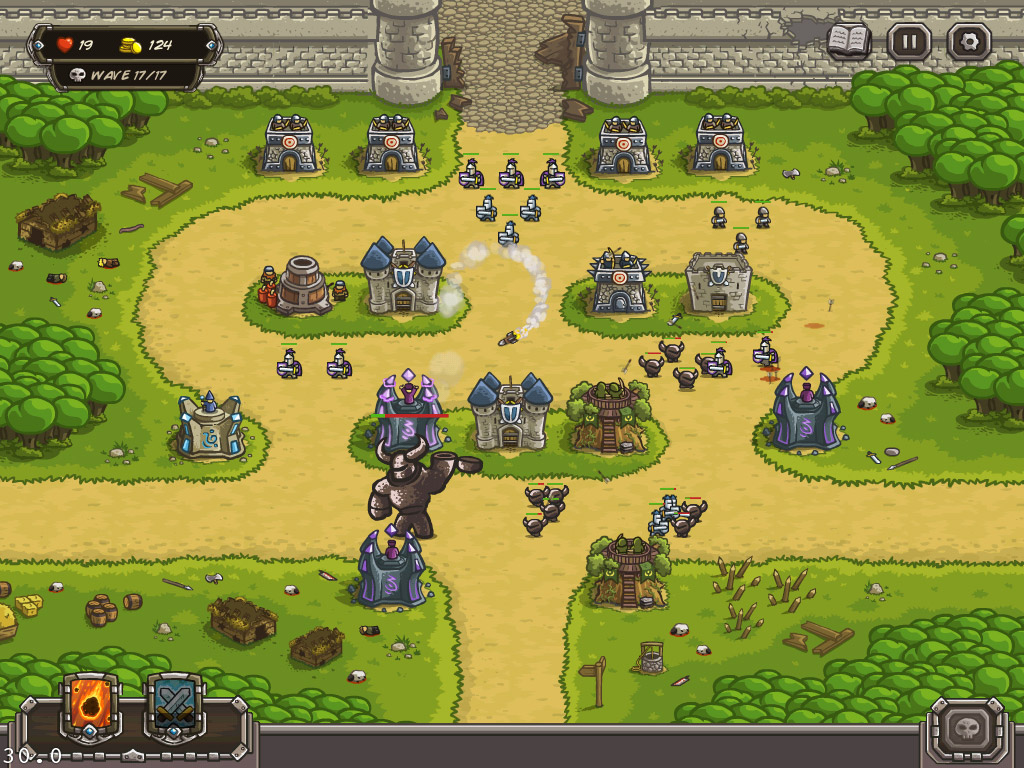
\includegraphics[width=.8\textwidth]{kingdom_rush}
  \caption{Kingdom Rush. Obtida de https://www.ironhidegames.com/Games/kingdom-rush\label{fig:kingdom-rush}}
\end{figure}

\pagebreak

%% ------------------------------------------------------------------------- %%
\section{Shooter}
\label{sec:jogo-ss}

Um \textit{shooter game} é um subgênero de jogos de ação, inspirado pelos jogos de fliperama, por exemplo o jogo  \textit{Spacewar} \citep{Spacewar}, e se estabeleceu com o jogo \textit{Space Invaders} \citep{Space_Invaders}, presente na Figura \ref{fig:space-invaders}. Ambos os jogos funcionam de maneira semelhante, onde uma onda de inimigos deve ser impedida de eliminar o jogador, este podendo se esquivar e atirar neles, sendo que os oponentes também podem dispor de tiros e movimento para causar dano.

%% https://www.gamekult.com/jeux/space-invaders-17318/test.html
\begin{figure}
  \centering
  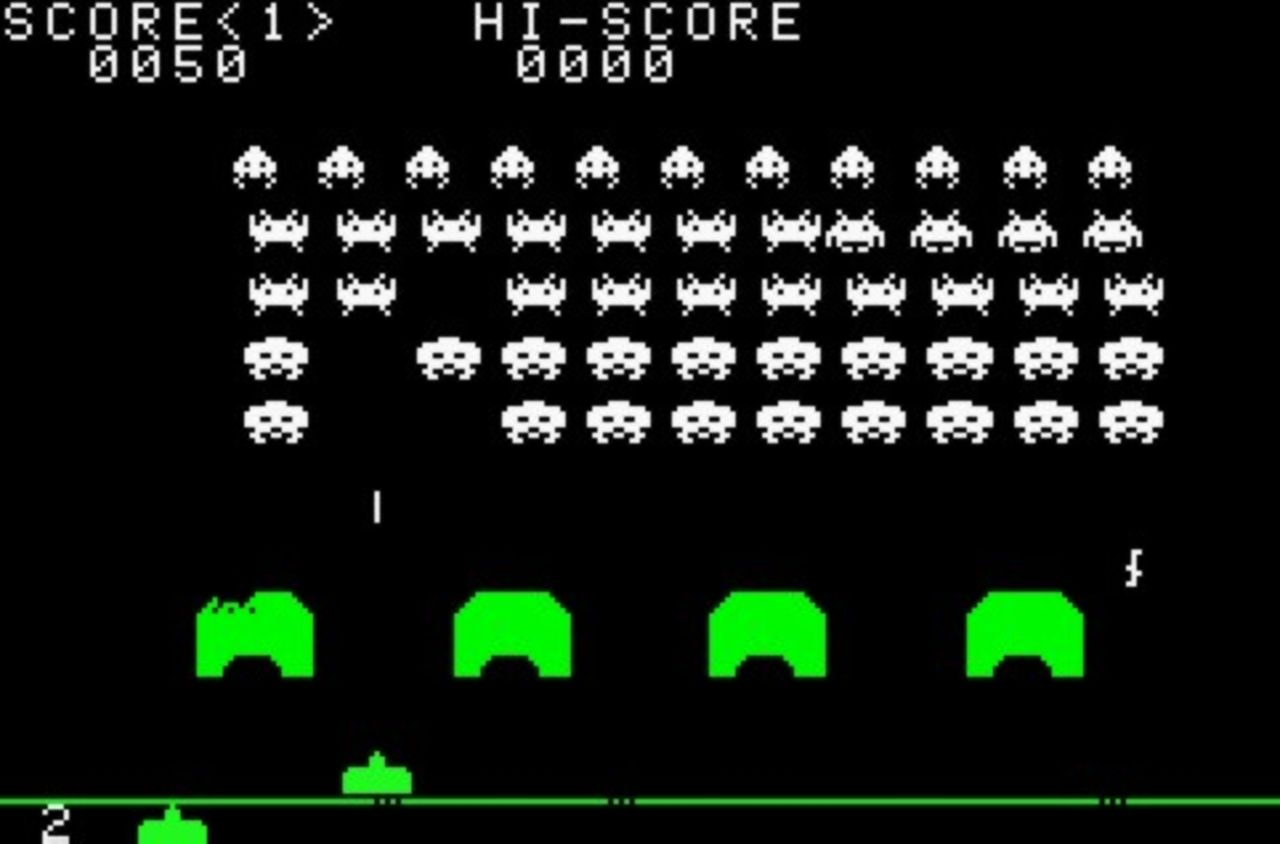
\includegraphics[width=.6\textwidth]{space_invaders}
  \caption{Space Invaders. Obtida de https://www.gamekult.com/jeux/space-invaders-17318/test.html\label{fig:space-invaders}}
\end{figure}

Dentre os elementos comuns ao gênero, existem variações sobre a capacidade do jogador e dos inimigos se moverem no espaço 2D, onde no \textit{Space Invaders} \citep{Space_Invaders}, o jogador possui somente movimento horizontal, enquanto no \textit{Asteroids} \citep{Asteroids}, presente na Figura \ref{fig:asteroids}, o usuário possui movimentação livre em toda área disponível, mas os oponentes não disparam.

%% https://openclipart.org/detail/281726/asteroids-video-games-1979
\begin{figure}
  \centering
  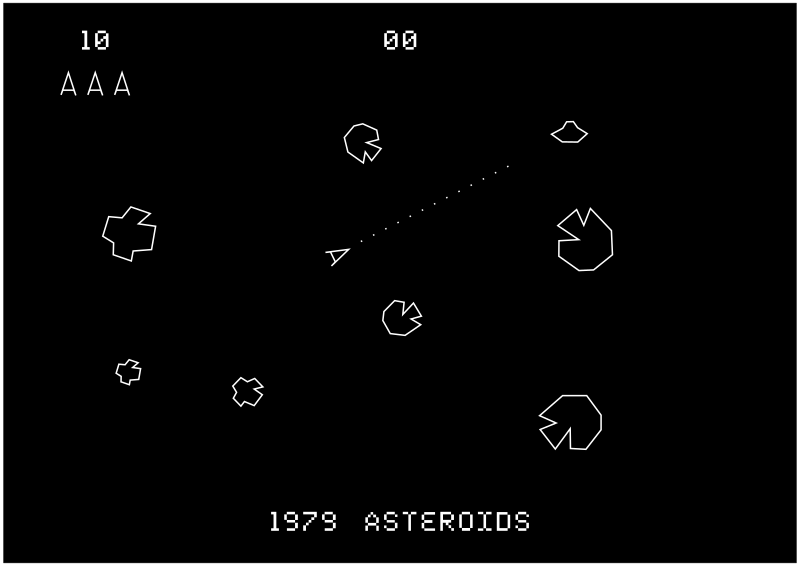
\includegraphics[width=.6\textwidth]{asteroids}
  \caption{Asteroids. Obtida de https://openclipart.org/detail/281726/asteroids-video-games-1979\label{fig:asteroids}}
\end{figure}

%% ------------------------------------------------------------------------- %%
\section{Decisões de Projeto}
\label{sec:jogos-decisoes}

Considerando que são jogos populares e com jogabilidade simples, decidiu-se desenvolver os dois estilos, considerando a simplicidade de seus objetivos em comum, centrados na sobrevivência por meio da habilidade do jogador de se proteger dos inimigos que atacam em turnos, e a possibilidade dos mesmos serem eliminados à distância.

Ao mesmo tempo, enquanto o \textit{Tower Defense} se apresenta de maneira estática - as torres não se movem, e o jogador não pode alterá-las durante a onda - o \textit{Space Shooter} permite movimentação da nave, logo a habilidade motora e reflexos de quem está jogando são fatores na sobrevivência, e seria interessante verificar como essa característica afeta a evolução do algoritmo genético.

Para desenvolver o projeto decidiu-se utilizar ferramentas \textit{Open Source} sempre que possível, a \textit{Godot Game Engine}, versão 3.3.3; a plataforma de versionamento \textit{GitHub}; a comunicação do grupo se concentrou no serviço \textit{Discord}; a monografia foi desenvolvida de maneira colaborativa na plataforma \textit{OverLeaf}; o \textit{Jupyter Notebook} foi utilizado para análise de dados; e o editor de imagens \textit{GIMP} para edição de imagens.
\par

%!TeX root=../tese.tex
%("dica" para o editor de texto: este arquivo é parte de um documento maior)
% para saber mais: https://tex.stackexchange.com/q/78101/183146



%% Nota de rodapé 1: mover para o texto e usar notas de rodapé para citar URLs dos sites de cada engine, com data do último acesso : 

% [p. 7 / § 1] frase de quatro linhas - quebrar em frases mais curtas ou, no caso, montar uma lista de itens. Juntar parágrafo com o seguinte. : X

% [p. 7 / § 2] evitar tantos termos em inglês, principalmente quando eles possuem equivalentes comuns em português:
% open source → código aberto
% license → licença
% game engine → motor de jogos (já que vocês mesmos usaram esse termo no parágrafo anterior)

% Figuras 3.1 e 3.2: citar fonte da imagem : X

% [p. 7 / § 3] escolher ou inglês ou português para se referir aos elementos da Godot e usar de forma consistente (o que ficar em parênteses deve ser só para esclarecer e não o padrão que vocês vão usar). Ajustar no resto da monografia se necessário

% [p. 7 / § 3] sugestão de citação: página de documentação da godot

% [p. 8 / § 2] “todo nó” → “todo nó de colisão/física” ; X
% [p. 8 / § 3] juntar com o parágrafo anterior: X
% [p. 8 / § 3] “programação uma reação” → “programação de uma reação”:X
% [p. 9 / § 4] “figura” -> “Figura” : X

% Figura 3.3: é de vocês? Se for, é legal explicar que ela é do jogo que vocês fizeram. Se não for, citar fonte. : X

% Figura 3.4: se for um exemplo do jogo de vocês, é legal dizer isso. Faltou um ponto final na legenda. : X

% [p. 9 / § 4] typos
% “como um objeto filhos” -> “como objetos filhos” : X

% “a fase geram”: X
% [p. 10 / § 1] juntar com parágrafo anterior : X

%% ------------------------------------------------------------------------- %%
\chapter{Plataforma de Desenvolvimento}
\label{cap:godot}

Para auxiliar na produção de jogos existem diversos motores de jogo ou \textit{Game Engines}; ferramentas que dispõem de recursos e bibliotecas para auxiliar no desenvolvimento. Essas ferramentas oferecem estruturas e métodos para simulação de interações físicas, lidar com a entrada dada pelo usuário, dentre outras funcionalidades. Assim são de grande ajuda para o desenvolvimento do jogo como um todo. A \textit{Godot Engine} é uma  \textit{game engine} de código aberto, usada no desenvolvimento de jogos 2D e 3D, disponibilizada gratuitamente sob \textit{MIT License}. Outros exemplos de \textit{engine} incluem \textit{Unity}\footnote{\url{https://unity.com/pt}}, \textit{Unreal Engine}\footnote{\url{https://www.unrealengine.com/en-US/}} e \textit{RPG Maker}\footnote{\url{https://www.rpgmakerweb.com/}}.


% https://www.unrealengine.com/en-US/
% https://unity.com/pt
% https://www.rpgmakerweb.com/

%% https://godotengine.org/themes/godotengine/assets/press/logo_large_color_light.png
\begin{figure}[htpb]
  \centering
  
\includegraphics[width=.6\textwidth]{godot_logo} 
  \caption{Godot Game Engine.\label{fig:godot-logo} \footnotemark}
\end{figure}
\footnotetext{\url{https://godotengine.org/themes/godotengine/assets/press/logo_large_color_light.png}}

Nesta plataforma, um jogo é um conjunto de cenas composto por nós agrupados em uma estrutura de árvore, estrutura de dado formada por um grafo conexo acíclico. Um nó é a unidade mais básica para construção de elementos, com diferentes propósitos e propriedades, por exemplo, sons, imagens (\textit{sprites}) e câmera. Mesmo com diferentes características e finalidades, todos os nós possuem um nome, variáveis, possibilidade de executarem código (\textit{script}) contendo métodos, herança de funcionalidades ou \textit{script} de outros nós e emissão de sinais de controle para elementos da cena.

\pagebreak

%% https://docs.godotengine.org/en/stable/getting_started/step_by_step/scenes_and_nodes.html
\begin{figure}[htpb]
  \centering
  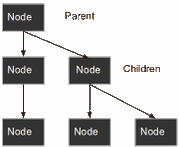
\includegraphics[width=.4\textwidth]{tree}
  \caption{Árvore no Godot.\label{fig:godot-tree} \footnotemark}
\end{figure}
\footnotetext{\url{https://docs.godotengine.org/en/stable/getting_started/step_by_step/scenes_and_nodes.html}}


%% ------------------------------------------------------------------------- %%
\section{Nós}
\label{sec:godot-nos}
 O \textit{Godot} oferece alguns nós específicos para o uso de simulações físicas, fornecendo detecção de colisões entre objetos e diferentes reações caso ocorra o contato. Existem 4 nós específicos para tal função, dependendo do comportamento desejado determinado nó pode ser mais apropriado: \textit{StaticBody2D},  \textit{RigidBody2D}, \textit{KinematicBody2D} e \textit{Area2D}.
 
Todo nó de colisão/física necessita de um filho do tipo \textit{Shape2D} para detectar colisões, pois este fornece a geometria da região que detecta as colisões. Estas podem ocorrer com outros nós ou com as fronteiras da área de jogo. O nó \textit{Area2D} detecta e emite sinais com a presença de outros nós ao seu redor permitindo a programação de uma reação, por exemplo uma esquiva ou animação.

\begin{figure}
  \centering
  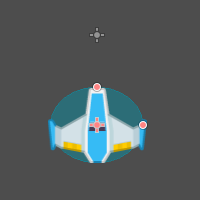
\includegraphics[width=.4\textwidth]{ss/Exemplo area e colisionShape2d.png}
  \caption{Utilizando nós CollisionShape2D e Area2D. Imagem obtida do editor de jogo.\label{fig:area-collision}}
\end{figure}

Na Figura ~\ref{fig:area-collision}, feito para o jogo \textit{Space Shooter}, temos um uso dos nós citados, onde a região em azul sobrepõe a imagem da nave. Esta é um nó do tipo \textit{CollisionShape2D} responsável por detectar colisões com com outros nós, que no jogo são os adversários. A nave por sua vez é um nó do tipo \textit{Area2D} contendo um \textit{sprite} da nave, e quando os nós colidirem, ocorre a emissão de um sinal que terá um comportamento programado, no caso a perda de "vida" do jogador. O conjunto de nós presentes formam uma cena, nesse caso o \textit{Player}.

Nós podem ser agrupados, e o grupo formado atua em conjunto no jogo, conforme a Figura \ref{fig:godot-tree}. O \textit{Tower Defense} e o \textit{SpaceShooter} se aproveitaram de tal característica para a geração dos inimigos e gerenciamento das ondas.

%% ------------------------------------------------------------------------- %%
\section{Sinais}
\label{sec:godot-sinais}

O \textit{Godot} fornece um sistema de sinais, emitidos e detectados por nós, pré-definidos pelo \textit{engine} ou customizados pelo desenvolvedor, que podem servir de gatilhos ou conexões para outras funções em outros nós dentro da hierarquia fornecida pela árvore da cena. As características dos sinais permitem sua utilização em botões na interface, ações em colisões entre nós, entre outras possibilidades.


%% ------------------------------------------------------------------------- %%
\section{Cena}
\label{sec:godot-cena}

A cena no \textit{Godot} é composta de nós organizados segundo uma hierarquia de árvore, onde um nó é a raiz, e seus filhos, que podem ser pais de outros nós, sempre controlados pelo nó raiz, conforme a Figura \ref{fig:scene-tree}, cena feita para o jogo \textit{Space Shooter}. Cenas são objetos independentes, podendo representar somente um elemento do jogo - por exemplo os inimigos, o jogador - ou partes completas dele - como um menu, uma fase.

%% https://docs.godotengine.org/en/stable/getting_started/step_by_step/scenes_and_nodes.html
\begin{figure}
  \centering
  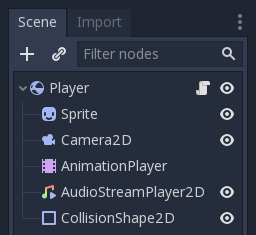
\includegraphics[width=.5\textwidth]{scene_tree_example}
  \caption{Árvore formada por nós no Godot. Em Player um ícone indica a presença de um script vinculado ao nó. Imagem obtida da documentação em \url{https://docs.godotengine.org/en/stable/getting_started/step_by_step/scenes_and_nodes.html}\label{fig:scene-tree}}
\end{figure}



%% ------------------------------------------------------------------------- %%
\section{Instanciação}
\label{sec:godot-instancia}

As cenas de um jogo podem ser inicializadas como objetos filhos de uma outra cena, formando uma instância. Este recurso é usado frequentemente nos jogos desenvolvidos, no \textit{Tower Defense} a fase gera instâncias das cenas das torres e dos inimigos, no \textit{Space Shooter} são instanciados o jogador e os asteróides. As instanciações são feitas de maneira dinâmica durante o jogo, sendo carregadas pelos \textit{scripts} e esperando o \textit{input} do jogador, para a instanciação de um novo objeto que é inserido na árvore de execução. É possível observar o uso da instanciação na Figura \ref{fig:instancia-tiro}, onde a partir do \textit{input} do jogador, projeteis são postos na cena em execução. Cada projetil é uma instanciação, ou objeto, de uma cena feita anteriormente para ser os tiros vistos no jogo.

\begin{figure}
  \centering
  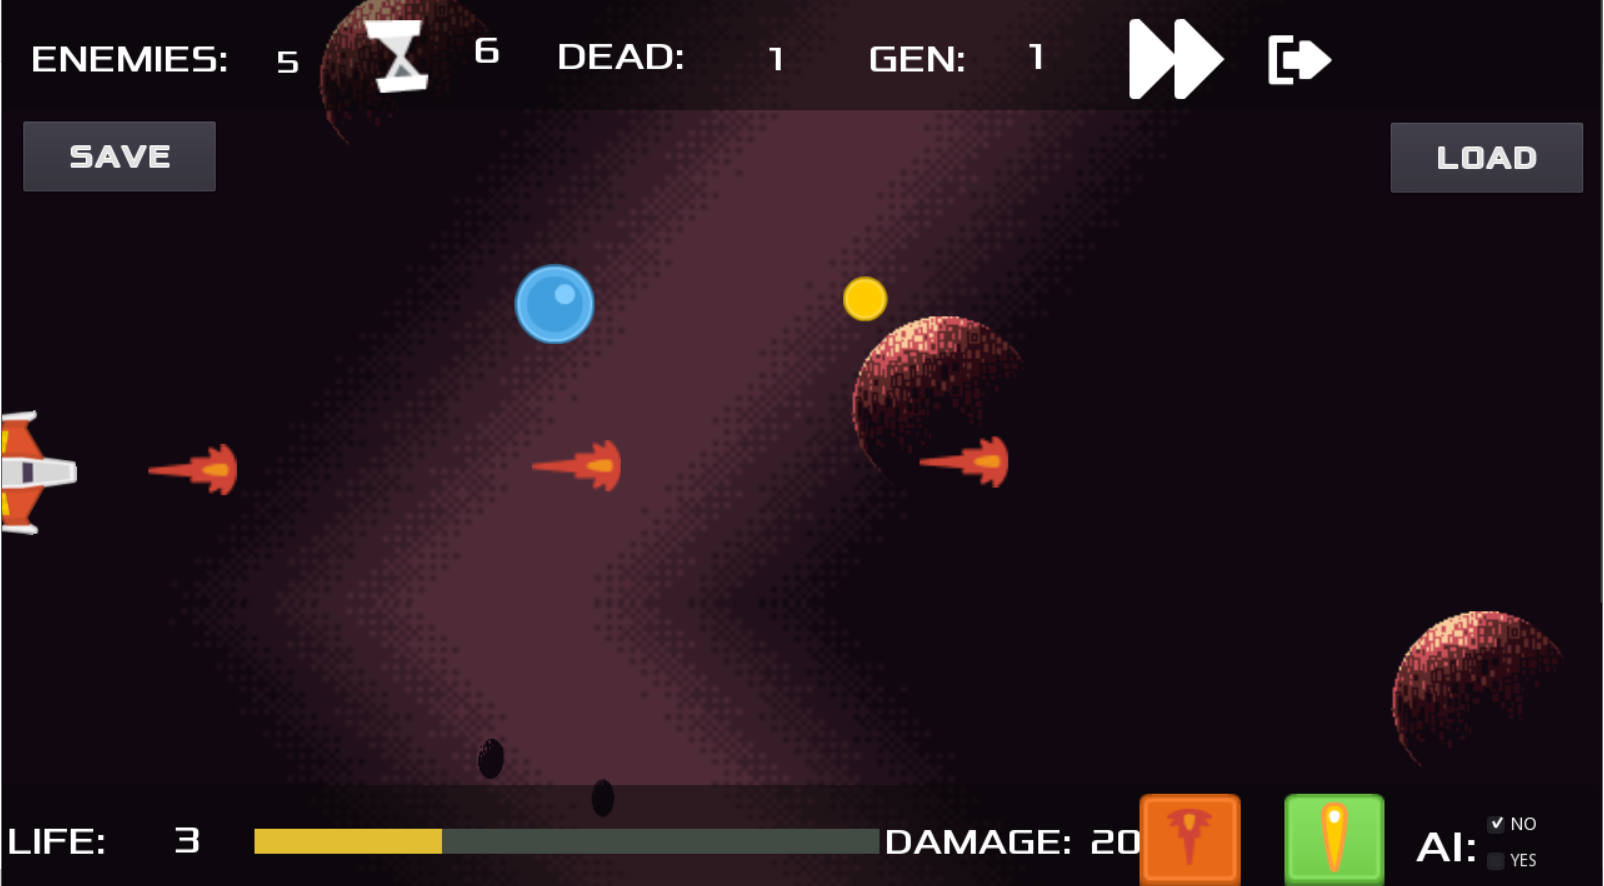
\includegraphics[width=.8\textwidth]{ss/instanciao tiros ss.png}
  \caption{Instanciação de tiros no Space Shooter. Imagem retirada do próprio jogo.\label{fig:instancia-tiro}}
\end{figure}


%% ------------------------------------------------------------------------- %%
\section{Singletons}
\label{sec:godot-singleton}

\textit{Singletons} fornecem a possibilidade de acesso global a métodos e variáveis de outras classes no \textit{Godot}. Semelhante aos sinais, os \textit{singletons} oferecem comunicação entre cenas distintas, relevantes no projeto pois permitiu a implementação do algoritmo genético, que necessita de acesso a diversas variáveis dos jogos, como os inimigos, dano causado, entre outros.

%% ------------------------------------------------------------------------- %%
\section{GDscript}
\label{sec:godot-gdscript}

% Recomendação Will: juntar paragrafos.

Os \textit{scripts} citados são escritos em \textit{GDscript}, linguagem de programação dinâmica de alto nível desenvolvida especificamente para a \textit{Godot Engine}, similar a linguagem de programação \textit{Python} e \textit{Lua}, porém com otimizações e tipos de dados específicos, altamente integrado à própria \textit{engine}\citep{godot-faq}. O editor fornecido integra diversas funcionalidades de um ambiente de desenvolvimento avançado em sua interface, como editor visual 2D e 3D, editor de texto, conexões de sinais, depurador, visualização da árvore de execução durante o desenvolvimento e em tempo real durante a execução, que facilitam o início da produção de jogos.

%% ------------------------------------------------------------------------- %%
\section{Desenvolvimento dos jogos}
\label{sec:desenvolvimento}


% Mencionar o uso de licenças abertas
Para facilitar a familiarização com o ambiente de desenvolvimento e acelerar o foco no algoritmo genético, foram utilizados diversos recursos disponíveis para a produção dos jogos. Desde repositórios de \textit{sprites} como \citet{Kenny_sprites} a tutoriais de \textit{Godot}, sendo o \textit{Space Shooter} baseado no tutorial de \citet{Godot_Linietsy}, disponível na documentação da \textit{engine}, enquanto o \textit{Tower Defense} foi baseado no tutorial disponibilizado pelo \citet{GameDevelopmentCenter21:tdtutorial}. Tanto \citet{Kenny_sprites} como \citet{Godot_Linietsy} possuem licenças que permitem o uso publico ou equivalente, além de serem gratuitas.  

\par

%!TeX root=../tese.tex
%("dica" para o editor de texto: este arquivo é parte de um documento maior)
% para saber mais: https://tex.stackexchange.com/q/78101/183146

%% ------------------------------------------------------------------------- %%

%Recomendação WILL: 
% Ao invés de mecânica colocar design : X
% TD Mencionar Tabelas : X
% TD Mencionar Figuras 4.1 , 4.2, 4.4, 4.5 : X
% SS Mencionar Tabelas : 4.3,  4.4: X
% SS Mencionar Figuras:  4.7, 4.8, 4.9, 4.10, 4.11, 4.12:X

\chapter{Design dos jogos}
\label{cap:mecanica-dos-jogos}

O desenvolvimento dos jogos foi focado em características comuns entre si, para possibilitar o uso do mesmo algoritmo genético, minimizando a necessidade de ajustes no código. A implementação inicial foi feita no \textit{Tower Defense}, e em seguida no \textit{Space Shooter}.

%% ------------------------------------------------------------------------- %%
\section{Tower Defense}
\label{sec:mj-td}

\subsection{O jogo}
\label{sub-sec:jogo-td}

O jogo \textit{Tower Defense} \footnote{Repositório contendo o jogo: { \url{https://github.com/raktanaka/tccTD} - 21/12/2021}} consiste em mapa com dois caminhos a serem percorridos por tanques inimigos e oferece ao jogador duas torres para impedir que os tanques completem seu trajeto. O início do percurso é na esquerda da tela, terminando na direita, conforme visto na Figura \ref{fig:td-inicial}.

\begin{figure}
  \centering
  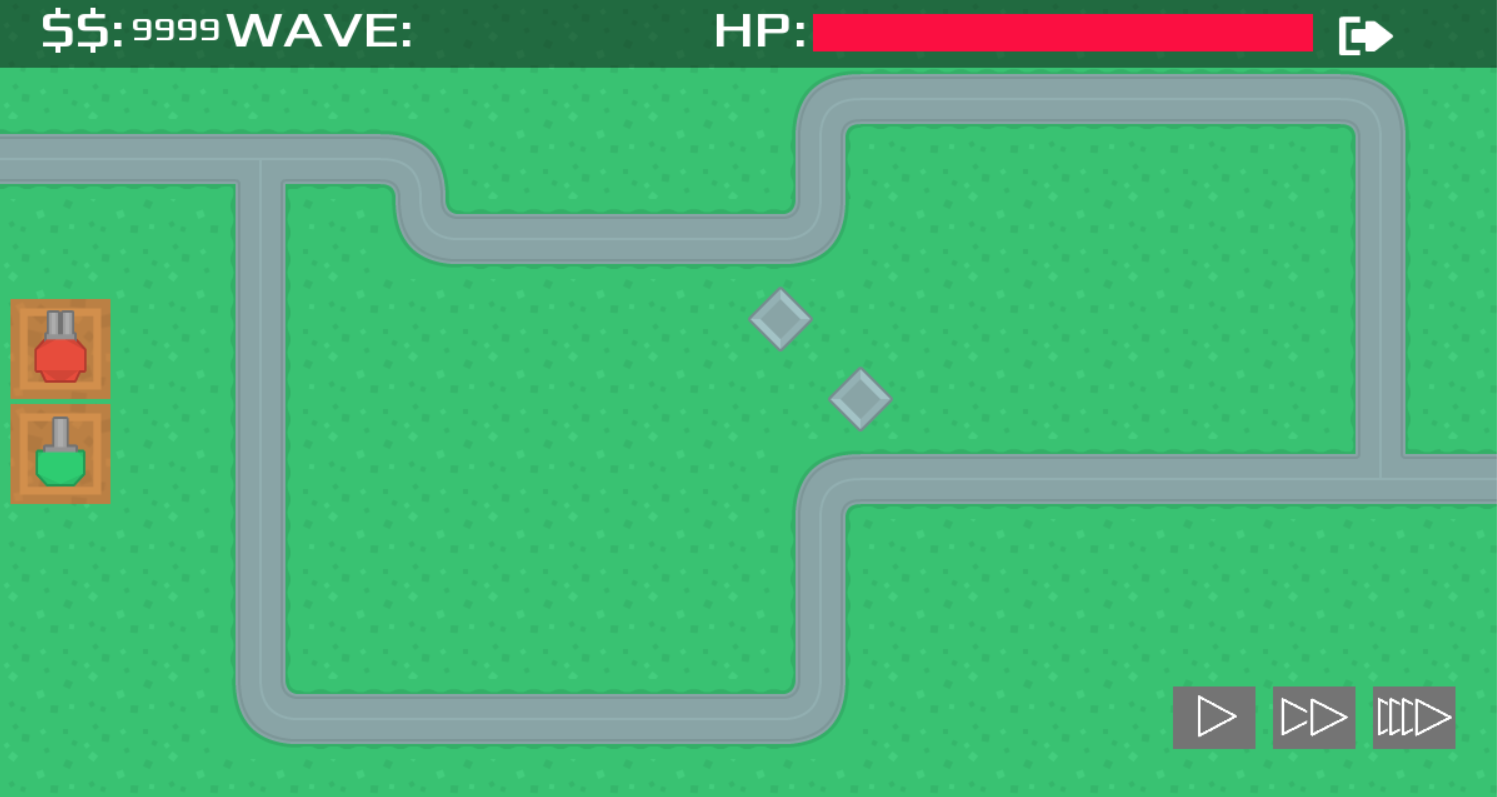
\includegraphics[width=\textwidth]{td/Mapa_inicial_tDD.png}
  \caption{Tela Inicial. Imagem retirada do próprio jogo.\label{fig:td-inicial}}
\end{figure}

Antes de apertar o botão \textit{Play}, o jogador pode colocar quantas e quaisquer torres desejar em áreas livres do mapa. Iniciando a partida, uma onda de 12 tanques começa a percorrer o caminho, inicialmente 6 para cada percurso, conforme a Figura \ref{fig:td-exemplo}. Posteriormente, o algoritmo genético gerencia a rota. Ao lado do botão \textit{Play} estão botões que aceleram a execução do jogo em duas vezes e oito vezes, para facilitar a coleta de dados para os testes.

As duas torres disponíveis oferecem diferentes áreas de alcance para detecção de tanques, apresentadas nas Figuras \ref{fig:td-range-gree} e \ref{fig:td-range-red} e quantidade de dano que podem causar, como esta descrito na Tabela \ref{tab:dados_torres}. Cada inimigo que atinge o objetivo produz dano ao jogador, que possui 100 pontos de vida, mostrado pela barra \textit{HP} na tela. A região também mostra os recursos monetários disponíveis ao jogador - que não está implementado - e a onda atual; o jogo somente termina quando acaba o \textit{HP} do jogador.

\begin{figure}
  \centering
  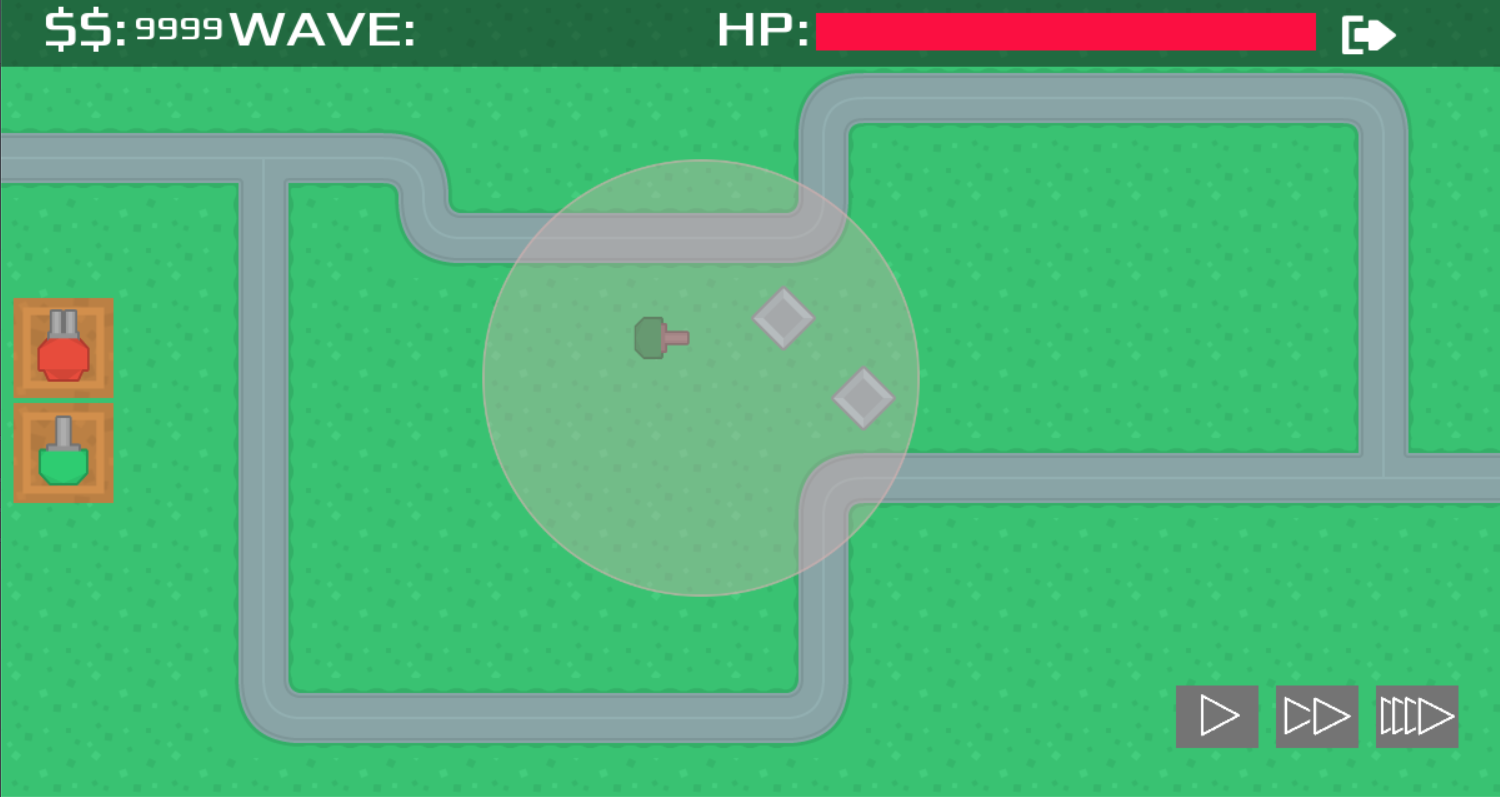
\includegraphics[width=0.8\textwidth]{td/range_green_tower.png}
  \caption{Área de detecção torre verde. Imagem retirada do próprio jogo.\label{fig:td-range-gree}}
\end{figure}

\begin{figure}
  \centering
  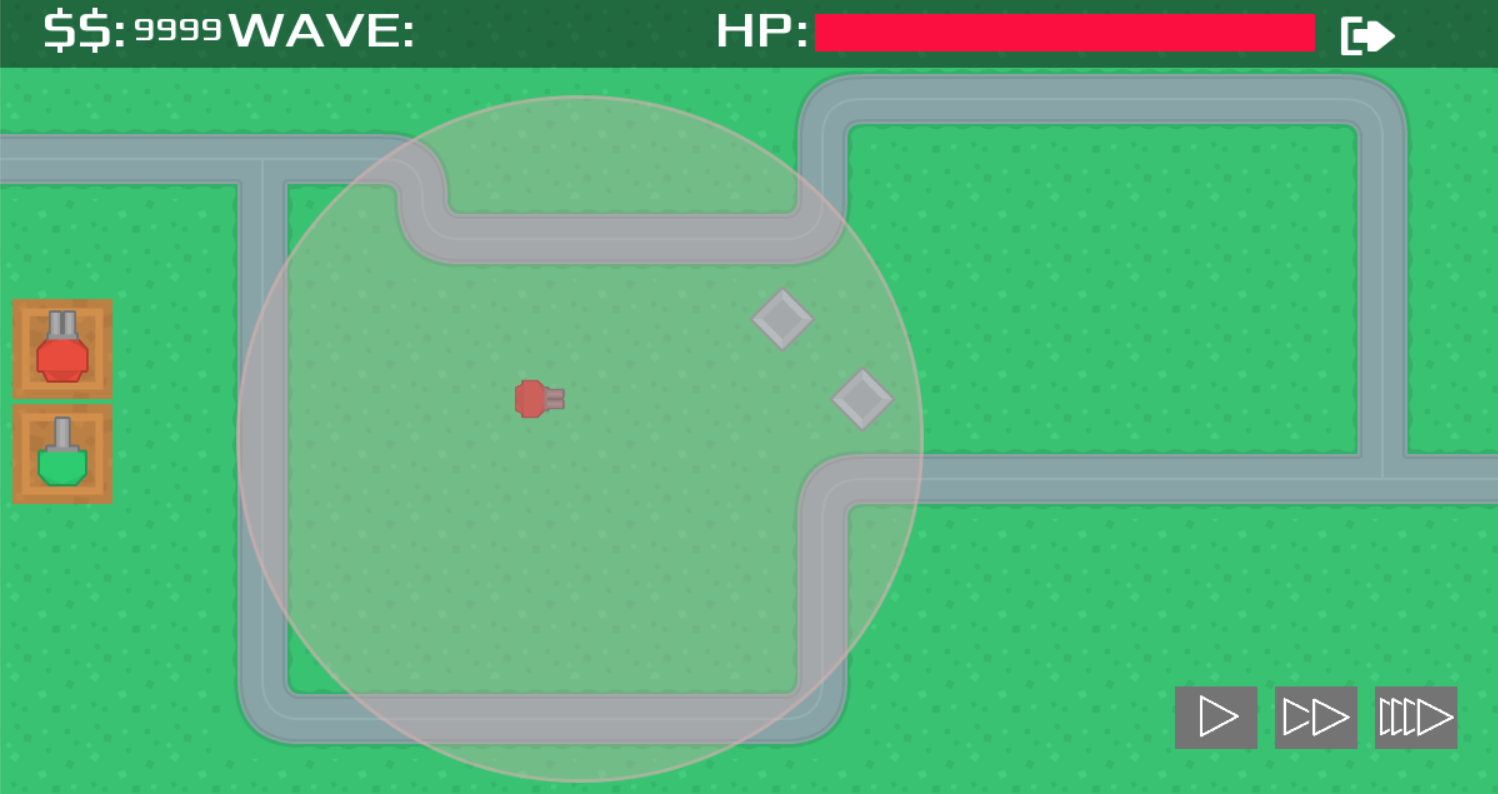
\includegraphics[width=0.8\textwidth]{td/range_red_tower.png}
  \caption{Área de detecção torre vermelha. Imagem retirada do próprio jogo.\label{fig:td-range-red}}
\end{figure}

\begin{table}[H]
\caption{Dano das torres no Tower Defense.\label{tab:dados_torres}}
\begin{tabular}{c|ccc}

               & velocidade de tiro  & dano   & alcance\\ \hline
Torre Verde    & 55                  & 25     &  350 \\
Torre Vermelha & 70                  & 15     &  550       

\end{tabular}
\end{table}


\begin{figure}
  \centering
  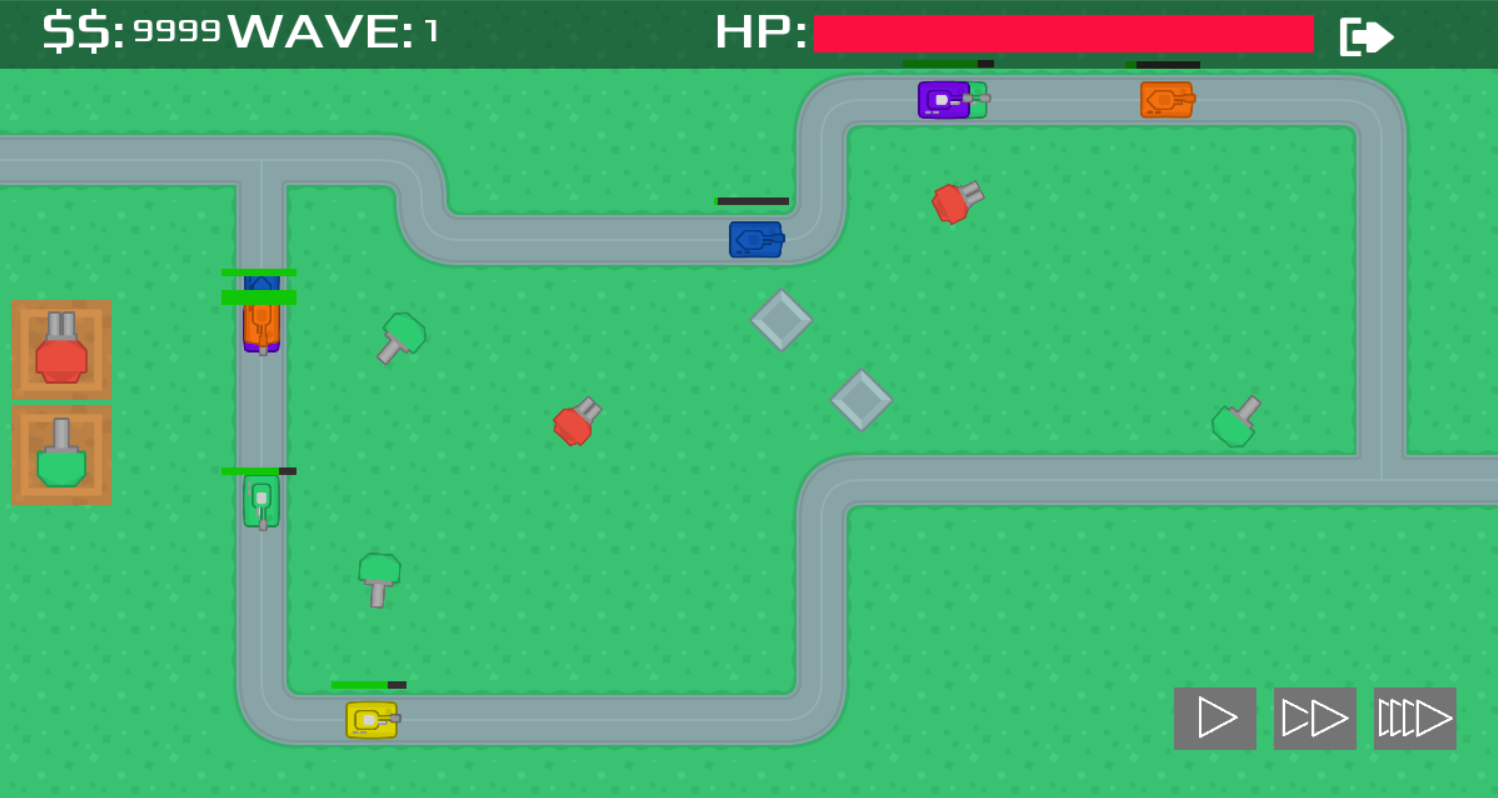
\includegraphics[width=\textwidth]{td/exemplo de execução TDD.png}
  \caption{Exemplo de uma execução do jogo. Imagem retirada do próprio jogo.\label{fig:td-exemplo}}
\end{figure}


Existem 6 tipos de tanques diferentes, descritos na Figura \ref{fig:figure-tipos-tanque}. Cada tipo de tanque possui 2 características, sendo elas velocidade e dano causado ao jogador, cujo os valores variam conforme o tipo, visto a Tabela \ref{tab:tank-dmg}. 

\begin{figure}
     \centering
     \begin{subfigure}[b]{0.2\textwidth}
         \centering
         
\includegraphics[width=\textwidth]{td/tank_blue.png}
         \caption{tank blue}
         \label{fig:td-tank-blue}
     \end{subfigure}
     \hfill
     \begin{subfigure}[b]{0.2\textwidth}
         \centering
         
\includegraphics[width=\textwidth]{td/tank_green.png}
         \caption{tank green}
         \label{fig:td-tank-green}
     \end{subfigure}
     \hfill
     \begin{subfigure}[b]{0.2\textwidth}
         \centering
         
\includegraphics[width=\textwidth]{td/tank_red.png}
         \caption{tank red}
         \label{fig:td-tank-red}
     \end{subfigure}
     
     \begin{subfigure}[b]{0.2\textwidth}
         \centering
         
\includegraphics[width=\textwidth]{td/tank_orange.png}
         \caption{tank orange}
         \label{fig:td-tank-orange}
     \end{subfigure}
     \hfill
     \begin{subfigure}[b]{0.2\textwidth}
         \centering
         
\includegraphics[width=\textwidth]{td/tank_purple.png}
         \caption{tank purple}
         \label{fig:td-tank-purple}
     \end{subfigure}
     \hfill
     \begin{subfigure}[b]{0.2\textwidth}
         \centering
         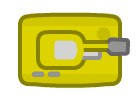
\includegraphics[width=\textwidth]{td/tank_yellow.png}
         \caption{tank yellow}
         \label{fig:td-tank-yellow}
     \end{subfigure}     
     \caption{Tipos de tanques}
     \label{fig:figure-tipos-tanque}
\end{figure}

\newpage

\begin{table}
\caption{Dano de cada tanque no Tower Defense}
\begin{tabular}{c|cc}
            & velocidade & dano   \\ \hline
tank blue   & 55    & 55         \\
tank green  & 70    & 45         \\
tank red    & 80    & 15          \\
tank orange & 120   & 5           \\
tank purple & 90    & 15          \\
tank yellow & 150   & 5           
\end{tabular}
\label{tab:tank-dmg}
\end{table}

Ficam definidas como Norte e Sul as rotas disponíveis, na Figura \ref{fig:td-rota}.

\begin{figure}
  \centering
  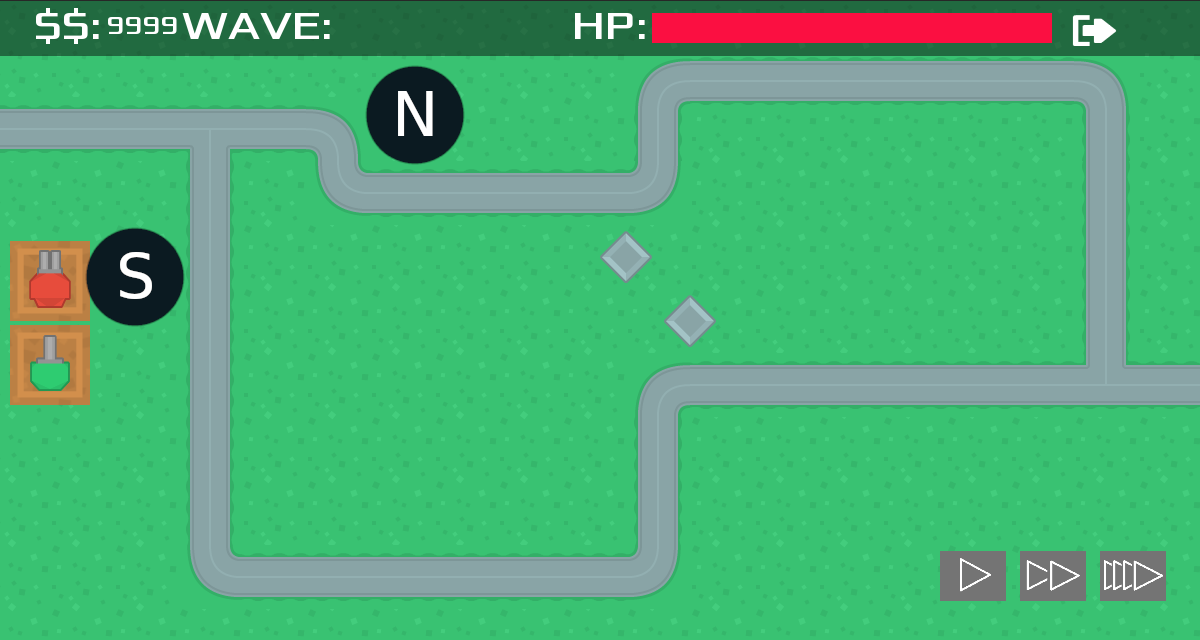
\includegraphics[width=\textwidth]{td/td_positions.png}
  \caption{Definição das rotas Norte e Sul. Imagem retirada do jogo e editada.\label{fig:td-rota}}
\end{figure}

\subsection{Mecânica de Resistência}
\label{sub-sec:mecanica-de-resistencia}

No jogo de \textit{Tower Defense} também foi adicionado um sistema de resistência nos tanques, cada Tanque possui resistência contra Torres de \textbf{mesma cor} e recebem dano reduzido pela metade dos mesmos. Segue um pseudocódigo da implementação do tanque ao receber dano de uma torre.

\begin{programruledcaption}{Sistema de Resistência TD.\label{prog:resistencia-TD}}
  \begin{lstlisting}[
    language={[brazilian]pseudocode},
    style=pseudocode,
    style=wider,
    functions={},
    specialidentifiers={},
  ]
        // x = tanque que recebe o dano
        // damage = quantidade total de dano recebido
        // color\_tower = cor da torre que disparou no tanque.
        func on_hit(x, damage, color_tower):
            // color (x) = cor do tanque \textbf{x}
            //  hp(x) = hp atual de x.
	        se color (x) = color_tower:
		        hp (x) -= damage / 2
		
        	senao:
        		hp (x) -= damage
        fim
  \end{lstlisting}
\end{programruledcaption}


\newpage
%% ------------------------------------------------------------------------- %%
\section{Space Shooter}
\label{sec:mj-ss}

O jogo \textit{Space Shooter}\footnote{Repositório contendo o jogo { \url{https://github.com/RGPRafael/godot} - 21/12/2021}} consiste em uma nave que o jogador pode mover livremente em um espaço 2D, onde este deve sobreviver a ondas de asteroides que partem de diferentes posições da tela em sua direção. O jogador além de esquivar, pode eliminar os asteroides por meio de disparos com o \textit{mouse}. 

\begin{figure}
  \centering
  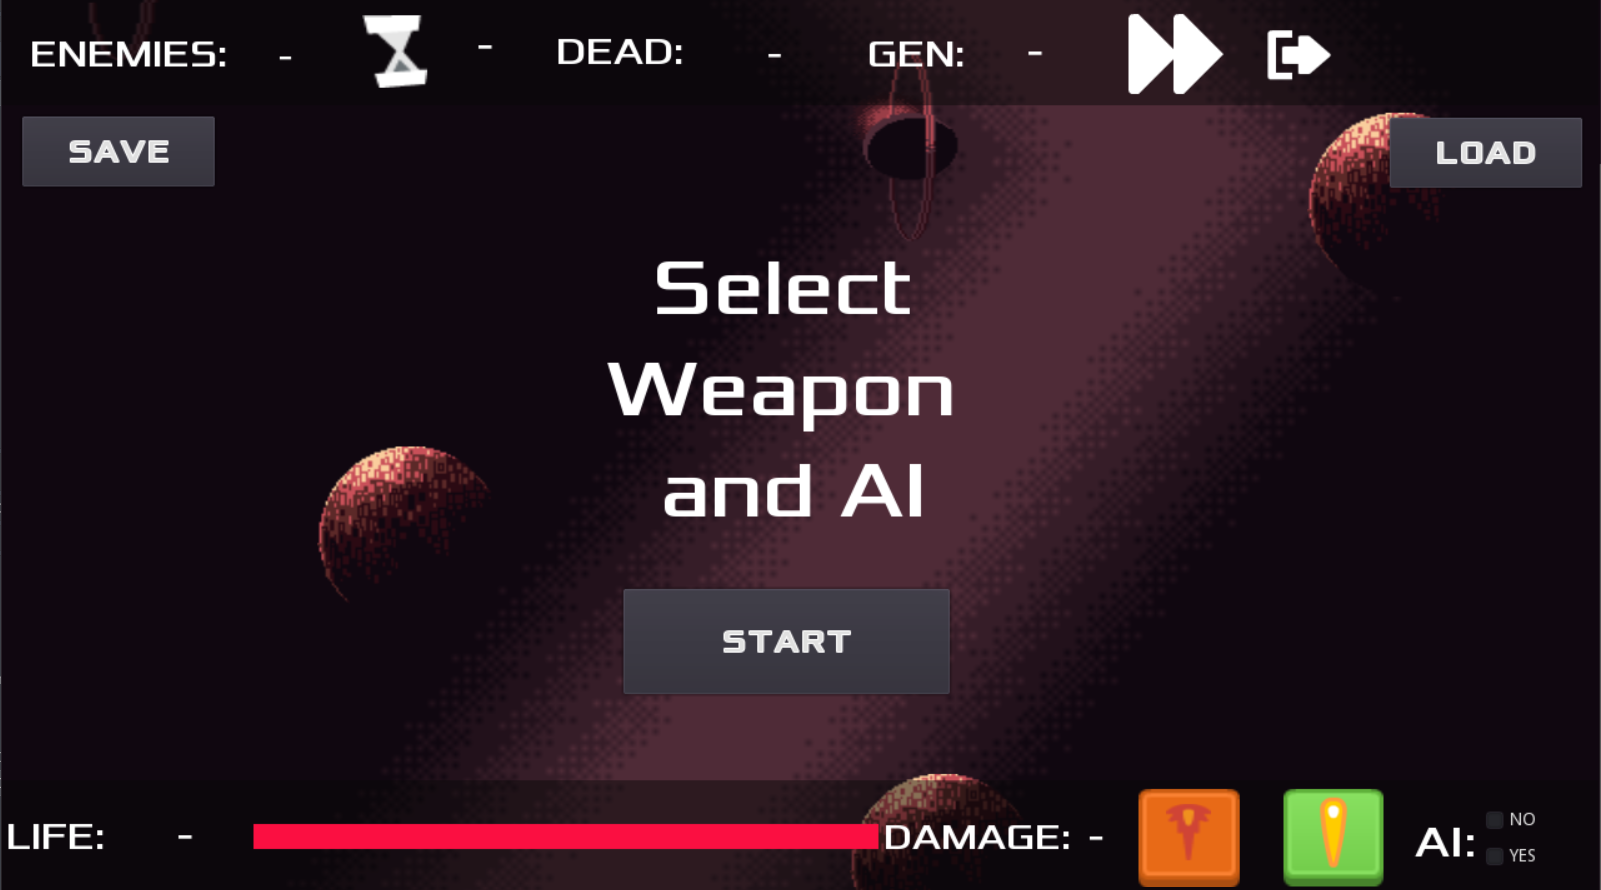
\includegraphics[width=\textwidth]{ss/Tela_inicial_space_shooter.png}
  \caption{Tela inicial. Imagem retirada do próprio jogo.\label{fig:ss-start}}
\end{figure}

Existem dois tipos de disparos que o jogador pode usar para sua defesa, cada um com características diferentes. No começo do jogo é requisitado que o jogador escolha qual tipo de disparo irá utilizar, conforme as Figuras \ref{fig:ss-start} e \ref{fig:ss-disparos}.

\begin{figure}
     \centering
     \begin{subfigure}[b]{0.15\textwidth}
         \centering
         
\includegraphics[width=\textwidth]{ss/Disparo_.png}
         \caption{Disparo}
         \label{fig:ss-disparo}
     \end{subfigure}
     \begin{subfigure}[b]{0.15\textwidth}
         \centering
         
\includegraphics[width=\textwidth]{ss/Disparo1_.png}
         \caption{Disparo1}
         \label{fig:ss-disparo1}
     \end{subfigure}
     \caption{Disparos}
     \label{fig:ss-disparos}
\end{figure}

\begin{table}
\caption{Dano dos tiros no Space Shooter}
\begin{tabular}{c|cc}
          & Velocidade de Tiro & Dano \\ \hline
Disparo   & 1200  & 15     \\
Disparo 1 & 600   & 30    
\end{tabular}
\label{tab:tiro=-ss}
\end{table}

Existem dois tipos de \textit{player} automáticos disponíveis para escolha, caso o jogador marque a opção \textit{'yes'} na barra inferior, próximo ao texto \textit{'AI'}, como pode se observar na Figura \ref{fig:ss-player-ai}. Tais \textit{players} foram desenvolvidos com o intuito de auxiliar no projeto, e na realização dos testes e coleta de dados. Uma delas faz com que a nave transite da direita para esquerda em um intervalo de cinco minutos, a outra opção faz com que a nave fique parada no meio da tela, em ambos atirando no inimigo mais próximo que detectar, de forma a destruir o asteroide que vem em sua direção ou ser atingida.  

\begin{figure}
  \centering
  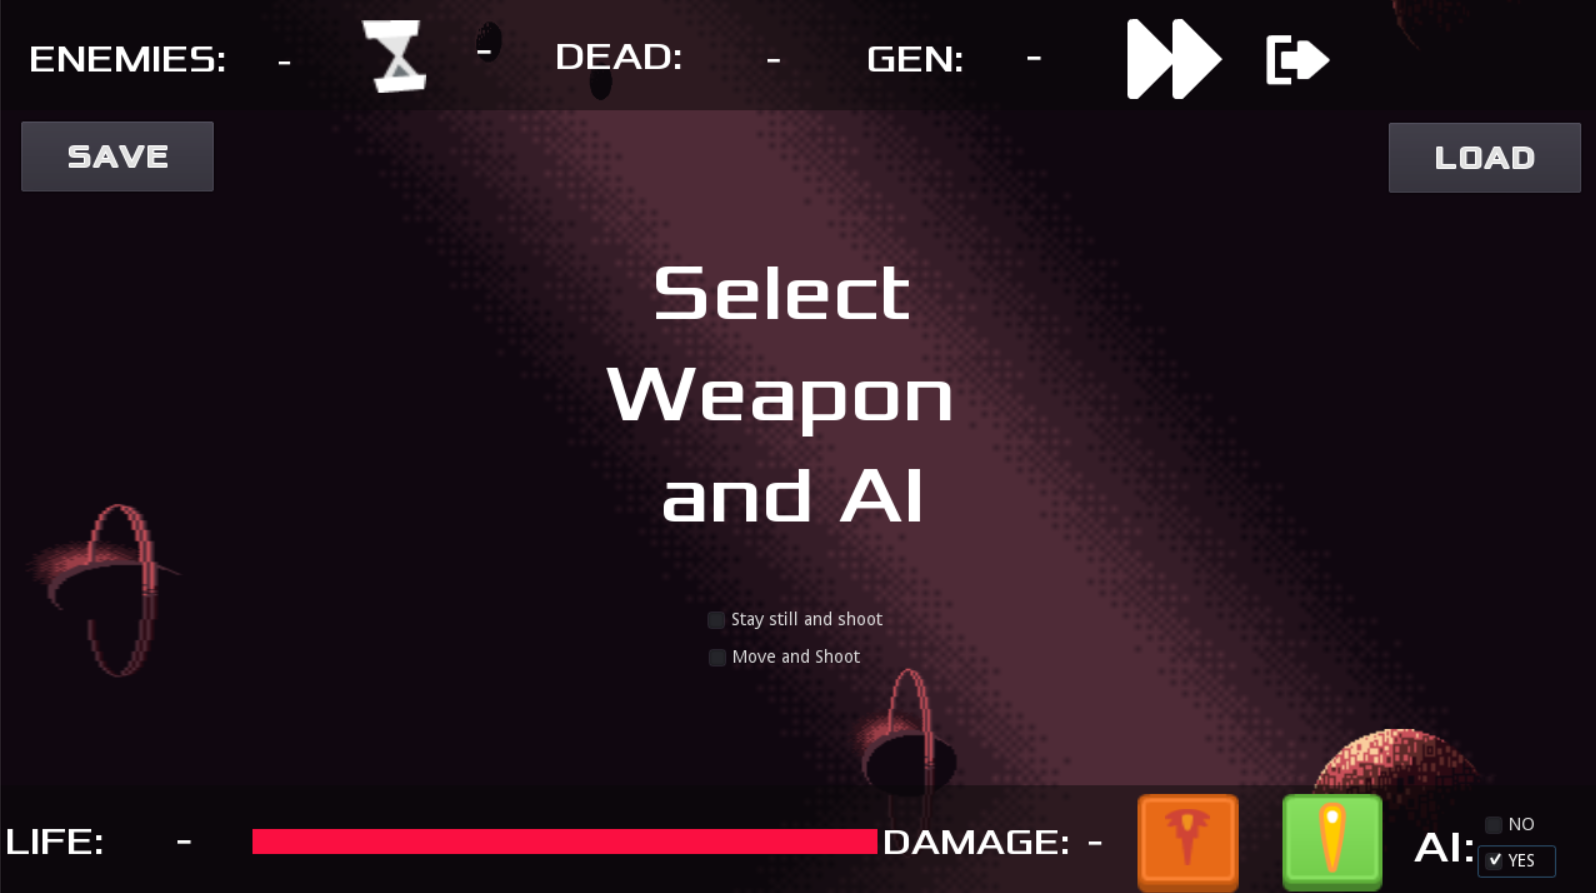
\includegraphics[width=\textwidth]{ss/Escolhendo player automatico.png}
  \caption{Opções de Player Automático. Imagem retirada do próprio jogo.\label{fig:ss-player-ai}}
\end{figure}


Existem 6 tipos de asteroides diferentes, presentes na Figura \ref{fig:ss-tipo-ast}. Cada tipo de asteroide possui 3 características, sendo elas velocidade, vida ou resistência e dano causado ao jogador, cujo os valores variam conforme o tipo, presentes na Tabela \ref{tab:ss-ast-dmg}. 

\begin{figure}
     \centering
     \begin{subfigure}[b]{0.15\textwidth}
         \centering
         
\includegraphics[width=\textwidth]{ss/inimigos.png}
         \caption{inimigos}
         \label{fig:ss-inimigos}
     \end{subfigure}
     \hfill
     \begin{subfigure}[b]{0.15\textwidth}
         \centering
         
\includegraphics[width=\textwidth]{ss/inimigo1.png}
         \caption{inimigo1}
         \label{fig:ss-inimigo1}
     \end{subfigure}
     \hfill
     \begin{subfigure}[b]{0.15\textwidth}
         \centering
         
\includegraphics[width=\textwidth]{ss/inimigo2.png}
         \caption{inimigo2}
         \label{fig:ss-inimigo2}
     \end{subfigure}

     \begin{subfigure}[b]{0.15\textwidth}
         \centering
         
\includegraphics[width=\textwidth]{ss/inimigo3.png}
         \caption{inimigo3}
         \label{fig:ss-inimigo3}
     \end{subfigure}
     \hfill
     \begin{subfigure}[b]{0.15\textwidth}
         \centering
         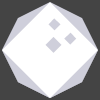
\includegraphics[width=\textwidth]{ss/inimigo4.png}
         \caption{inimigo4}
         \label{fig:ss-inimigo4}
     \end{subfigure}
     \hfill
     \begin{subfigure}[b]{0.15\textwidth}
         \centering
         
\includegraphics[width=\textwidth]{ss/inimigo5.png}
         \caption{inimigo5}
         \label{fig:figure-inimigos}
     \end{subfigure}     
     \caption{Tipos de asteroides}
     \label{fig:ss-tipo-ast}
\end{figure}

\begin{table}[H]
\caption{Velocidade, dano e vida de cada asteroide no Space Shooter}
\begin{tabular}{c|ccc}
         & Velocidade & Dano & Vida   \\ \hline
inimigos & 500        & 20     &   50     \\
inimigo1 & 350        & 45     &   30     \\
inimigo2 & 470        & 50     &   40     \\
inimigo3 & 320        & 60     &   40     \\
inimigo4 & 550        & 20     &   60     \\
inimigo5 & 700        & 10     &   120      
\end{tabular}
\label{tab:ss-ast-dmg}
\end{table}

Após feitas as escolhas sobre o tipo de disparo que será utilizado e se o jogador vai mover a nave ou não, basta apertar o botão \textit{'Start'} para inicio do jogo. O jogador assim deve sobreviver às ondas de inimigos que aparecem de diferentes posições da tela. 

Caso seja atingido, a quantidade de dano que sofreu é exibida no campo \textit{'Damage'}. Por sua vez, quantidade de inimigos que apareceram enquanto o jogo ainda se desenrola é mostrada na barra superior na extrema esquerda, assim como outras informações como numero de asteroides que foram mortos e o números de gerações que foram enfrentadas. Há um botão para acelerar a velocidade do jogo, e outro que volta ao começo do jogo, caso o jogador não queria continuar ou tenha se arrependido das configurações iniciais que fez anteriormente, um exemplo de uma rodada do jogo encontra-se na Figura \ref{fig:ss-exemplo}.

\begin{figure}
  \centering
  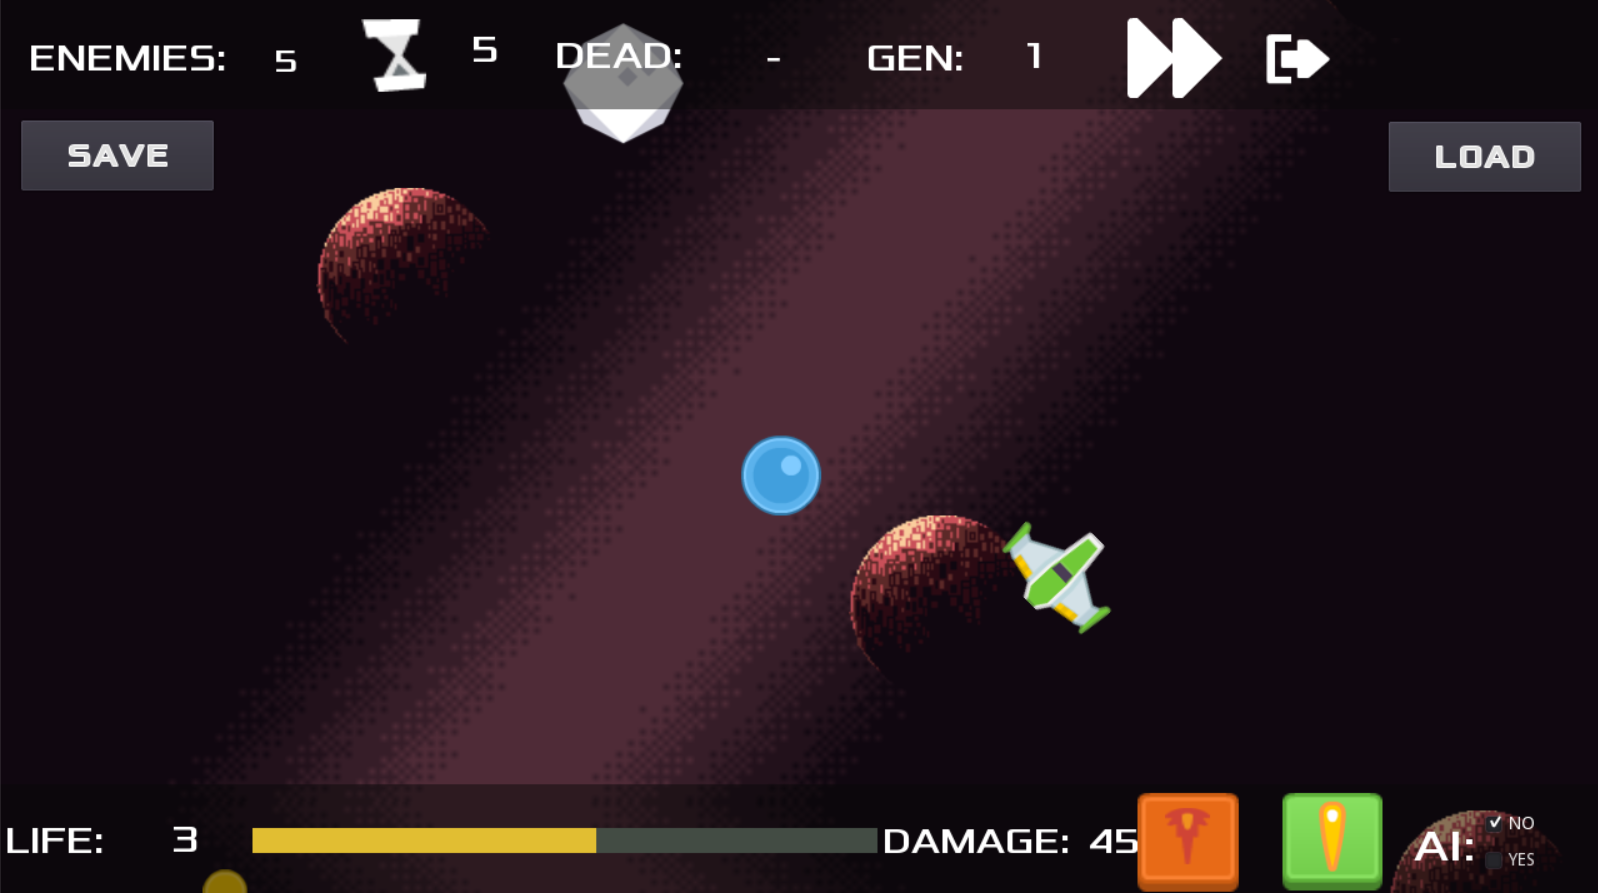
\includegraphics[width=\textwidth]{ss/Exemplo de jogo.png}
  \caption{Exemplo de uma rodada do jogo. Imagem retirada do próprio jogo.\label{fig:ss-exemplo}}
\end{figure}

O jogador começa com a sua barra de vida no valor total igual a 100. Caso chegue a zero 3 vezes o jogador morre e o jogo volta à tela inicial onde as configurações sobre a escolha de arma, por exemplo, devem ser feitas de novo. Ficam definidos os locais de \textit{spawn} de 1 até 6 na Figura \ref{fig:ss-positions}

\begin{figure}
  \centering
  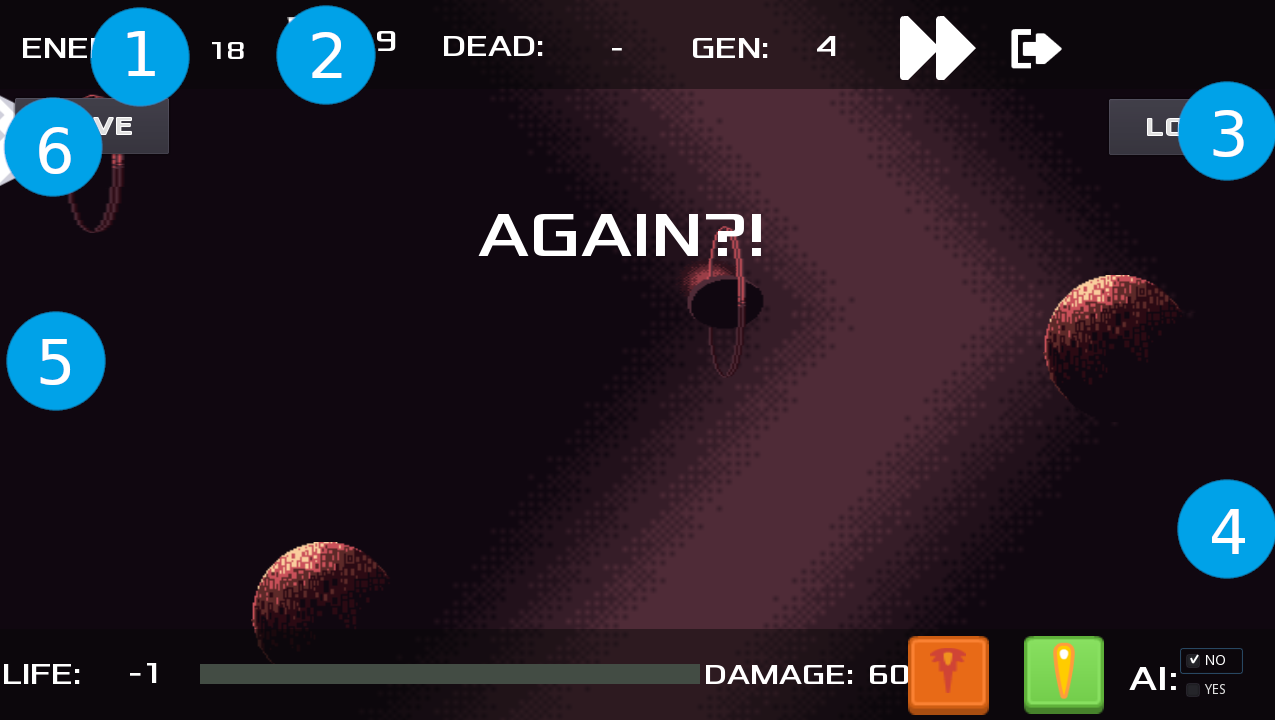
\includegraphics[width=\textwidth]{ss/ss_positions.png}
  \caption{Posições possíveis onde um asteroide pode surgir. Imagem retirada do jogo e editada.\label{fig:ss-positions}}
\end{figure}
\par

%!TeX root=../tese.tex
%("dica" para o editor de texto: este arquivo é parte de um documento maior)
% para saber mais: https://tex.stackexchange.com/q/78101/183146

%% ------------------------------------------------------------------------- %%
\chapter{Algoritmo Genético}
\label{cap:algoritmo-genetico}

Algoritmo genético é uma técnica de evolução computacional desenvolvida para o estudo de comportamento adaptativo \citep{eiben15:introga}. De maneira simplificada, o algoritmo cria um conjunto de diferentes resoluções para um dado problema e, a partir da avaliação desse conjunto, seleciona as melhores soluções.

Esse processo imita a ideia de seleção natural proposta por Darwin \citep{eiben15:introga}, onde os indivíduos de uma população disputam por recursos para sobreviverem. Aqueles que sobrevivem conseguem passar seus genes para a prole e a população seguinte será mais adaptada ao ambiente e com mais chances de reprodução, passando as características que permitiram sua sobrevivência para as gerações seguintes. Portanto, um algoritmo genético é composto das seguintes etapas: Inicialização, Avaliação, Seleção, Cruzamento \textit{(Cross over)}, Mutação e Atualização (Figura ~\ref{fig:alg-genetico} ).

%% ------------------------------------------------------------------------- %%
\section{O Algoritmo}
\label{sec:ag-algoritmo}

No projeto, cada indivíduo é um inimigo criado pelo jogo e a população se resume a uma \textit{"wave"} (onda de inimigos). Os genes representam características importantes dos inimigos, como: Tipo (TD e SS), Rota (TD), Local de \textit{Spawn} (SS), conforme esboçado por \citet{mallawaarachchi:gatutorial} e \citet{ahmed18:tutorialgapython}.

%% FALTA REFERÊNCIA DA IMAGEM
\begin{figure}
  \centering
  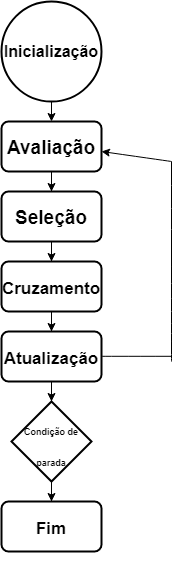
\includegraphics[width=4cm]{alg_genetico2}
  \caption{Estrutura de um algoritmo genético.\label{fig:alg-genetico}}
\end{figure}


%% ------------------------------------------------------------------------- %%
\subsection{Inicialização}
\label{sec:ag-inicializacao}

Na primeira etapa, inicialização, são codificados os genes para que sejam submetidos ao processo de avaliação. 

\pagebreak

\begin{programruledcaption}{Inicialização do \textit{Space Shooter} com tipo de inimigo e local de surgimento.\label{prog:init-ss}}
  \begin{lstlisting}[
    language={[brazilian]pseudocode},
    style=pseudocode,
    style=wider,
    functions={},
    specialidentifiers={},
  ]
var population = [['inimigos',Vector2(90,-50) ], 
                 ['inimigo1',Vector2(90,-50)], 
                 ['inimigo2',Vector2(90,-50)], 
                 ['inimigo3',Vector2(90,-50)], 
                 ['inimigo4',Vector2(90,-50) ],
                 ['inimigo5',Vector2(90,-50)]]
  \end{lstlisting}
\end{programruledcaption}

\begin{programruledcaption}{Inicialização do \textit{Tower Defense} com tipo de inimigo e rota.\label{prog:init-td}}
  \begin{lstlisting}[
    language={[brazilian]pseudocode},
    style=pseudocode,
    style=wider,
    functions={},
    specialidentifiers={},
  ]
var population = [['EnemyRed', 0], ['EnemyGreen', 0], ['EnemyBlue', 0],
                 ['EnemyYellow', 0], ['EnemyPurple', 0], ['EnemyOrange', 0],
                 ['EnemyRed', 1], ['EnemyGreen', 1], ['EnemyBlue', 1],
                 ['EnemyYellow', 1], ['EnemyPurple', 1], ['EnemyOrange', 1]]
  \end{lstlisting}
\end{programruledcaption}

No \textit{Tower Defense} o algoritmo inicia com uma população de 12 inimigos, 1 de cada tipo para cada rota; no \textit{Space Shootes} são 1 de cada tipo em cada posição de \textit{spawn}. Uma amostra que pareceu adequada para o propósito do experimento, uma vez que populações pequenas convergem mais rapidamente, economizando tempo para múltiplas execuções,e não tem indícios de serem piores do que largas populações. \citet{haupt00:mutationprob}

%% ------------------------------------------------------------------------- %%
\subsection{Avaliação}
\label{sec:ag-avaliacao}

A avaliação (ou função \textit{Fitness}) realiza uma análise que estabelece o quão bem os indivíduos da população resolvem o problema proposto. Na natureza, se trata da habilidade de um indivíduo competir contra os demais da população, no algoritmo proposto segue:

\begin{programruledcaption}{\textit{Fitness} do \textit{Tower Defense} (Avaliação, em português).\label{prog:avaliacao_TD}}
  \begin{lstlisting}[
    language={[brazilian]pseudocode},
    style=pseudocode,
    style=wider,
    functions={},
    specialidentifiers={},
  ]
        funcao fitness_TD (x) // Dá uma pontuação para indivíduo \textbf{x}
            // offset (x) = quanto do caminho foi percorrido, float de 0 a 1.
            // hp (x)     = quanto de HP sobrou do inimigo, float de 0 a 1.
	        fit := (offset (x) + hp (x)) / 2 // média aritmética dos valores de x
	        devolva fit // Um float com uma pontuação no intervalo [0,1].
        fim
  \end{lstlisting}
\end{programruledcaption}

\begin{programruledcaption}{\textit{Fitness} do \textit{Space Shooter} (Avaliação, em português).\label{prog:avaliacao_SS}}
  \begin{lstlisting}[
    language={[brazilian]pseudocode},
    style=pseudocode,
    style=wider,
    functions={},
    specialidentifiers={},
  ]
        funcao fitness_SS (x) // Dá uma pontuação para indivíduo \textbf{x}
            // reached-goal (x) = booleana se acertou o inimigo ou nao
            se reached-goal
                fit := 5
            senao
                fit := 0
            
            // hp(x) = 5 * quanto de HP sobrou do inimigo (mob), no intervalo [0,1]
	        fit := (fit + hp(x)) / 10 // média aritmética dos valores de x
	        devolva fit // Um float com uma pontuação no intervalo [0,1].
        fim
  \end{lstlisting}
\end{programruledcaption}

Deve ser ressaltado que o \textit{fitness} é uma característica inerente a cada sistema, com múltiplas possibilidades de avaliação que produzem resultados que podem ser considerados corretos, encontrando máximos locais que satisfazem os problemas propostos.

%%
%% FALTA REFERÊNCIA DA IMAGEM
%%\begin{figure}
%%  \centering
%%  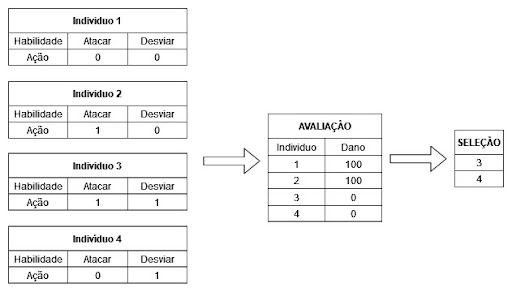
\includegraphics[width=.8\textwidth]{tabel_gen_2}
%%  \caption{Exemplo de seleção para o algoritmo genético.\label{fig:figure}}
%%\end{figure}

%% ------------------------------------------------------------------------- %%
\subsection{Seleção}
\label{sec:ag-selecao}

Na etapa de seleção, os indivíduos são selecionados para reprodução com base na sua aptidão obtida anteriormente. O algoritmo seleciona 2/3 dos indivíduos como a melhor abordagem, em ordem decrescente dos valores de \textit{fitness}, com base na natureza (2 pais geram 1 filho). Contudo, os experimentos e consulta a referências, mostraram que a escolha do tamanho da prole não é trivial. \citep{jansen05:offspring}

%% ------------------------------------------------------------------------- %%
\subsection{Cruzamento}
\label{sec:ag-cruzamento}

No cruzamento, as soluções são recombinadas gerando novos indivíduos, tomando parte dos genes do pai e da mãe (dois indivíduos distintos na população); sendo considerada metade dos genes do pai e da mãe, gerando 1/3 dos indivíduos para a próxima geração. A Figura \ref{fig:crossover} a seguir ilustra o cruzamento, onde \textit{crossover point} representa o ponto em que os genes foram divididos, com os retângulos vermelhos representando características que a IA selecionou de cada um dos pais.

\begin{figure}
  \centering
  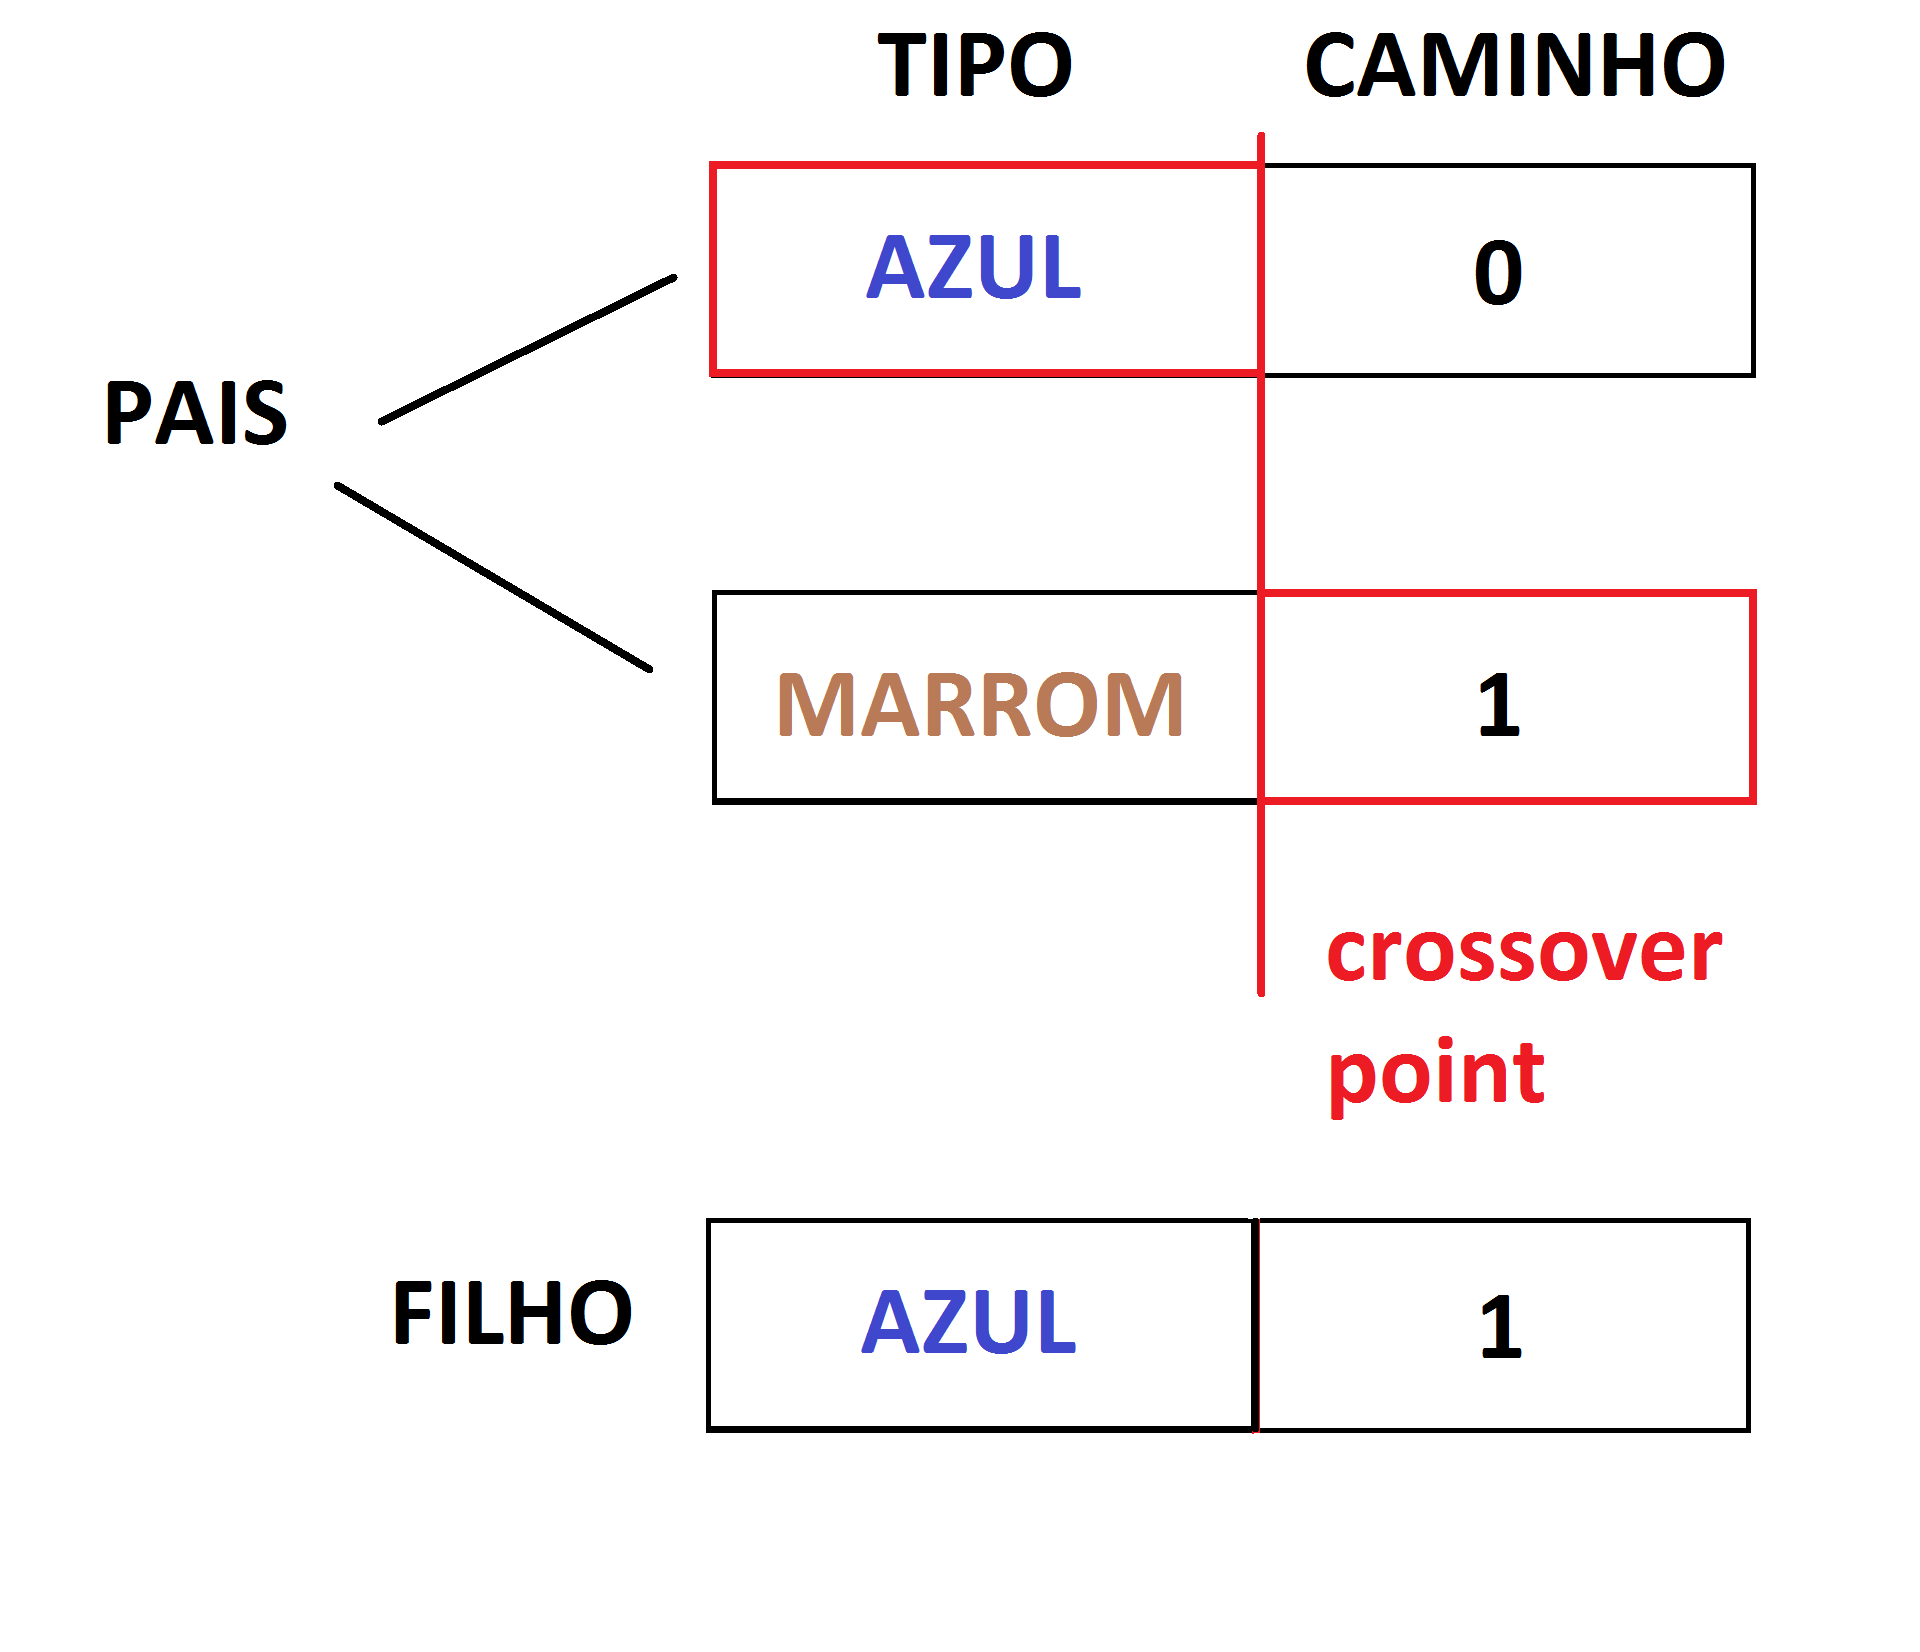
\includegraphics[width=.4\textwidth]{crossover}
  \caption{\textit{Crossover} para o caso do TD.\label{fig:crossover}}
\end{figure}

%% ------------------------------------------------------------------------- %%
\subsection{Mutação}
\label{sec:ag-mutacao}

A mutação representa a parte do algoritmo que equilibra '\textit{exploitation vs exploration}', ou seja, o quanto o algoritmo deve continuar buscando novas soluções (\textit{exploration}) ou o quanto ele deve continuar tirando vantagem da solução que já encontrou (\textit{exploitation}). No caso do algoritmo genético implementado, a mutação pode ocorrer em um único gene de um ou mais indivíduos da população, adicionando variabilidade ao resultado final. \citep{eiben98:exploitvsexplore}. 

No caso do trabalho, como os testes tinham rigor mais determinístico (pela implementação), era esperado que a população final convergisse para algum resultado. Portanto, a taxa de mutação escolhida foi de $\frac{1}{\text{nº de individuos na pop}} = \frac{1}{12} ou \frac{1}{6}$. Uma taxa que pareceu adequada conforme o artigo de \citet{haupt00:mutationprob}.

\pagebreak

%% ------------------------------------------------------------------------- %%
\subsection{Atualização}
\label{sec:ag-atualizacao}

Os indivíduos resultantes serão adicionados na população na etapa de atualização  e, caso seja necessário, o processo descrito acontece novamente.

\begin{programruledcaption}{Resumo do código. \label{prog:resumo_AG}}
  \begin{lstlisting}[
    language={[brazilian]pseudocode},
    style=pseudocode,
    style=wider,
    functions={},
    specialidentifiers={},
  ]
    funcao start_experiment (pop) // Cria uma nova população baseada na população atual
        // Quantidade de pais para reprodução
        num_parents_mating := population.size() * 2 / 3
	
	    // Função de Avaliação dos pais mais aptos da população
	    fitness := cal_pop_fitness(population_res)
	
	    // Função de Seleção dos melhores candidatos para a reprodução
	    parents := select_mating_pool(population, fitness, num_parents_mating)
	
	    // offspring\_size [0] = quantidade de filhotes
	    // offspring\_size [1] = quantidade de genes
	    // length(pop) = quantidade de individuos em pop
	    // genes(pop) = quantidade de genes de qualquer individuo de pop
	    offspring_size := [length(pop) - parents.size(), genes(pop)]
	    
	    // Função de Cruzamento dos pais para gerar os filhos.
	    offspring_crossover := crossover (parents, offspring_size)

	    // Função de Mutação dos filhos
	    offspring_mutation := mutation (offspring_crossover)
	    
	    // Adiciona os pais que sobreviveram de volta no vetor população
	    para i = 0 até tamanho (parents):
		    new_population.append (parents[i])
		fim
		    
		// Adiciona a nova prole para a população
	    para i = 0 até tamanho (offspring_mutation):
		    new_population.append (offspring_mutation[i])
		fim

	    devolva new_population
    fim
  \end{lstlisting}
\end{programruledcaption}
\par

%!TeX root=../tese.tex
%("dica" para o editor de texto: este arquivo é parte de um documento maior)
% para saber mais: https://tex.stackexchange.com/q/78101/183146

%% ------------------------------------------------------------------------- %%


% Recomendação Will: mudar nome do cap para método de avaliação do algoritmo ou similar: X

% ao invés de usar delineamento usar design ou desenho: X

% colocar uma tabela ou imagem ilustrando o uso do quadrado latino no nosso trabalho: 

% colocar nota de rodapé em desenvolvimento primeiro paragrafo referente a ultimo acesso e URL site:X

% WILL : "Qual a diferença de atributos entre os diferentes tanques e torres mesmo? Acho que vocês mencionam antes no texto mas é bom repetir, mover para aqui, ou pelo menos referenciar a seção onde foi dito": X

% Mencionar figuras no texto: X

% Mencionar Tabelas no texto: X

% deixar mais claro que soluções ingenuas servem para ser comparadas com algoritmo genético.: X

% Figuras sempre com letra maiúscula quando for mencionar no texto:X



\chapter{Método de Avaliação do algoritmo}
\label{cap:testes}

Com o algoritmo funcional, foi necessário buscar maneiras de avaliar seu desempenho para garantir sua eficiência \textit{versus} inimigos gerados aleatoriamente. Foram consideradas as possibilidades de distribuir os jogos e coletar \textit{feedback} de outros jogadores, mas considerando possíveis avaliações subjetivas para os jogos relativamente simples e limitações de tempo decidiu-se por utilizar métodos automatizados para coleta de resultados de dano em sequências de ondas.

%% ------------------------------------------------------------------------- %%
\section{Metodologia}
\label{sec:t-metodologia}

Segundo o Teorema Central do Limite, são necessárias, no mínimo, 30 amostras para que a média das mesmas tenha uma distribuição aproximadamente normal \citep{Magalhaes_estatistica}. Portanto, foram planejados experimentos nos jogos para geração de 30 amostras de dados em cada modo de jogo, para produção de gráficos com o comportamento das ondas, e desenho em quadrado latino.

%% ------------------------------------------------------------------------- %%
\subsection{Quadrado Latino}
\label{sec:t-quad-latino}

A coleta e disposição dos dados teve como objetivo a montagem de um quadrado latino.
Um quadrado latino de v linhas por v colunas é um arranjo de v letras latinas na forma de uma tabela, de maneira que cada letra ocorra apenas uma vez em cada linha, e uma vez em uma coluna, \citep{Design_exp_latin_sq}. Por exemplo, a tabela 3 x 3 é um quadrado latino:

\begin{table}
\caption{Exemplo de quadrado latino}
\begin{tabular}{ccc}
    A       & B    & C     \\ 
    B       & C    & A     \\
    C       & A    & B      \\
\end{tabular}
\end{table}

O desenho em quadrado latino é usado em experimentos onde os objetos de estudo estão submetidos a uma series de tratamentos, onde o tempo decorrido terá influência significativa nas respostas \citep{Design_exp_latin_sq}. A escolha do desenho em quadrado latino também é apropriada dado que os ambientes em que os testes foram feitos não são exatamente iguais, e por existirem dois fatores que podem influenciar nas respostas\citep{campbell:quadradolatino} - a inteligência artifical e o jogador que está sendo simulado.


%% ------------------------------------------------------------------------- %%
\section{Experimentos com o Algoritmo}
\label{sec:t-testes-algoritmo}

Durante o decorrer dos experimentos, notou-se incoerências nos testes realizados pelos códigos produzidos. Em especial, na função \textit{fitness} e na taxa de mutação.

\subsection{Fitness}

A função de avaliação (\textit{fitness}) é passada pelo usuário do código e, portanto, tiveram que ser criadas. No próximo capítulo \ref{sec:a-fitness}, será explicado mais detalhadamente sobre os resultados produzidos com diferentes funções de avaliação (\textit{fitness}) e as tentativas de alcançar outros resultados com base nelas.

\subsection{Taxa de mutação}

A taxa de mutação também pode ser definida pelo  usuário. Em particular, para testes pequenos como os feitos neste trabalho, é recomendado um valor entre $5\%$ até $20\%$. \citep{haupt00:mutationprob}.

Uma diferente abordagem ainda nesse tópico, é a utilização de taxas de mutação que decrescem conforme o tempo. Possui seus benefícios em testes de natureza mais determinística, já que espera-se que o algoritmo chegue em um ponto de convergência nas populações finais. Este método proporciona maior \textit{exploration} nas gerações iniciais, uma vez que está buscando o melhor resultado sem se prender em pontos de máximo local e maior \textit{exploitation} nas gerações finais, pois estará explorando o melhor resultado que obteve até o momento. \citep{eiben98:exploitvsexplore}

%% ------------------------------------------------------------------------- %%
\section{Desenvolvimento}
\label{sec:t-desenvolvimento}

Para fazer a coleta dos dados de maneira mais eficiente, os jogos foram adaptados para armazenarem os resultados das ondas. Foram desenvolvidas cenas no \textit{Godot} (menus e fases de teste), como pode se ver nas Figuras \ref{fig:tela-de-teste-tower defense} e \ref{fig:tela-de-teste-space-shooter}, que executam os testes de maneira determinística e consistente, sem aceitar \textit{input} do jogador. O botão \textit{Test Mode} acessa a interface de testes, enquanto o botão \textit{Play Defaut mode} utiliza o modo de jogo padrão. Todos os resultados são gravados em arquivos ".txt" com nome e formatação pré-definidos para facilitar a análise exploratória dos dados em \textit{Jupyter Notebook} \footnote{ \url{https://github.com/raktanaka/tcc-results} - 21/12/2021}.

\pagebreak

\begin{figure}
  \centering
  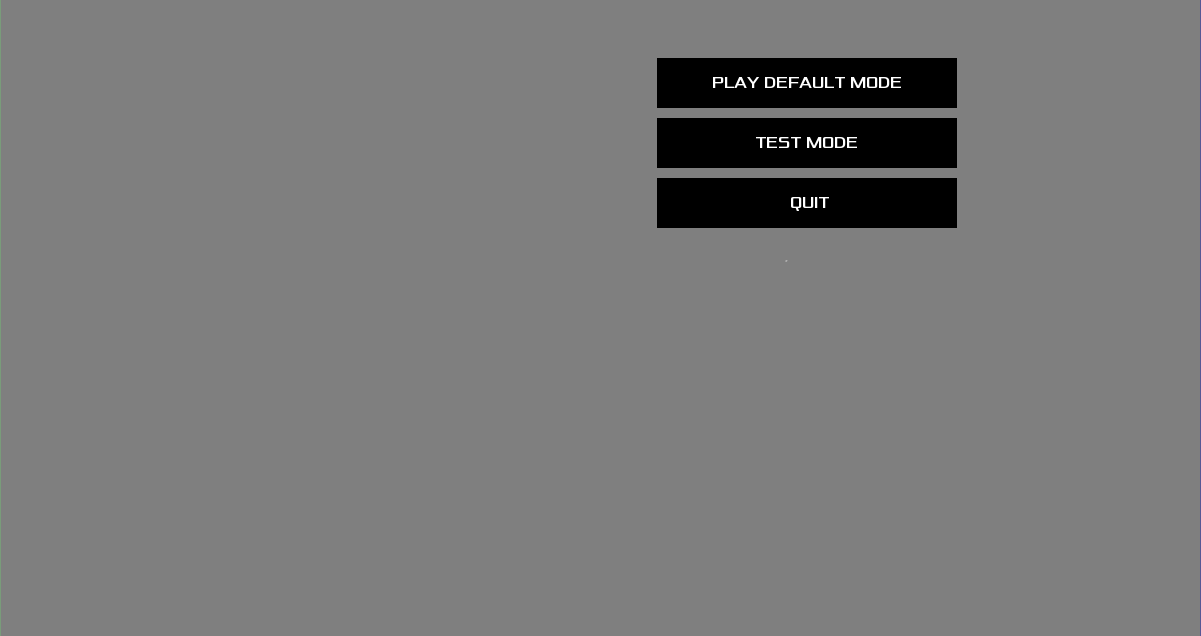
\includegraphics[width=.8\textwidth]{td/Tela_Teste_TDD.png}
  \caption{Tela de Teste Tower defense. Imagem retirada do próprio jogo.\label{fig:tela-de-teste-tower defense}}
\end{figure}

\begin{figure}
  \centering
  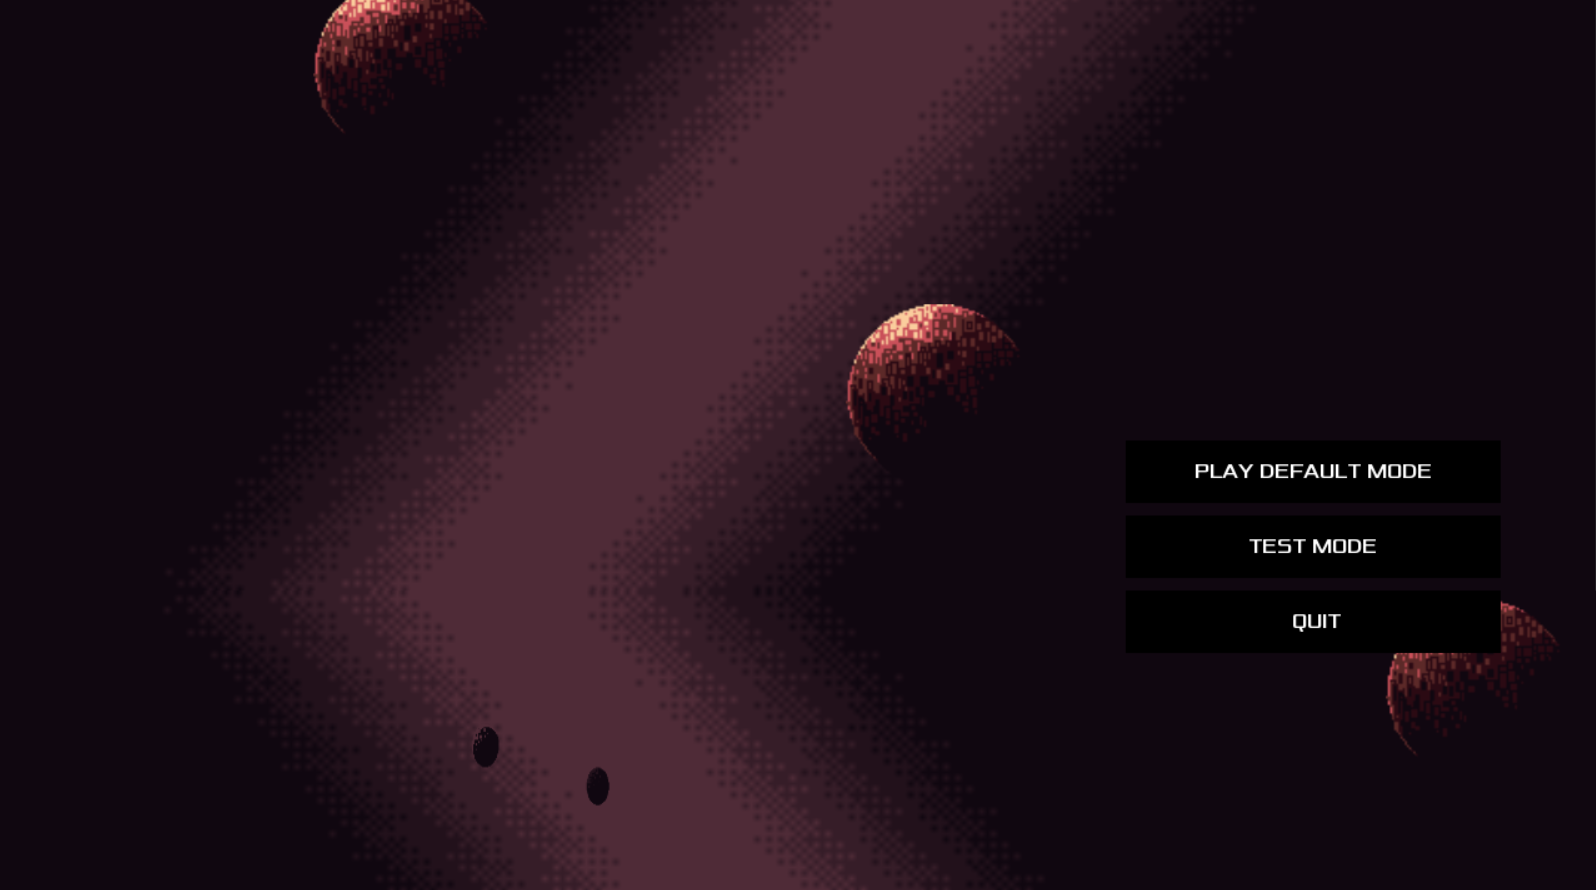
\includegraphics[width=.8\textwidth]{ss/Menu_SS.png}
  \caption{Tela de Teste Space Shooter. Imagem retirada do próprio jogo.\label{fig:tela-de-teste-space-shooter}}
\end{figure}


O menu \textit{Test Mode} permite escolher as configurações necessárias para a execução de um teste, com condições específicas e pré-definidas para obtenção de dados sobre as ondas geradas e o dano total produzido, o menu \textit{Test Mode} de cada jogo encontram-se nas Figuras \ref{fig:td-testes} e  \ref{fig:ss-testes}.

O algoritmo genético foi testado (opção \textit{AI} no menu), em conjunto com opções ingênuas nos dois jogos, posto que foram implementadas para ser comparadas com as ondas geradas pelo algoritmo desenvolvido, em vista de observar se seu desempenho. Assim há opções, apresentadas nas Figuras \ref{fig:td-testes} e \ref{fig:ss-testes} onde as ondas podem ser geradas:
\begin{itemize}
  \item Aleatoriamente - \textit{RANDOM}
  \item Um de cada oponente - \textit{ONE EACH}
  \item Modos "repetição", onde todo inimigo é do mesmo tipo
\end{itemize}

\begin{figure}
  \centering
  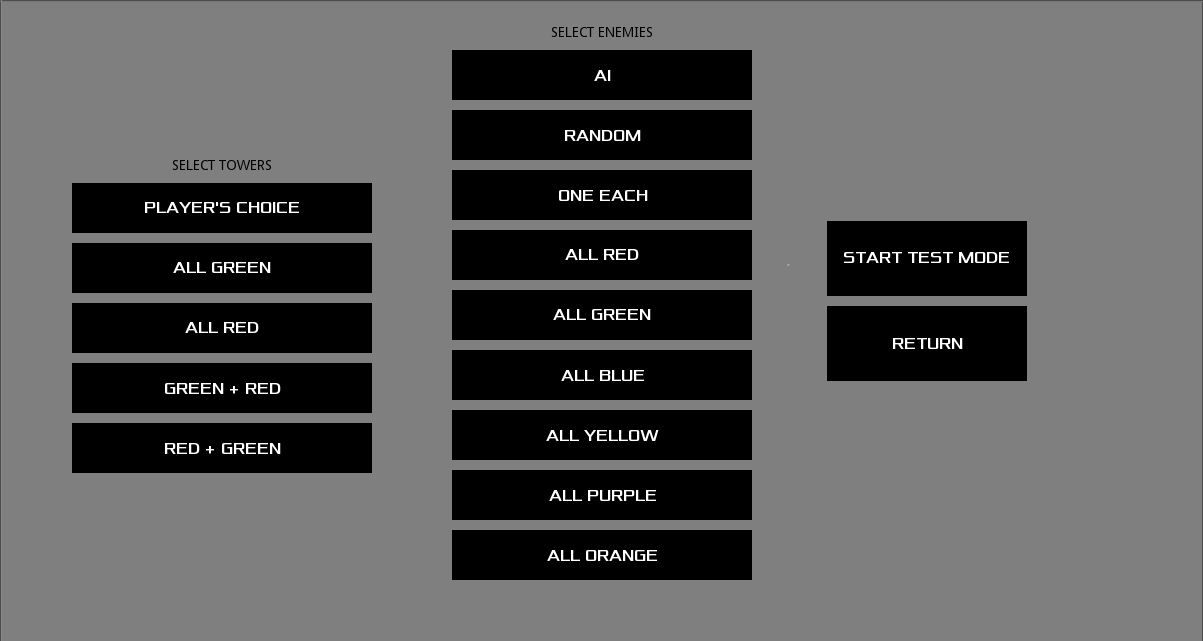
\includegraphics[width=.8\textwidth]{figuras/td/Menu_Escolhas_TESTE_TDD.PNG}
  \caption{Menu de testes Tower Defense. Imagem retirada do próprio jogo.\label{fig:td-testes}}
\end{figure}


\begin{figure}
  \centering
  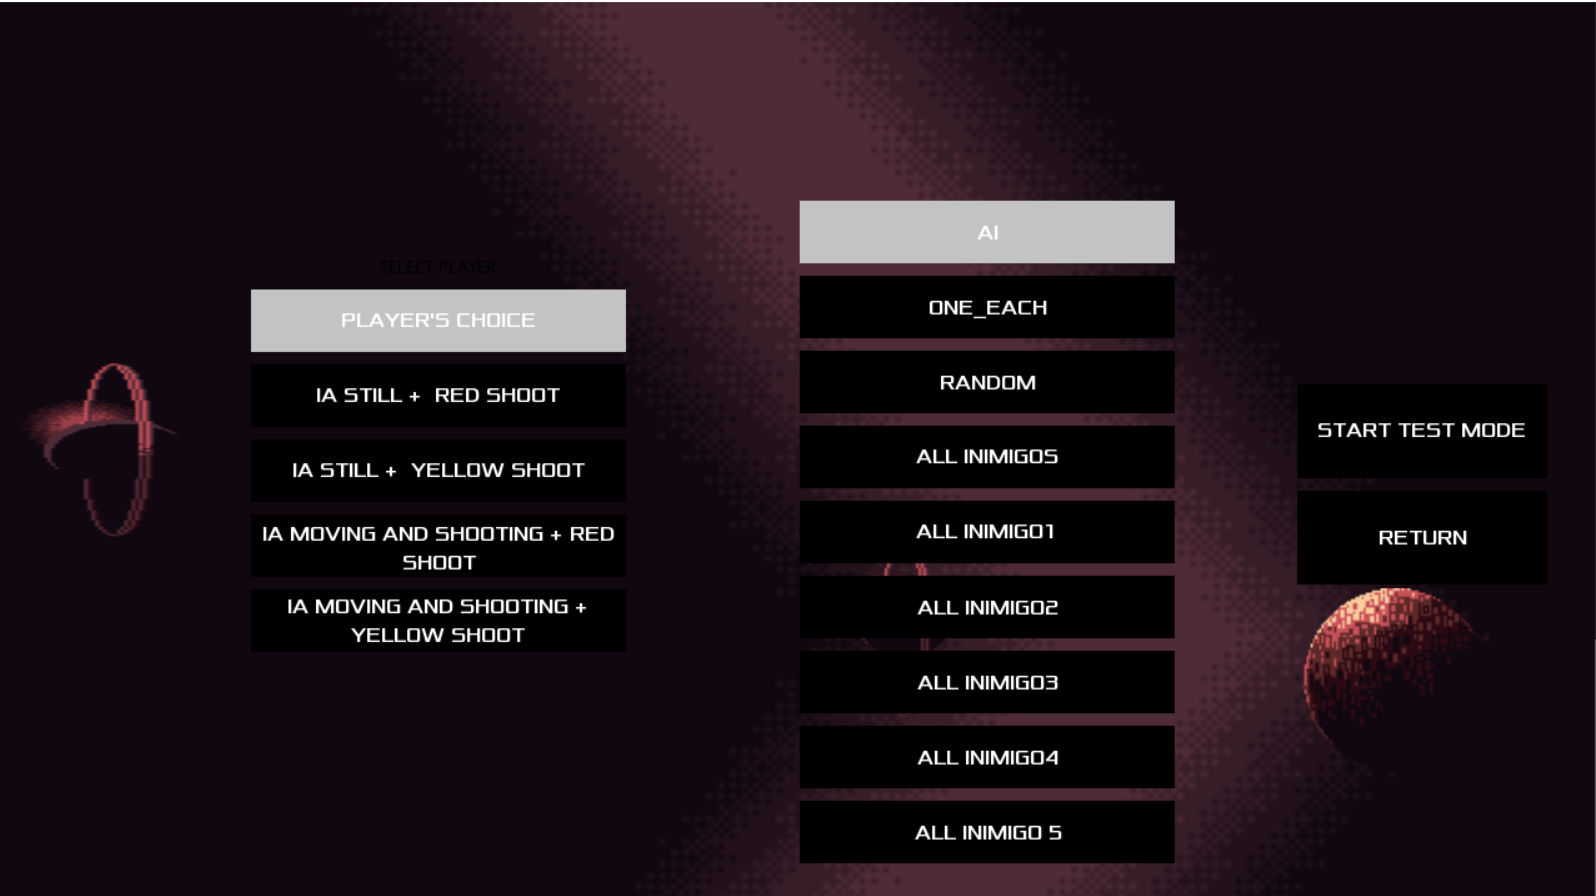
\includegraphics[width=.9\textwidth]{ss/Tela de testes_SS.png}
  \caption{Menu de Testes Space Shooter. Imagem retirada do próprio jogo.\label{fig:ss-testes}}
\end{figure}

\pagebreak

%% ------------------------------------------------------------------------- %%
\subsection{Tower Defense}
\label{sec:mt-td}

No \textit{Tower Defense}, as ondas repetidas enviam 6 inimigos iguais para cada rota norte e sul, um exemplo de uma onda repetida encontra-se na Figura \ref{fig:td-testes-orange} seguindo as rotas que foram já definidas conforme a Figura \ref{fig:td-rota}. Cada onda repetida envia o mesmo tipo de tanque, cujos atributos estam disponíveis na Tabela \ref{tab:tank-dmg2}. O modo \textit{One Each} utiliza os 6 tipos em cada rota; e o \textit{Random} aleatoriza completamente a escolha de tipo e rota, utilizando \textit{RandomNumberGenerator} disponibilizada pela \textit{Godot Engine}. Os modos \textit{Random} e \textit{One Each} podem ser vistos nas Figuras \ref{fig:tdd-testes} e \ref{fig:td-testes-one-each}. 


\begin{figure}
  \centering
  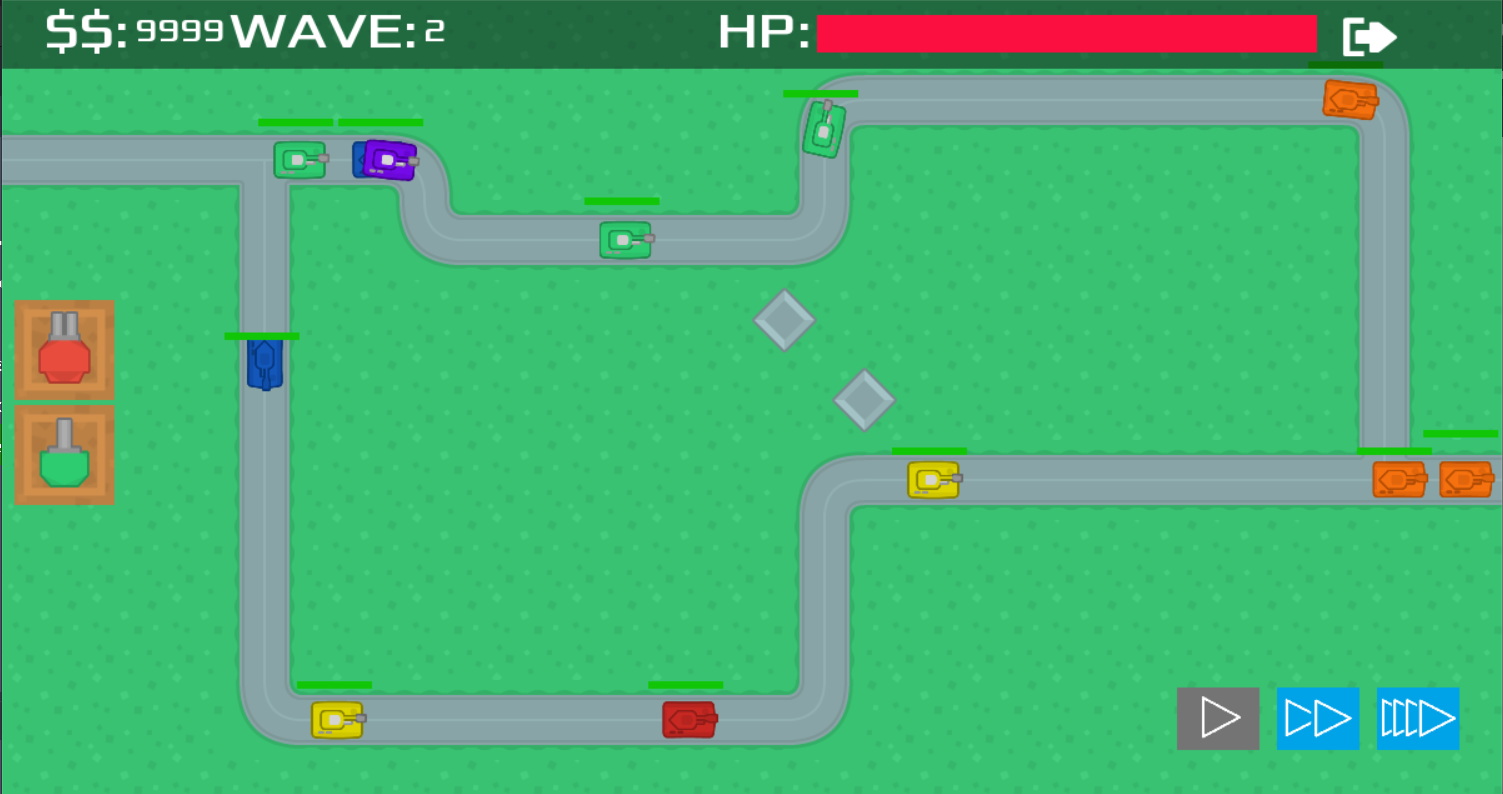
\includegraphics[width=.9\textwidth]{td/Random Mode_TDD Teste.PNG}
  \caption{Escolha Random em tower defense. Imagem retirada do próprio jogo.\label{fig:tdd-testes}}
\end{figure}


\begin{figure}
  \centering
  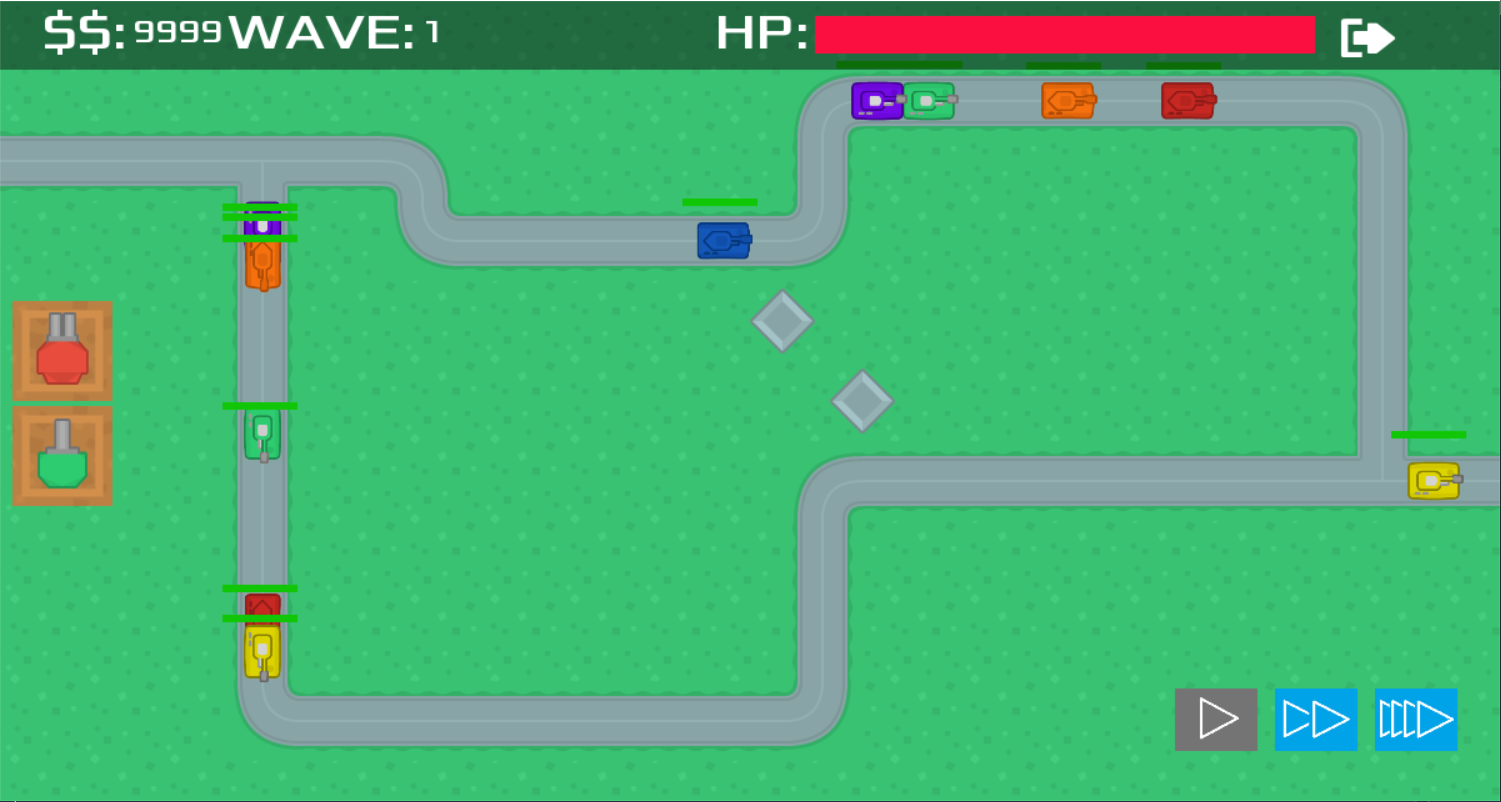
\includegraphics[width=.9\textwidth]{td/Exempleo TDD One EACH.PNG}
  \caption{Escolha One Each no Tower Defense. Imagem retirada do próprio jogo.\label{fig:td-testes-one-each}}
\end{figure}


\begin{figure}
  \centering
  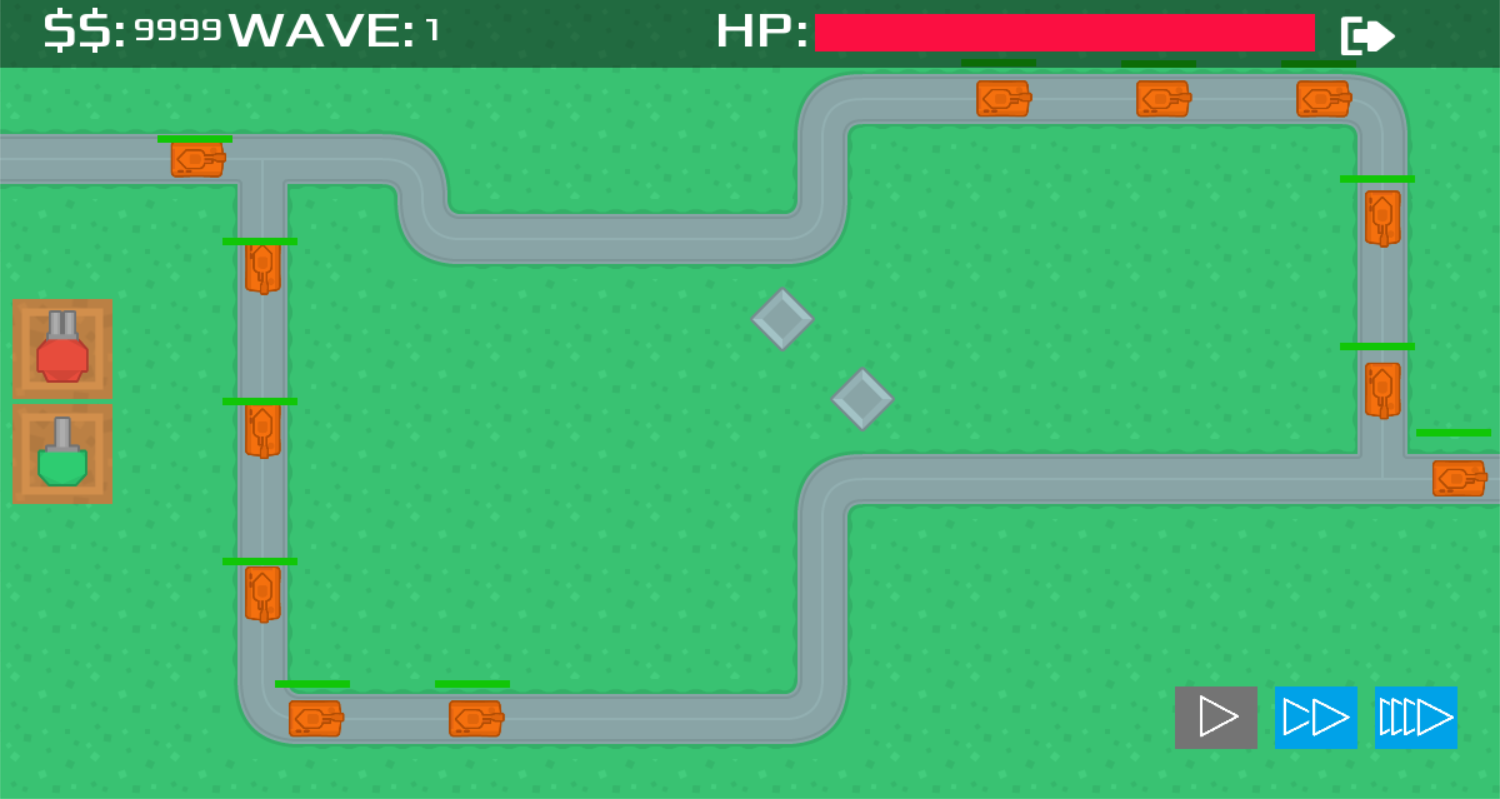
\includegraphics[width=.9\textwidth]{td/Tdd_All_orange.PNG}
  \caption{Opção All Orange. Imagem retirada do próprio jogo.\label{fig:td-testes-orange}}
\end{figure}

\pagebreak

Para uniformizar o comportamento do jogador, as torres foram configuradas para melhor controle dos testes, posicionadas duas por rota, onde o alcance das mesmas fica restrito a somente seu caminho, de maneira a alcançar um balanço entre eliminação e sobrevivência de alguns oponentes, visto as torres terem diferentes valores atribuídos com relação a dano e alcance, presentes na Tabela \ref{tab:dados_torres2}. Assim são geradas 4 configurações de teste, demonstradas nas Figuras \ref{fig:td-teste-all-green}, \ref{fig:tdd-teste-all-red}, \ref{fig:tdd-teste-greenred}, \ref{fig:td-teste-red-green}.

\begin{table}
\caption{Dano das torres no Tower Defense.\label{tab:dados_torres2}}
\begin{tabular}{c|ccc}

             & velocidade de tiro  & dano & alcance\\ \hline
Torre Verde   & 55     & 25     &  350 \\
Torre Vermelha     & 70     & 15     &  550       

\end{tabular}
\end{table}


\begin{table}
\caption{Dano de cada tanque no Tower Defense}
\begin{tabular}{c|cc}
            & velocidade & dano   \\ \hline
tank blue   & 55    & 55         \\
tank green  & 70    & 45         \\
tank red    & 80    & 15          \\
tank orange & 120   & 5           \\
tank purple & 90    & 15          \\
tank yellow & 150   & 5           
\end{tabular}
\label{tab:tank-dmg2}
\end{table}

\pagebreak

\begin{figure}
  \centering
  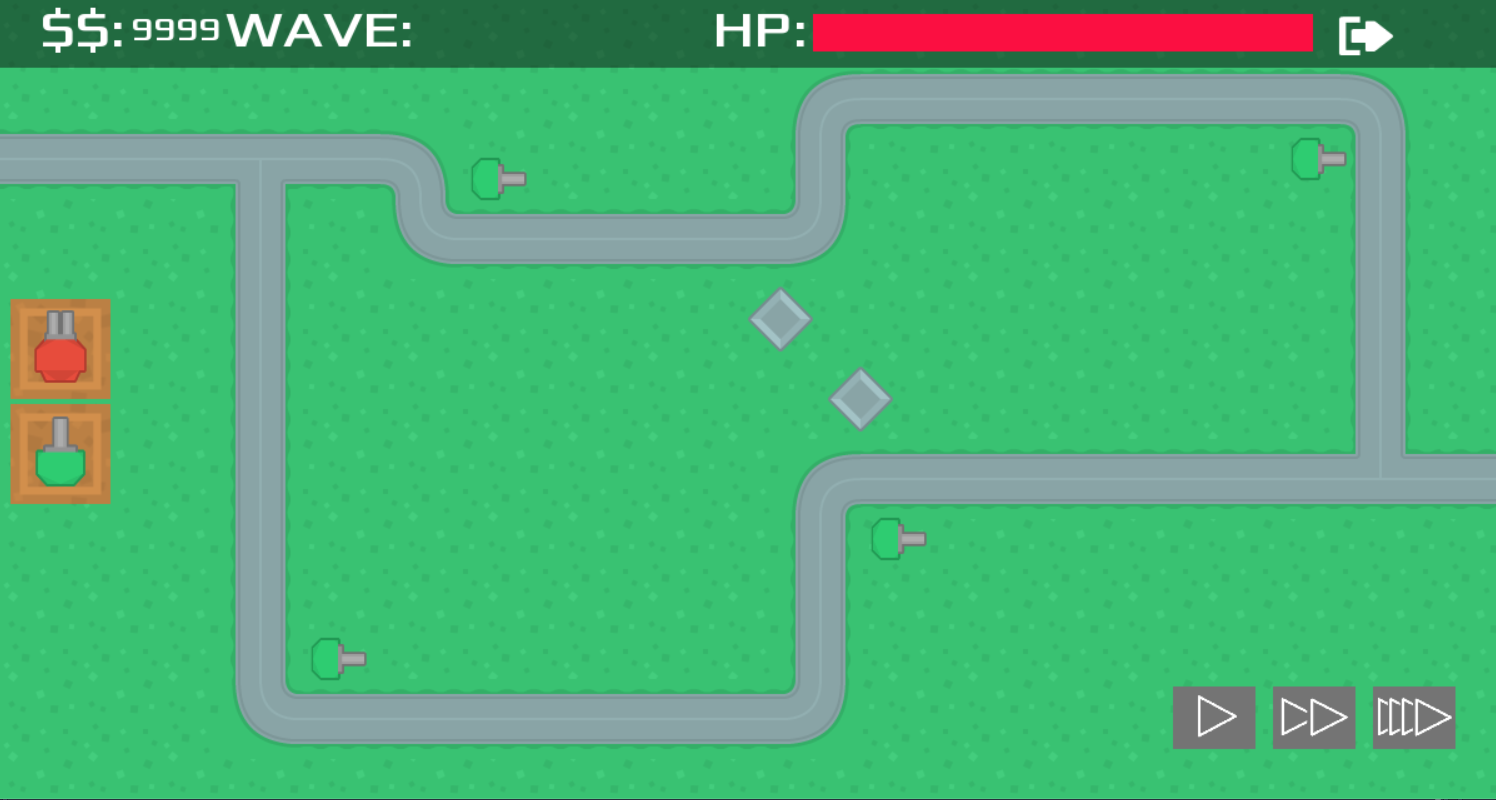
\includegraphics[width=.9\textwidth]{td/Tdd_all_green_teste.png}
  \caption{Teste de torres verdes\label{fig:td-teste-all-green}}
\end{figure}

\begin{figure}
  \centering
  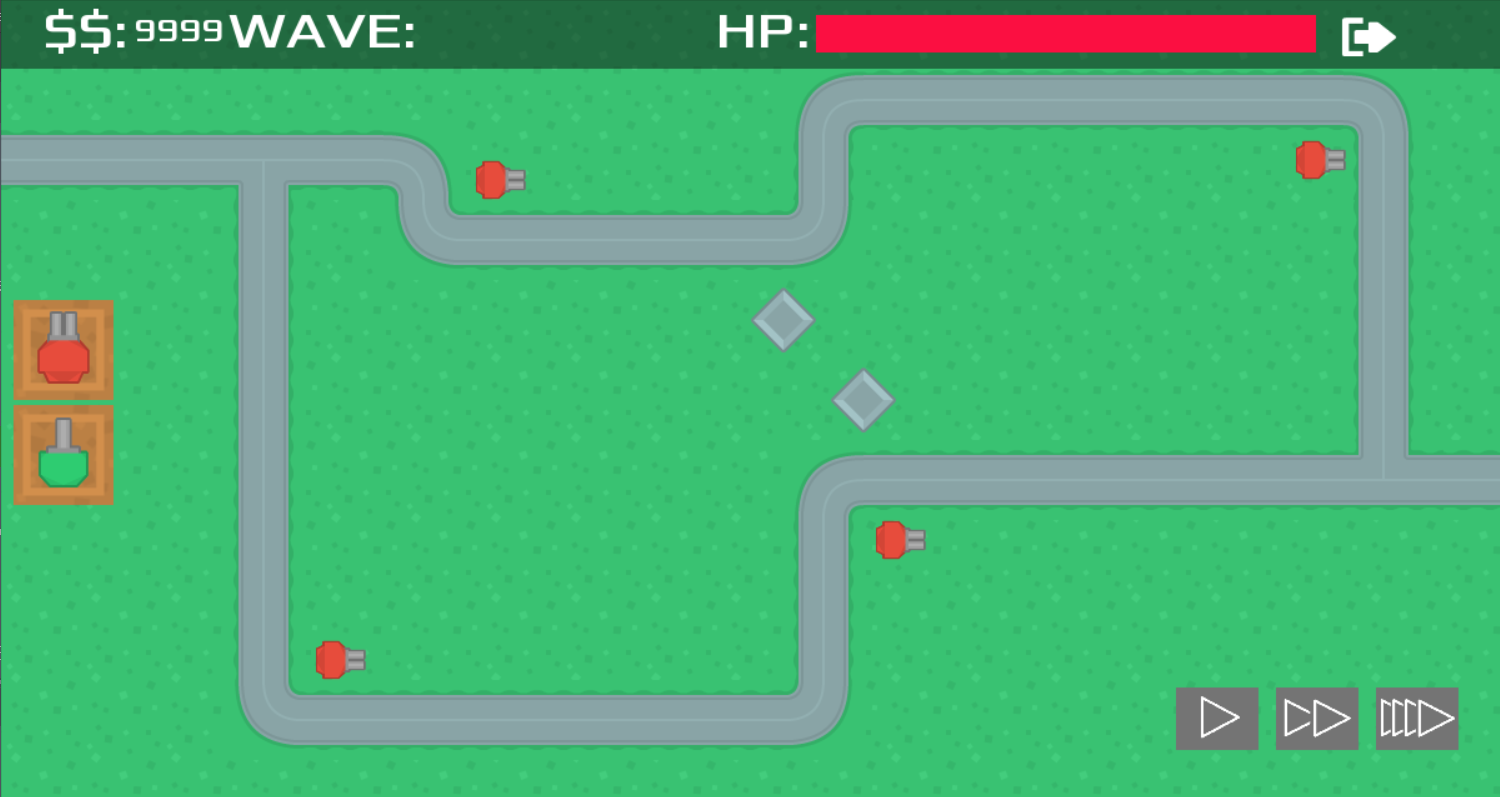
\includegraphics[width=.9\textwidth]{td/ALL RED TDD.png}
  \caption{Teste de torres vermelhas\label{fig:tdd-teste-all-red}}
\end{figure}

\begin{figure}
  \centering
  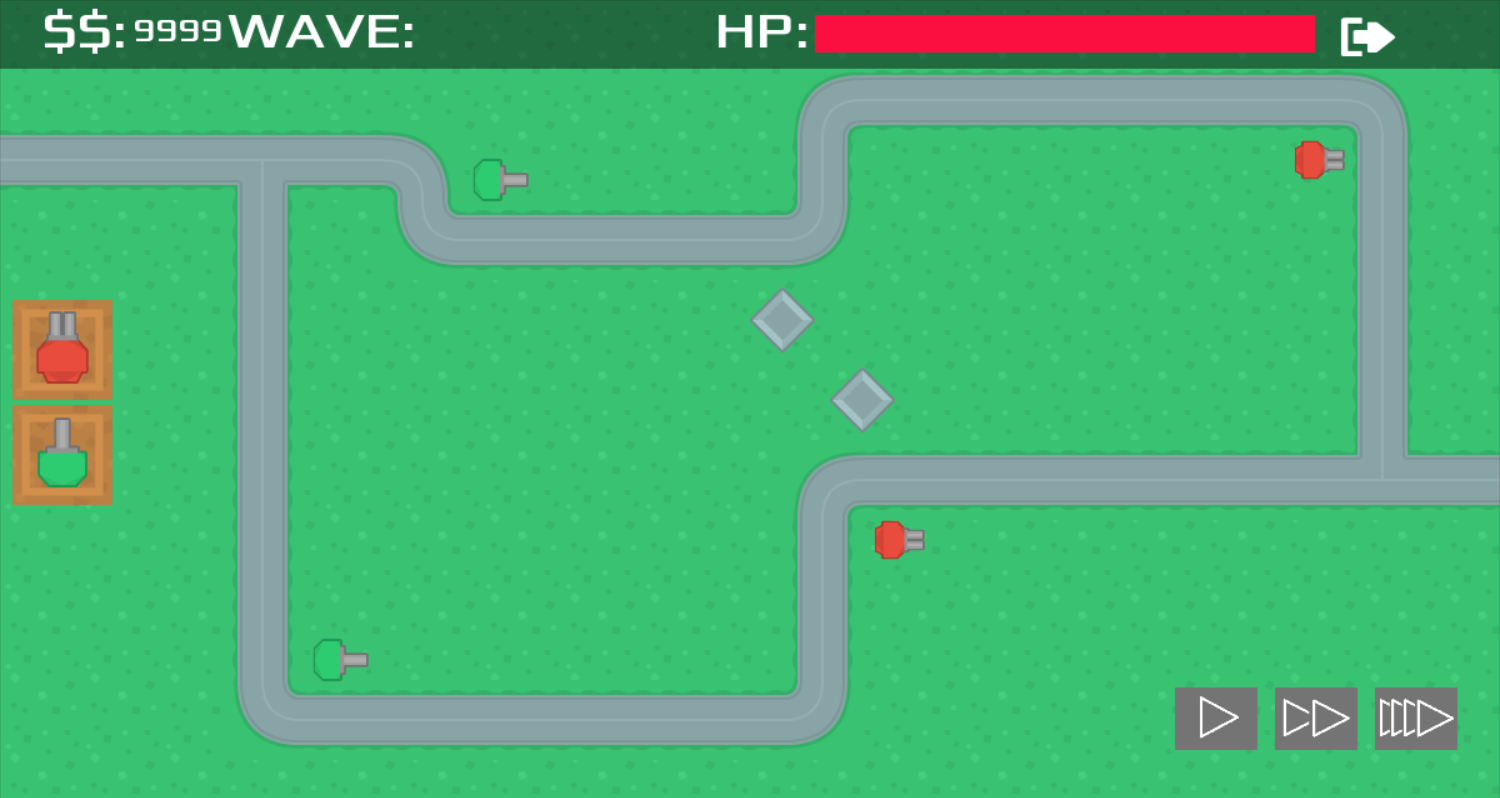
\includegraphics[width=.9\textwidth]{td/Green_Red_TDD.png}
  \caption{Teste de torres verdes com vermelhas\label{fig:tdd-teste-greenred}}
\end{figure}

\begin{figure}
  \centering
  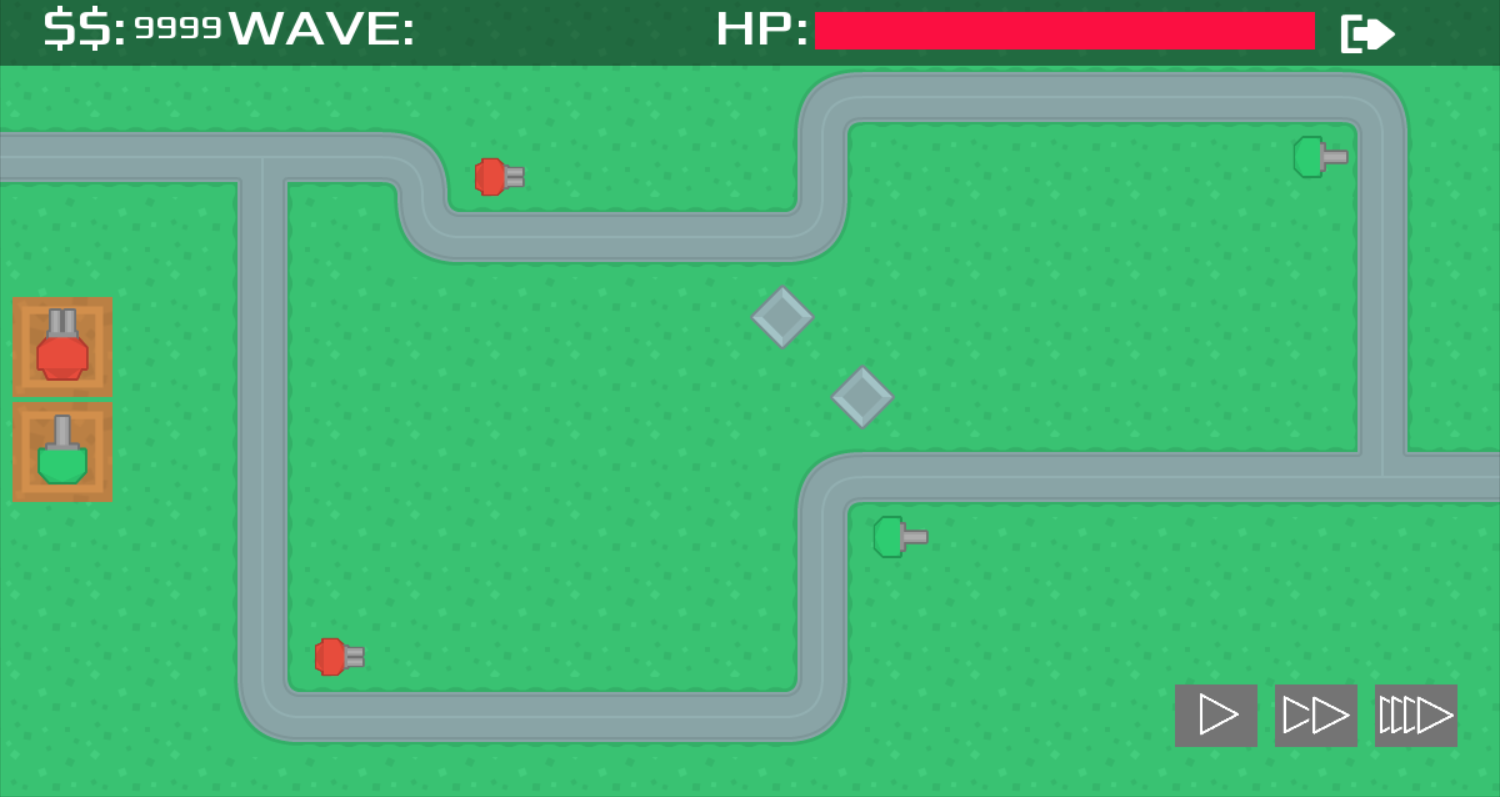
\includegraphics[width=.9\textwidth]{td/RED_GREEN TDD.png}
  \caption{Teste de torres vermelhas com verdes\label{fig:td-teste-red-green}}
\end{figure}

\newpage
%% ------------------------------------------------------------------------- %%
\subsection{Space Shooter}
\label{sec:mt-ss}

O \textit{Space Shooter} foi configurado de maneira próxima do \textit{Tower Defense}, mas foi preservada a capacidade dos asteroides aparecerem em locais aleatórios entre os 6 possíveis do jogo, exceto quando a IA está gerando os inimigos, onde o algoritmo busca o melhor \textit{spawn}. As naves foram alteradas para efetivamente jogarem a partida; com um nó \textit{Area2D} ao seu redor para detecção e ataque contra o primeiro inimigo que colidir contra o nó, conforme a Figura \ref{fig:ss-area}; e com a implementação de uma opção de movimentação, visto a Figura \ref{fig:ss-move}, permitindo testes com uma nave estática no centro da tela, e com movimentação lateral, de lado a lado, pausando nas extremidades.

\begin{figure}
  \centering
  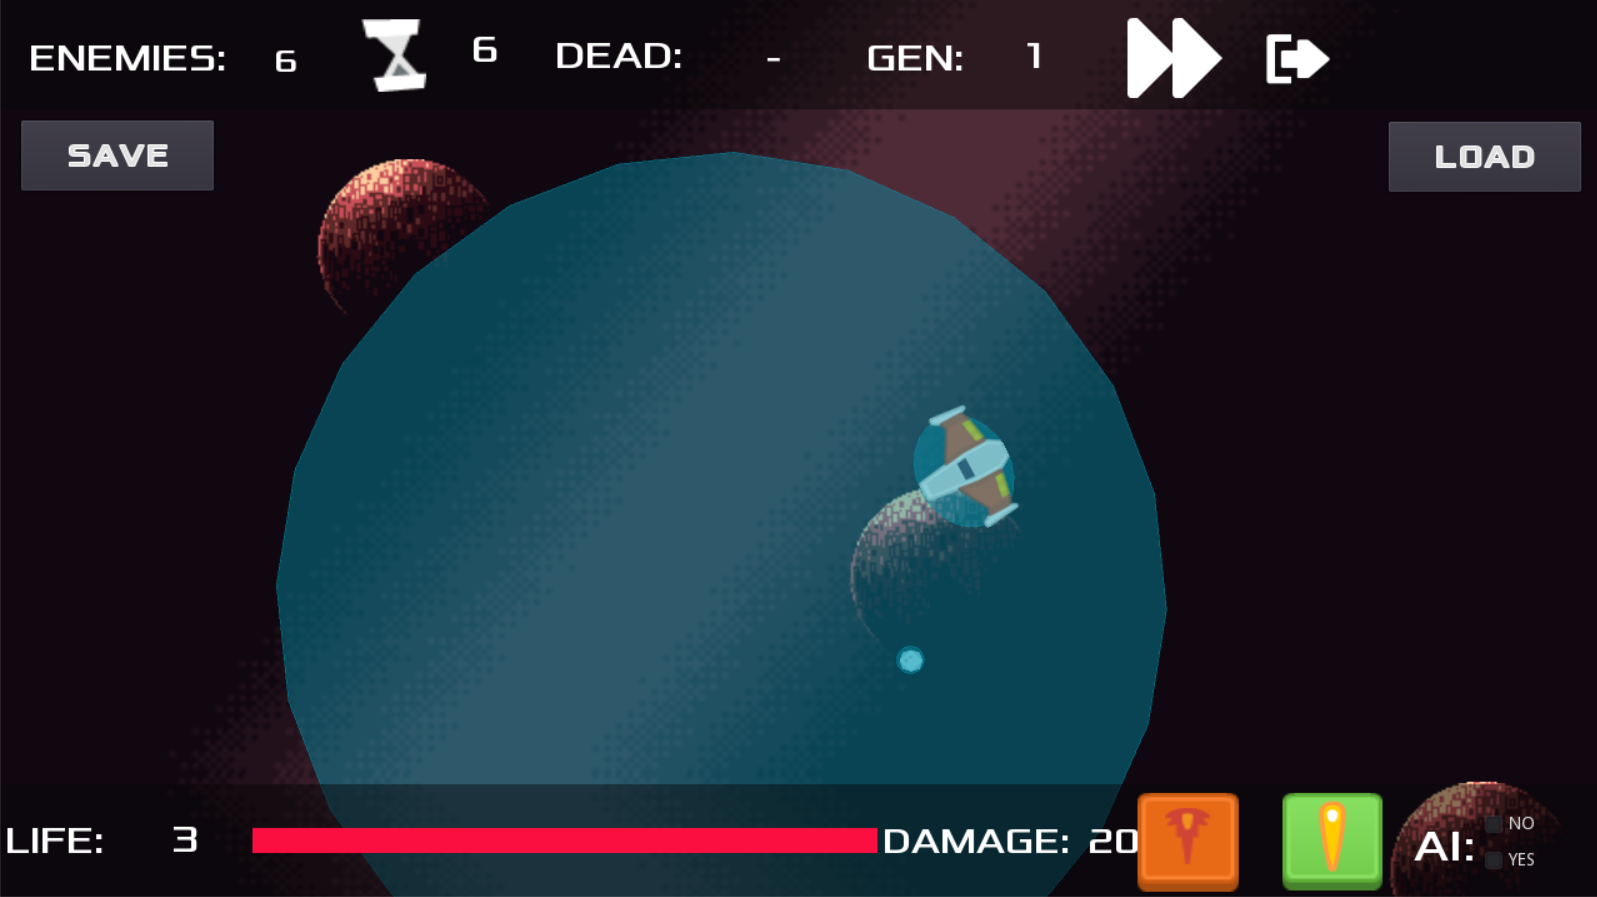
\includegraphics[width=.9\textwidth]{ss/Area de deteccao_Player_IA_jogo_exemplo.png}
  \caption{Área de detecção da nave em um modo de teste. Imagem retirada do próprio jogo.\label{fig:ss-area}}
\end{figure}

\begin{figure}
  \centering
  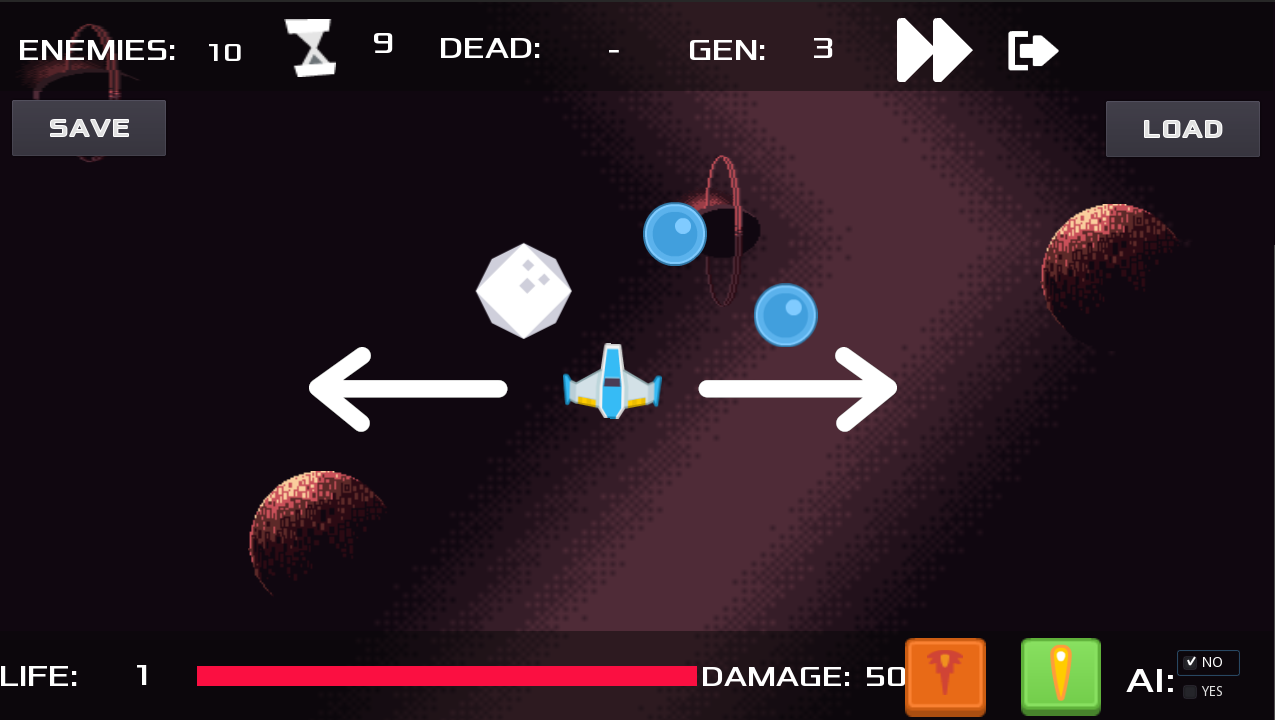
\includegraphics[width=.9\textwidth]{ss/ss_move.png}
  \caption{Movimentação da nave em um modo de teste. Imagem retirada do jogo e editada.\label{fig:ss-move}}
\end{figure}

\pagebreak

As opções dos inimigos são semelhantes ao \textit{Tower Defense}, com ondas sempre com os mesmos inimigos, ou um de cada, ou escolhendo aleatoriamente através do \textit{RandomNumberGenerator} da \textit{engine}. Reiterando que nestes casos o \textit{spawn} dos asteroides ocorre em qualquer um dos 6 locais disponíveis na Figura \ref{fig:ss-positions} escolhidos de maneira aleatória pelo jogo.
\par

%!TeX root=../tese.tex
%("dica" para o editor de texto: este arquivo é parte de um documento maior)
% para saber mais: https://tex.stackexchange.com/q/78101/183146

%% ------------------------------------------------------------------------- %%
\chapter{Apresentação dos Resultados}
\label{cap:apresentacao}

Para determinar a efetividade do algoritmo genético, foram utilizados métodos estatísticos para comparar o desempenho do mesmo contra outros mecanismos de geração de oponentes. Para aproveitar melhor as características determinísticas do jogo \textit{Tower Defense}, os experimentos se concentraram no mesmo, pois a natureza mais aleatória do \textit{Space Shooter} produziu resultados mais difíceis de analisar e, infelizmente, não havia mais tempo disponível para ajustar os cenários e função \textit{fitness} ou taxa de mutação até encontrar resultados mais conclusivos.

%% ------------------------------------------------------------------------- %%
\section{Organização dos dados}
\label{sec:a-organizacao}

A análise dos dados partiu das estatísticas descritivas de cada onda para todos os experimentos executados, conforme ilustrado pela Tabela \ref{tab:colunas}; isto é, foram obtidos 30 amostras de dano para cada i-ésima onda.

\begin{table}
\caption{Forma de coleta dos dados de cada onda.}
\begin{tabular}{l|l|l|l|l|l|l}
\cline{2-6}
               & onda 1 & onda 2 & ... & onda n - 1 & onda n \\ \cline{2-6}
experimento 1  &        &        &     &            &         \\
experimento 2  &  dano  &  dano  &     &  dano      &  dano   \\
...            &  da    &  da    & ... &  da        &  da     \\
experimento 29 &  onda  &  onda  &     &  onda      &  onda   \\
experimento 30 &        &        &     &            &         \\ \cline{2-6}
\end{tabular}
\label{tab:colunas}
\end{table}

%% ------------------------------------------------------------------------- %%
\section{Dados das Ondas}
\label{sec:a-ondas}

As seções seguintes irão dispor os dados considerados relevantes para análise de desempenho do algoritmo, obtidos através da análise exploratória de dados pelos \textit{Jupyter Notebook}\footnote{Repositório disponível em \url{https://github.com/raktanaka/tcc-results} - 24/12/2021} desenvolvidos. Dados de ondas sempre com o mesmo tipo de inimigos - chamadas de ondas repetidas - podem mostrar uma possível solução maximal ou próxima dela, para a qual o algoritmo poderia convergir. Já os dados de ondas com inimigos escolhidos ao acaso - chamadas de ondas aleatórias - indicam um possível valor de dano mínimo, que seria atingido com um método que também não precisa de conhecimento das mecânicas de jogo e de informações sobre os inimigos disponibilizadas.

Para visualização do funcionamento dos algoritmos, foram geradas imagens com as modas\footnote{Valores mais frequentes em um conjunto de dados} das ondas geradas a partir dos arquivos de texto com os dados. Um \textit{notebook} faz os cálculo necessários e utiliza a biblioteca \textit{Matplotlib} para produzir a imagem com os \textit{sprites} e caminho ou localização do inimigo. As figuras fornecem os inimigos mais comuns em cada onda, mostrando para qual solução o algoritmo tende a convergir. Estas estão disponíveis nos apêndices \ref{sec:apend-moda-td-v1}, \ref{sec:apend-moda-td-v2}, \ref{sec:apend-moda-td-v3}, \ref{sec:apend-moda-ss-v1}, \ref{sec:apend-moda-ss-v3}.

%% ------------------------------------------------------------------------- %%
\subsection{Tower Defense - Ondas Repetidas}
\label{sec:uni-td}

Seguem os dados obtidos nos experimentos feito no jogo, para facilidade de leitura, uma cópia da tabela \ref{tab:tank-dmg} da seção \ref{sec:mj-td} está abaixo.

\begin{table}
\caption{Dano de cada tanque no Tower Defense}
\begin{tabular}{c|cc}
            & velocidade & dano   \\ \hline
tank blue   & 55    & 55         \\
tank green  & 70    & 45         \\
tank red    & 80    & 15          \\
tank orange & 120   & 5           \\
tank purple & 90    & 15          \\
tank yellow & 150   & 5           
\end{tabular}
\label{tab:tank-dmg3}
\end{table}

Através da Tabela \ref{tab:tank-dmg3} é possível calcular o dano máximo possível como produto dos 12 inimigos que podem ser gerados por \textit{wave} e do maior dano disponível:
\[12 * 55 = 660\]
Numa onda composta inteiramente por tanques verdes (\textit{EnemyGreen}), sem nenhuma eliminação. As Tabelas \ref{tab:green}, \ref{tab:red}, \ref{tab:greenred} e \ref{tab:redgreen} a seguir mostram os dados de dano médio para cada onda e cada tipo de inimigo, obtidos através das simulações do jogo.

\begin{table}
\caption{Desempenho das \textbf{ondas repetidas} contra Torres \textbf{exclusivamente Verdes}}
\begin{tabular}{l|l|ll}
Torres & Inimigos & Dano Médio & Desvio Padrão \\ \hline
Verdes & EnemyGreen    & 450.00     & 0.0           \\
Verdes & OneEach       & 122.35     & 4.52          \\
Verdes & EnemyPurple   & 90.06      & 0.91          \\
Verdes & EnemyRed      & 89.90      & 1.22          \\
Verdes & EnemyBlue     & 60.68      & 16.77         \\
Verdes & EnemyYellow   & 40.07      & 0.57          \\
Verdes & EnemyOrange   & 39.93      & 0.57         
\end{tabular}
\label{tab:green}
\end{table}

Conforme os dados gerados para torres exclusivamente verdes, nota-se que tanques verdes possuem maior facilidade em causar dano ao jogador, uma vez que possuem a mecânica de \textbf{Resistência} contra torres da mesma cor que eles. Portanto, no algoritmo genético, espera-se que esses sejam os indivíduos mais numerosos da população final.

\begin{table}
\caption{Desempenho das \textbf{ondas repetidas} contra Torres \textbf{exclusivamente Vermelhas}}
\begin{tabular}{l|l|ll}
Torres    & Inimigos & Dano Médio & Desvio Padrão \\ \hline
Vermelhas & EnemyGreen    & 360.00     & 0.0           \\
Vermelhas & EnemyBlue     & 355.85     & 28.58         \\
Vermelhas & EnemyRed      & 180.00     & 0.0           \\
Vermelhas & OneEach       & 167.82     & 2.48          \\
Vermelhas & EnemyPurple   & 127.60     & 8.54          \\
Vermelhas & EnemyYellow   & 50.58      & 1.61          \\
Vermelhas & EnemyOrange   & 50.00      & 0.0          
\end{tabular}
\label{tab:red}
\end{table}

Os dados gerados para torres exclusivamente vermelhas apresenta que, em média,  tanques Verdes e Azuis são os melhores causadores de dano por onda, mesmo com a resistência dos tanques vermelhos sobre as torres vermelhas. Essa disparidade ocorre pela quantidade de dano que os tanques causam ao chegar no inimigo, conforme Tabela \ref{tab:tank-dmg3}, o tanque vermelho causa 15 de dano, ou seja, os 12 ($\frac{180}{15}$) tanques sobrevivem ao final de todas as ondas. Contudo, os inimigos verdes e azuis causam mais dano, mesmo que cheguem menos tanques ao final do trajeto, 8 ($\frac{360}{45}$) para tanques verdes e entre 6-7 ($\frac{355}{55}$) nos azuis. 

\begin{table}
\caption{Desempenho das \textbf{ondas repetidas} contra \textbf{1 Torre Verde e 1 Vermelha} (Nessa ordem)}
\begin{tabular}{l|l|ll}
Torres           & Inimigos & Dano Médio & Desvio Padrão \\ \hline
Verde + Vermelha & EnemyGreen    & 420.20     & 13.91         \\
Verde + Vermelha & EnemyBlue     & 220.18     & 3.18          \\
Verde + Vermelha & EnemyRed      & 148.50     & 4.50          \\
Verde + Vermelha & OneEach       & 148.45     & 4.57          \\
Verde + Vermelha & EnemyPurple   & 120.00     & 0.0           \\
Verde + Vermelha & EnemyYellow   & 50.00      & 0.0           \\
Verde + Vermelha & EnemyOrange   & 44.50      & 1.50          
\end{tabular}
\label{tab:greenred}
\end{table}

\pagebreak

Conforme as informações da Tabela \ref{tab:greenred}, percebe-se que o inimigo Verde tem o melhor desempenho de dano por onda repetida, mesmo que sobrevivam menos indivíduos ao final em comparação ao inimigo Vermelho, uma vez que o dano de Verde é 3 vezes maior. Chegam ao final, aproximadamente 9 ($\frac{420}{45}$) Verdes e 10 Vermelhos ($\frac{148.5}{15}$). 

\begin{table}[H]
\caption{Desempenho das \textbf{ondas repetidas} contra \textbf{1 Torre Vermelha e 1 Verde}(Nessa ordem)}
\begin{tabular}{l|l|ll}
Torres            & Inimigos & Dano Médio & Desvio Padrão \\ \hline
Vermelha + Verde  & EnemyGreen      & 449.85     & 2.60          \\
Vermelha + Verde  & EnemyBlue       & 329.82     & 3.18          \\
Vermelha + Verde  & EnemyRed        & 149.90     & 1.73          \\
Vermelha + Verde  & OneEach         & 135.05     & 0.87          \\
Vermelha + Verde  & EnemyPurple     & 120.00     & 0.0           \\
Vermelha + Verde  & EnemyYellow     & 50.00      & 0.0           \\
Vermelha + Verde  & EnemyOrange     & 49.45      & 1.57          
\end{tabular}
\label{tab:redgreen}
\end{table}

Para a Tabela \ref{tab:redgreen}, nota-se um aumento de desempenho significativo do inimigo Azul e Verde, onde sobrevive um tanque a mais verde e quase 2 azuis em relação ao anterior. Contudo, mantém-se a dominância do dano médio por onda do inimigo Verde. Os desvios padrões baixos - o mais alto apresentado nas Torres Verdes contra \textit{EnemyBlue} é de aproximadamente 25\% do dano total, mas é uma exceção considerando todos os resultados - mostram a consistência do jogo.

Conforme os dados gerados, o inimigo Verde indica ter o melhor desempenho de dano nas ondas repetidas, contudo, mais para frente desse capítulo, será mostrado que eles não serão os mais selecionados, por conta da função \textit{fitness} escolhida, que prioriza sobrevivência ao invés de dano por \textit{wave}.

%% ------------------------------------------------------------------------- %%
\subsection{Tower Defense - Ondas Aleatórias}
\label{sec:rd-td}

Foram calculadas as médias de dano causadas por cada onda aleatória de distribuição uniforme (Tabela \ref{tab:td-rd-avg}) e o máximo de dano causado em qualquer onda (Tabela \ref{tab:td-rd-max}), considerando todos os experimentos. A Figura \ref{fig:td-rd-max} ilustra a onda que causou o maior dano.

\begin{table}
\begin{tabular}{l|ll}
Torres            & Dano Médio & Desvio Padrão \\ \hline
Verdes            & 81.42      & 55.00         \\
Vermelhas         & 125.35     & 56.98         \\
Verde + Vermelha  & 100.37     & 54.16         \\
Vermelha + Verde  & 102.37     & 56.62          
\end{tabular}
\caption{Média e Desvio Padrão do dano em ondas aleatórias no Tower Defense.}
\label{tab:td-rd-avg}
\end{table}

\pagebreak

\begin{table}
\centering
\begin{tabular}{p{1.7cm}|l|p{1.0cm}}
Torres                   & Onda                                                                                                                         & Dano \newline Total \\ \hline
Verdes                   & \begin{tabular}{@{}c@{}} {[}EnemyGreen, 1{]}; {[}EnemyGreen, 1{]}; {[}EnemyGreen, 0{]}; {[}EnemyRed, 1{]};     \\
                                                    {[}EnemyPurple, 0{]}; {[}EnemyGreen, 0{]}; {[}EnemyRed, 1{]}; {[}EnemyGreen, 0{]};    \\
                                                    {[}EnemyOrange, 0{]}; {[}EnemyGreen, 0{]}; {[}EnemyGreen, 0{]}; {[}EnemyRed, 0{]}     \end{tabular} & 290        \\ \hline
Vermelhas                & \begin{tabular}{@{}c@{}} {[}EnemyBlue, 0{]}; {[}EnemyRed, 0{]}; {[}EnemyBlue, 0{]}; {[}EnemyGreen, 0{]};       \\
                                                    {[}EnemyGreen, 1{]}; {[}EnemyRed, 1{]}; {[}EnemyBlue, 0{]}; {[}EnemyOrange, 1{]};     \\
                                                    {[}EnemyBlue, 0{]}; {[}EnemyYellow, 0{]}; {[}EnemyOrange, 0{]}; {[}EnemyYellow, 1{]}  \end{tabular} & 355        \\ \hline
Verde + \newline Vermelha & \begin{tabular}{@{}c@{}} {[}EnemyPurple, 0{]}; {[}EnemyBlue, 0{]}; {[}EnemyBlue, 0{]}; {[}EnemyBlue, 1{]};    \\
                                                     {[}EnemyRed, 0{]}; {[}EnemyGreen, 1{]}; {[}EnemyYellow, 0{]}; {[}EnemyRed, 1{]};     \\
                                                     {[}EnemyGreen, 1{]}; {[}EnemyGreen, 0{]}; {[}EnemyGreen, 0{]}; {[}EnemyYellow, 1{]}  \end{tabular} & 330        \\ \hline
Vermelha \newline + Verde & \begin{tabular}{@{}c@{}} {[}EnemyYellow, 0{]}; {[}EnemyBlue, 0{]}; {[}EnemyRed, 1{]}; {[}EnemyGreen, 0{]};    \\
                                                     {[}EnemyGreen, 1{]}; {[}EnemyRed, 1{]}; {[}EnemyGreen, 0{]}; {[}EnemyYellow, 0{]};   \\
                                                     {[}EnemyRed, 1{]}; {[}EnemyGreen, 0{]}; {[}EnemyGreen, 0{]}; {[}EnemyPurple, 1{]}    \end{tabular} & 315       
\end{tabular}
\caption{Ondas aleatórias com maior dano no Tower Defense.}
\label{tab:td-rd-max}
\end{table}

\begin{figure}
  \centering
  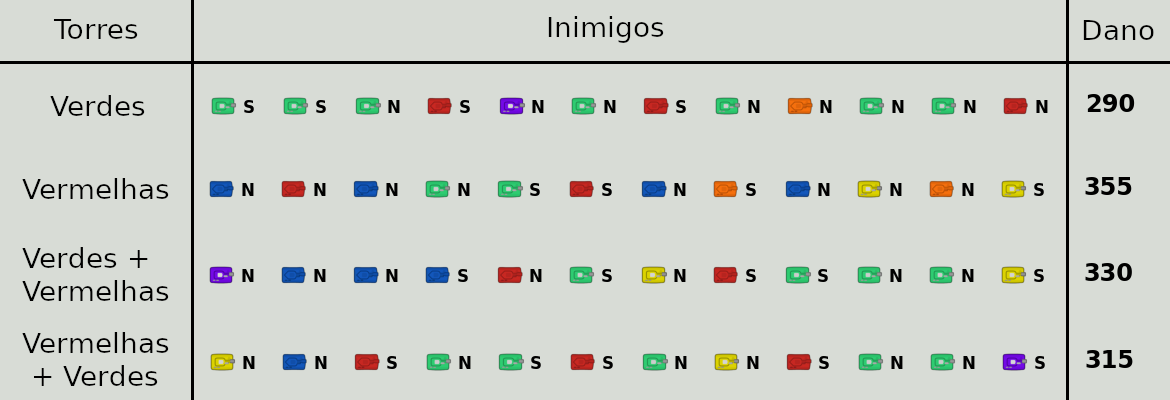
\includegraphics[width=1.0\textwidth]{td/tab-rd-max.png}
  \caption{Visualização das ondas aleatórias com maior dano no Tower Defense.}
  \label{fig:td-rd-max}
\end{figure}

%% ------------------------------------------------------------------------- %%
\subsection{Space Shooter - Ondas Repetidas}
\label{sec:uni-ss}


Foram executados experimentos análogos ao \textit{Tower Defense} no \textit{Space Shooter}, segue uma cópia da tabela \ref{tab:ss-ast-dmg} da seção \ref{sec:mj-ss} para facilitar leitura.

\begin{table}[H]
\caption{Velocidade, dano e vida de cada asteroide no Space Shooter}
\begin{tabular}{c|ccc}
         & Velocidade & Dano & Vida   \\ \hline
inimigos & 500        & 20     &   50     \\
inimigo1 & 350        & 45     &   30     \\
inimigo2 & 470        & 50     &   40     \\
inimigo3 & 320        & 60     &   40     \\
inimigo4 & 550        & 20     &   60     \\
inimigo5 & 700        & 10     &   120      
\end{tabular}
\label{tab:ss-ast-dmg-copia}
\end{table}

\pagebreak

Através da Tabela \ref{tab:ss-ast-dmg-copia}, é possível calcular o dano máximo possível como a onda de seis inimigos com o maior dano disponível:
\[6 * 60 = 360\]
Numa onda composta inteiramente pelo \textit{inimigo3}, sem nenhuma eliminação. As tabelas \ref{tab:ss-yellow-still}, \ref{tab:ss-yellow-move}, \ref{tab:ss-red-still} e \ref{tab:ss-red-move} a seguir mostram os dados de dano médio para cada onda e cada tipo de inimigo.

\begin{table}
\centering
\caption{\textbf{Ondas repetidas} contra IA de \textbf{Disparo Amarelo} e \textbf{Parado}} .
\begin{tabular}{l|l|ll}
Nave                     & Inimigo  & Dano Médio & Desvio Padrão \\ \hline
Disparo Amarelo - Parada & Inimigo3 & 314.93     & 42.46         \\
Disparo Amarelo - Parada & Inimigo2 & 299.78     & 3.33          \\
Disparo Amarelo - Parada & Inimigo1 & 181.50     & 41.67         \\
Disparo Amarelo - Parada & Inimigo4 & 120.00     & 0.0           \\
Disparo Amarelo - Parada & Inimigos & 120.00     & 0.0           \\
Disparo Amarelo - Parada & OneEach  & 82.75      & 27.47         \\
Disparo Amarelo - Parada & Inimigo5 & 60.00      & 0.0          
\end{tabular}
\label{tab:ss-yellow-still}
\end{table}

Na tabela, nota-se que os valores piores classificados são as ondas em que todos os asteroides chegaram no Jogador, mas possuem danos muito baixos ($\frac{\text{dano médio}}{\text{dano individual do asteróide}}$), enquanto os que possuem danos melhores perderam algum indivíduo da população no caminho, pois possuem valores menores que os danos totais possíveis (dano * 6, onde 6 é quantidade de inimigos) e seu desvio padrão é alto.

\begin{table}
\centering
\caption{\textbf{Ondas repetidas} contra IA de \textbf{Disparo Amarelo} e \textbf{Movendo}}.
\begin{tabular}{l|l|ll}
Nave                      & Inimigo  & Dano Médio & Desvio Padrão \\ \hline
Disparo Amarelo - Movendo & Inimigo3 & 213.20     & 52.43         \\
Disparo Amarelo - Movendo & Inimigo2 & 184.61     & 41.98         \\
Disparo Amarelo - Movendo & Inimigo1 & 130.10     & 48.15         \\
Disparo Amarelo - Movendo & OneEach  & 100.85     & 43.75         \\
Disparo Amarelo - Movendo & Inimigo4 & 80.69      & 15.70         \\
Disparo Amarelo - Movendo & Inimigos & 67.69      & 15.46         \\
Disparo Amarelo - Movendo & Inimigo5 & 39.23      & 7.71         
\end{tabular}
\label{tab:ss-yellow-move}
\end{table}

Para esses dados, nota-se que, com a Nave se movendo, a chance dos inimigos acertarem o Jogador decai bastante em todos os casos, contudo, os tipos de inimigos mais promissores ainda se mantém como Inimigo3, Inimigo2 e Inimigo1.

\pagebreak

\begin{table}
\centering
\begin{tabular}{l|l|ll}
Nave                      & Inimigo  & Dano Médio & Desvio Padrão \\ \hline
Disparo Vermelho - Parada & Inimigo3 & 241.60     & 56.01         \\
Disparo Vermelho - Parada & Inimigo2 & 240.94     & 56.09         \\
Disparo Vermelho - Parada & OneEach  & 125.99     & 38.03         \\
Disparo Vermelho - Parada & Inimigo4 & 106.00     & 21.81         \\
Disparo Vermelho - Parada & Inimigos & 102.44     & 20.04         \\
Disparo Vermelho - Parada & Inimigo5 & 62.57      & 17.74         \\
Disparo Vermelho - Parada & Inimigo1 & 27.60      & 29.54        
\end{tabular}
\caption{\textbf{Ondas repetidas} contra IA de \textbf{Disparo Vermelho} e \textbf{Parado} \label{tab:ss-red-still}}.
\end{table}

Para esses dados, percebe-se que o Disparo Vermelho tem uma vantagem muito maior contra \textbf{Inimigo1}, um dos candidatos para o indivíduo mais apto da população nos testes para o Disparo Amarelo, principalmente por matá-lo em um único disparo.

\begin{table}
\centering
\caption{\textbf{Ondas repetidas} contra IA de \textbf{Disparo Vermelho} e \textbf{Movendo}}.
\begin{tabular}{l|l|ll}
Nave                       & Inimigo  & Dano Médio & Desvio Padrão \\ \hline
Disparo Vermelho - Movendo & Inimigo3 & 169.87     & 63.54         \\
Disparo Vermelho - Movendo & Inimigo2 & 169.67     & 49.77         \\
Disparo Vermelho - Movendo & OneEach  & 96.99      & 39.72         \\
Disparo Vermelho - Movendo & Inimigo4 & 76.29      & 18.05         \\
Disparo Vermelho - Movendo & Inimigos & 65.89      & 18.23         \\
Disparo Vermelho - Movendo & Inimigo5 & 39.26      & 7.40          \\
Disparo Vermelho - Movendo & Inimigo1 & 24.60      & 28.60        
\end{tabular}
\label{tab:ss-red-move}
\end{table}

Novamente, a classificação dos indivíduos que parecem mais aptos não muda muito, somente decai o Dano Médio por onda já que a Nave agora está se \textbf{movendo}, dificultando que os asteroides a acertem.

Essas tabelas das ondas repetidas são importantes pois ajudam a inferir sobre os resultados que levaram aos indivíduos na população final após a execução do algoritmo genético. Também mostram, através dos desvios padrões altos - diversos testes mostram valores que chegam a ser maiores que o dano médio - bastante acima dos obtidos no \textit{Tower Defense} que a variabilidade de cada onda é alta, e irá interferir nos resultados.

%% ------------------------------------------------------------------------- %%
\subsection{Space Shooter - Ondas Aleatórias}
\label{sec:rd-ss}

Foram calculadas as médias de dano causado por cada onda aleatória (Tabela \ref{tab:ss-rd-avg}) e o máximo de dano causado em qualquer onda (Tabela \ref{tab:ss-rd-max}), considerando todos os experimentos. A Figura \ref{fig:ss-rd-max} ilustra a onda que causou o maior dano, um resultado importante para embasar que o Algoritmo Genético possui um desempenho melhor do que Ondas de Distribuição Uniforme Aleatórias.

\begin{table}
\begin{tabular}{l|ll}
Nave                        & Dano Médio & Desvio Padrão \\ \hline
Disparo Amarelo - Parada    & 181.26     & 46.18         \\
Disparo Amarelo - Movendo   & 124.95     & 47.32         \\
Disparo Vermelho - Parada   & 123.66     & 50.84         \\
Disparo Vermelho - Movendo  & 91.77      & 46.11          
\end{tabular}
\caption{Média e Desvio Padrão do dano em \textit{ondas aleatórias} no Space Shooter.}
\label{tab:ss-rd-avg}
\end{table}



\begin{table}
\centering
\begin{tabular}{p{1.9cm}|l|p{1.0cm}}
Nave                       & Onda                                                                                              & Dano Total \\ \hline
Disparo Amarelo - Parada   & \begin{tabular}{@{}c@{}} {[}inimigo1, (-100, 300){]}; {[}inimigo3, (-100, 100){]};  \\
                                                      {[}inimigo1, (-100, 300){]}; {[}inimigo1, (-100, 300){]};  \\
                                                      {[}inimigos, (90, -50){]}; {[}inimigo3, (-100, 100){]}     \end{tabular} & 275        \\ \hline
Disparo Amarelo - Movendo  & \begin{tabular}{@{}c@{}} {[}inimigo3, (-100, 100){]}; {[}inimigo1, (-100, 300){]};  \\
                                                      {[}inimigo3, (-100, 100){]}; {[}inimigo1, (-100, 300){]};  \\
                                                      {[}inimigo1, (-100, 300){]}; {[}inimigo3, (-100, 100){]}   \end{tabular} & 315        \\ \hline
Disparo Vermelho - Parada  & \begin{tabular}{@{}c@{}} {[}inimigo3, (-100, 100){]}; {[}inimigo3, (-100, 100){]};  \\
                                                      {[}inimigo5, (1350, 500){]}; {[}inimigo4, (200, -50){]};   \\
                                                      {[}inimigo3, (-100, 100){]}; {[}inimigo2, (1350, 100){]}   \end{tabular} & 260        \\ \hline
Disparo Vermelho - Movendo & \begin{tabular}{@{}c@{}} {[}inimigo3, (90, -50){]}; {[}inimigo1, (90, -50){]};      \\
                                                      {[}inimigo3, (90, -50){]}; {[}inimigo1, (90, -50){]};      \\
                                                      {[}inimigo5, (90, -50){]}; {[}inimigo1, (90, -50){]}       \end{tabular} & 350       
\end{tabular}
\caption{\textbf{Ondas aleatórias} com maior dano no Space Shooter.
\label{tab:ss-rd-max}}
\end{table}

\begin{figure}
  \centering
  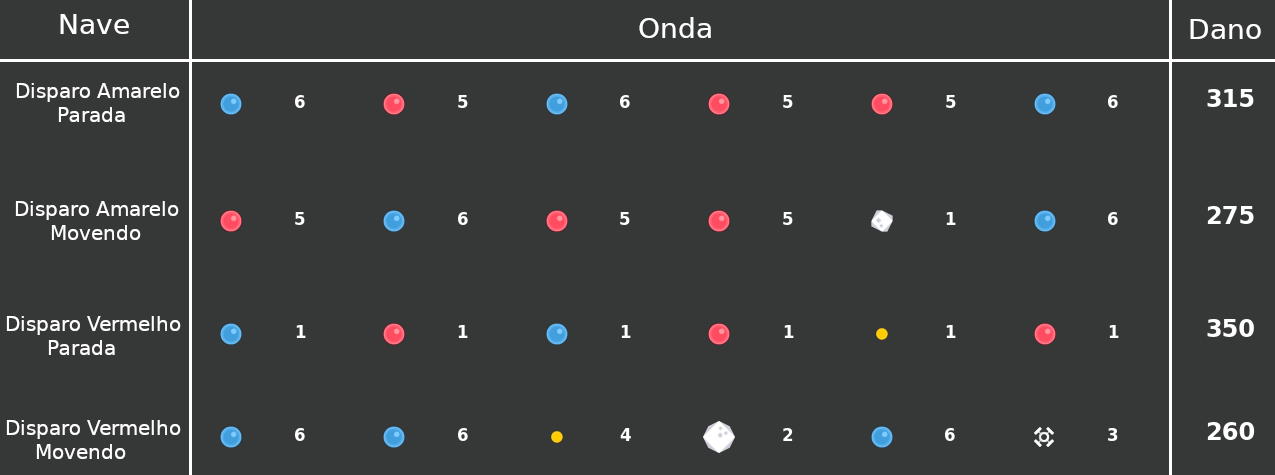
\includegraphics[width=1.0\textwidth]{ss/tab-ss-max.png}
  \caption{Visualização das ondas aleatórias com maior dano no Space Shooter.\label{fig:ss-rd-max}}
\end{figure}

\pagebreak

%% ------------------------------------------------------------------------- %%
\section{Fitness dos Jogos}
\label{sec:a-fitness}

\subsection{Fitness e Mutação}
\label{sec:a-fitness-mutacao-usados}

Foram testados três modelos de \textit{fitness} no algoritmo genético para o jogo \textit{Tower Defense}, buscando obter melhores resultados na geração de ondas; enquanto o jogo \textit{Space Shooter} foi testado somente com a primeira e a terceira versão. Foi adotada uma nomenclatura de versões para simplificar as referências no texto:

\begin{table}
\centering
\begin{tabular}{l|l|l}
                            & \textit{Fitness} (v1) & \textit{Fitness} (v2)  \\ \hline
Taxa de mutação (v1)             & TD e SS          & -                      \\
Taxa de mutação (v2)             &      -           & TD                     \\
Taxa de mutação (v3)             &      SS          & TD          

\end{tabular}
\caption{Relação dos fitness e taxa de mutação usados no TD e SS.}
\label{tab:fit-names}
\end{table}

%% ------------------------------------------------------------------------- %%
\subsection{Tower Defense - Fitness e Mutação}
\label{sec:td-fit}

O primeiro teste realizado utilizou uma função \textit{fitness} que considera se o alvo chegou ao final do trajeto e o quanto do trajeto foi percorrido, indivíduos que completaram o percurso serão muito mais recompensados e aqueles que morreram muito longe do alvo tendem a ser eliminados da população. A taxa de mutação decai conforme o tempo, começando em \textit {mutation\_prob} = 1.0 (100\%) e decrementando até 0. A taxa de mutação volta para 100\% a cada repetição do experimento (30 ondas). 

\begin{programruledcaption}{\textit{Fitness} do primeiro teste do \textit{TD} (v1).\label{prog:avaliacao_TD1}}
  \begin{lstlisting}[
    language={[brazilian]pseudocode},
    style=pseudocode,
    style=wider,
    functions={},
    specialidentifiers={},
  ]
        funcao fitness_v1 (x) // Dá uma pontuação para indivíduo \textbf{x}
            // reached\_goal(x) = booleana se chegou ou não ao final do trajeto
            se reached_goal(x)
                fit := 1
            senao
                fit := 0
            
            // offset(x) = quanto do percurso foi completado.
	        fit := (fit + offset(x)) / 2 // média aritmética dos valores de x
	        devolva fit // Um float com uma pontuação no intervalo [0,1].
        fim
  \end{lstlisting}
\end{programruledcaption}

\begin{programruledcaption}{Taxa de mutação do \textit{TD} para o primeiro teste (v1).\label{prog:mutacao_TD1}}
  \begin{lstlisting}[
    language={[brazilian]pseudocode},
    style=pseudocode,
    style=wider,
    functions={},
    specialidentifiers={},
  ]
        funcao mutation_v1 () 
            se mutation_prob >= 0
		        mutation_prob -= 0.05
		    ...
		    // continuação do processo de mutação.
        fim
  \end{lstlisting}
\end{programruledcaption}

Para o segundo teste, a função \textit{fitness} considera a quantidade do trajeto que foi percorrido (\textit{float} de 0 a 1) e a quantidade de vida ao final do trajeto (\textit{float} de 0 a 1), ou seja, inimigos que completarem o percurso serão mais recompensados conforme a quantidade de vida que chegaram ao final do trajeto. Note que indivíduos que morreram no caminho não serão bem recompensados com essa função. Por um erro, a taxa de mutação ficou em 1 a partir da segunda wave, contudo, alguns resultados interessantes foram obtidos também.

\begin{programruledcaption}{\textit{Fitness} do \textit{TD} (v2) (Avaliação, em português).\label{prog:avaliacao_TD2}}
  \begin{lstlisting}[
    language={[brazilian]pseudocode},
    style=pseudocode,
    style=wider,
    functions={},
    specialidentifiers={},
  ]
        funcao fitness_TD_v2 (x) // Dá uma pontuação para indivíduo \textbf{x}
            // offset(x) = quanto do trajeto foi percorrido, float de 0 a 1.
            // hp (x) = quanto de HP sobrou do inimigo, float de 0 a 1.
	        fit := (offset(x) + hp(x)) / 2 // média aritmética dos valores de x
	        devolva fit // Pontuação no intervalo [0,1].
        fim
  \end{lstlisting}
\end{programruledcaption}


\begin{programruledcaption}{Taxa de mutação do \textit{TD} para cada bateria de testes (2º par dos gráficos).\label{prog:mutacao_TD2}}
  \begin{lstlisting}[
    language={[brazilian]pseudocode},
    style=pseudocode,
    style=wider,
    functions={},
    specialidentifiers={},
  ]
        funcao mutation_v2 () 
            se geração = 1
		        mutation_prob := 1 / 12
		        
		    senão
		        mutation_prob := 1.0
		    ...
		    // continuação do processo de mutação.
        fim
  \end{lstlisting}
\end{programruledcaption}

Para o terceiro teste, a função \textit{fitness} considera a quantidade do trajeto que foi percorrido (float de 0 a 1) e a quantidade de vida ao final do trajeto (float de 0 a 1), idêntico ao anterior. Contudo, a taxa de mutação permanece em um valor fixo equivalente a $\frac{1}{12}$, conforme embasamento no estudo de \citet{haupt00:mutationprob}.

\begin{programruledcaption}{\textit{Fitness} do \textit{TD} (v3) (Avaliação, em português).\label{prog:avaliacao_TD3}}
  \begin{lstlisting}[
    language={[brazilian]pseudocode},
    style=pseudocode,
    style=wider,
    functions={},
    specialidentifiers={},
  ]
        funcao fitness_TD_v3 (x) // Dá uma pontuação para indivíduo \textbf{x}
            // offset (x) = quanto do trajeto foi percorrido, float de 0 a 1.
            // hp (x) = quanto de HP sobrou do inimigo, float de 0 a 1.
	        fit := ( offset (x) + hp (x)) / 2 // média aritmética dos valores de x
	        devolva fit // Pontuação no intervalo [0,1].
        fim
  \end{lstlisting}
\end{programruledcaption}

\begin{programruledcaption}{Taxa de mutação  v3 do \textit{TD} para cada bateria de testes (3º par dos gráficos).\label{prog:mutacao_TD3}}
  \begin{lstlisting}[
    language={[brazilian]pseudocode},
    style=pseudocode,
    style=wider,
    functions={},
    specialidentifiers={},
  ]
        funcao mutation_v3 () 
            mutation_prob := 1 / 12
		    ...
		    // continuação do processo de mutação.
        fim
  \end{lstlisting}
\end{programruledcaption}

%% ------------------------------------------------------------------------- %%
\subsection{Space Shooter - Fitness e Mutação}
\label{sec:ss-fit}

Conforme a Tabela \ref{tab:fit-names}, temos uma única função \textit{fitness} e as mesmas taxas de mutação 1 e 2 apresentadas na subseção anterior.

\begin{programruledcaption}{\textit{Fitness} de todos os testes do \textit{SS} (v1).\label{prog:avaliacao_SS1}}
  \begin{lstlisting}[
    language={[brazilian]pseudocode},
    style=pseudocode,
    style=wider,
    functions={},
    specialidentifiers={},
  ]
        funcao fitness_v1 (x) // Dá uma pontuação para indivíduo \textbf{x}
            // reached\_goal(x) = booleana se acertou o inimigo
            se reached_goal(x)
                fit := 5
            senao
                fit := 0
            
            // hp (x) = 5 * quanto de HP restou ao final da rodada.
	        fit := (fit + hp (x)) / 10 // média aritmética dos valores de x
	        devolva fit // Um float com uma pontuação no intervalo [0,1].
        fim
  \end{lstlisting}
\end{programruledcaption}%CONSERTADO, EU ACHO


%% ------------------------------------------------------------------------- %%
\section{Avaliação dos Testes de Versões de Algoritmo Genético}
\label{sec:fit-res}

 Para a avaliação dos algoritmos genéticos testados, foram gerados gráficos com a média de dano de cada i-ésimas ondas (de 1 até 30) e uma linha contínua com a regressão polinomial de grau 5 (\ref{prog:polyfit}), para os 30 experimentos em cada versão testada.
 
 Analisando os gráficos obteve-se a onda em que ocorreu a convergência do algoritmo, isto é, o ponto a partir do qual o dano causado pela onda ficou estável e aproximadamente linear.\footnote{Através de análise visual das linha de regressão polinomial, procurou-se o primeiro ponto de mínimo ou máximo - dependendo do comportamento crescente ou decrescente do algoritmo - a partir do qual a curva se mantinha razoavelmente estável. Testes que apresentaram resultados constantemente crescentes, decrescentes ou oscilantes foram considerados instáveis, onde o algoritmo nunca convergiu}

\begin{programruledcaption}{Trecho do código para cálculo da regressão polinomial.\label{prog:polyfit}}
  \begin{lstlisting}[
    language={Python},
  ]
    from numpy.polynomial import Polynomial
    
    fit = Polynomial.fit(df_1['wave number'], df_1['average damage'], deg=5)
  \end{lstlisting}
\end{programruledcaption}

A partir dos mesmos dados sem qualquer processamento - isto é, informações de 300 ondas com 6 ou 12 inimigos e o dano causado - foram gerados gráficos de \textit{boxplot}\footnote{Representação gráfica de localidade, viés e dispersão através dos quartis} padrão, com a média representada por quadrados vermelhos. Nestes é possível verificar a dispersão dos danos gerados pelo algoritmo, afim de verificar se o mesmo tende a chegar no mesmo resultado com consistência (indicados no gráfico por "caixas" mais compactas pois mais resultados de ondas se concentrariam de maneira próxima), ou se produz muitos resultados discrepantes, seja com dano muito alto ou muito baixo (graficamente seriam "caixas" longas, ou \textit{outliers}), e onde estão a a maior parte das soluções encontradas (onde a mediana divide os 30 experimentos pela metade e indica onde estão os resultados de dano mais frequente, enquanto a média pode ser influenciada por \textit{outliers}).

%% ------------------------------------------------------------------------- %%
\subsection{Tower Defense - Resultados}
\label{sec:td-fit-res}

Os gráficos seguintes (\ref{fig:fit-td-verde}, \ref{fig:fit-td-verm}, \ref{fig:fit-td-verd-verm} e \ref{fig:fit-td-verm-verd}) apresentam os resultados dos quatro casos de teste no jogo \textit{Tower Defense}, para as três opções citadas em \ref{sec:a-fitness-mutacao-usados}.

\begin{figure}[H]
  \centering
  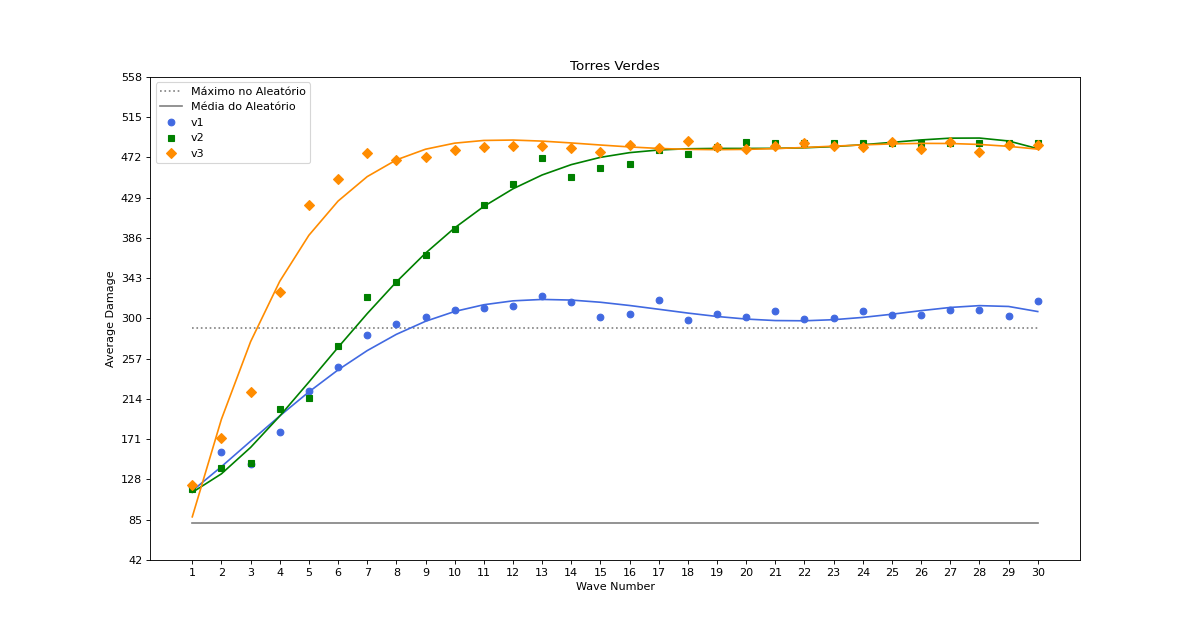
\includegraphics[width=1.1\textwidth]{td/Torres Verdes Fitness.png}
  \caption{Gráfico com as médias de dano para cada onda no teste com as Torres Verdes para as versões v1, v2 e v3.}
  \label{fig:fit-td-verde}
\end{figure}

\begin{figure}[H]
  \centering
  \includegraphics[width=1.1\textwidth]{td/Torres Vermelhas Fitness.png}
  \caption{Gráfico com as médias de dano para cada onda no teste com as Torres Vermelhas para as versões v1, v2 e v3.}
  \label{fig:fit-td-verm}
\end{figure}

\begin{figure}[H]
  \centering
  \includegraphics[width=1.1\textwidth]{td/Torres Verdes e Vermelhas Fitness.png}
  \caption{Gráfico com as médias de dano para cada onda no teste com as Torres Verdes + Vermelhas para as versões v1, v2 e v3.}
  \label{fig:fit-td-verd-verm}
\end{figure}

\begin{figure}[H]
  \centering
  \includegraphics[width=1.1\textwidth]{td/Torres Vermelhas e Verdes Fitness.png}
  \caption{Gráfico com as médias de dano para cada onda no teste com as Torres Vermelhas + Verdes para as versões v1, v2 e v3.}
  \label{fig:fit-td-verm-verd}
\end{figure}

As Figuras \ref{fig:td-box-green}, \ref{fig:td-box-red}, \ref{td-box-gr} e \ref{td-box-rg} a seguir mostram o comportamento, em cada teste, do dano total de cada i-ésima onda, cada uma sendo representada num \textit{boxplot}.

\vfill
\pagebreak

\begin{figure}[H]
  \centering
  \includegraphics[width=1.1\textwidth]{figuras/td/boxplot Torres Verdes.png}
  \caption{Boxplot do dano das 30 ondas nos 30 experimentos, para as versões v1, v2 e v3.}
  \label{fig:td-box-green}
\end{figure}

\begin{figure}[H]
  \centering
  \includegraphics[width=1.1\textwidth]{figuras/td/boxplot Torres Vermelhas.png}
  \caption{Boxplot do dano das 30 ondas nos 30 experimentos, para as versões v1, v2 e v3.}
  \label{fig:td-box-red}
\end{figure}

\begin{figure}[H]
  \centering
  \includegraphics[width=1.1\textwidth]{figuras/td/boxplot Torres Verde + Vermelha.png}
  \caption{Boxplot do dano das 30 ondas nos 30 experimentos, para as versões v1, v2 e v3.}
  \label{td-box-gr}
\end{figure}

\begin{figure}[H]
  \centering
  \includegraphics[width=1.1\textwidth]{figuras/td/boxplot Torres Vermelha + Verde.png}
  \caption{Boxplot do dano das 30 ondas nos 30 experimentos, para as versões v1, v2 e v3.}
  \label{td-box-rg}
\end{figure}

A Tabela \ref{tab:td-conver} mostra a onda aproximada onde o algoritmo parece ter convergido, e o dano médio após a estabilidade:

\begin{table}
\centering
\begin{tabular}{l|ll|ll|ll}
\multirow{2}{*}{Torres}                                     & \multicolumn{2}{l|}{v1} & \multicolumn{2}{l|}{v2} & \multicolumn{2}{l}{v3} \\
                                                            & Convergiu  & Dano Médio & Convergiu  & Dano Médio & Convergiu & Dano Médio \\ \hline
Verdes                                                      & 8          & 307.04     & 12         & 478.61     & 8         & 482.57     \\ \cline{1-7}
Vermelha                                                    & 15         & 157.78     & Não        & -          & 12        & 167.44     \\ \cline{1-7}
\begin{tabular}[c]{@{}l@{}}Verde +\\ Vermelha\end{tabular}  & 18         & 463.26     & Não        & -          & 11        & 288.18     \\ \cline{1-7}
\begin{tabular}[c]{@{}l@{}}Vermelha\\  + Verde\end{tabular} & 21         & 459.30     & Não        & -          & 12        & 399.16    
\end{tabular}
\caption{Tabela mostrando a onda onde ocorreu a convergência e o dano médio a partir desse ponto até o final.}
\label{tab:td-conver}
\end{table}

%% ------------------------------------------------------------------------- %%
\subsection{Tower Defense - Comparação}
\label{sec:td-fit-comp}

No \textit{Tower Defense} todas as versões do Algoritmos Genéticos se mostraram adequadas, superando a média da geração aleatória, entretanto no teste com Torres Vermelhas nenhuma superou o maior dano obtido em uma onda do teste \textit{Random}. Contra Torres Verdes existe uma solução ótima óbvia, tanques Verdes (\textit{EnemyGreen}), onde o inimigo com maior resistência (e portanto vida) é o mesmo com o maior dano, e as três versões testadas parecem chegar nesse resultado. 

Individualmente, as seguintes características foram apresentadas:

v1:
\begin{itemize}
  \item Convergência em todos os testes;
  \item Contra Torres Verdes apresenta a maior dispersão comparado com v2 e v3, mas o maior dano médio. Único caso onde a média e mediana ficaram próximas;
  \item Menor dispersão nos outros testes, após convergência;
  \item Exceto contra Torres Verdes, mostra dispersão inicial alta, quando converge concentra o dano no último quartil (Q4) e em \textit{outliers} próximos dos menores valores possíveis nas ondas repetidas, fornecidos na Tabela \ref{sec:uni-td}, mas com mediana acima da média;
  \item Não converge para um estado maximal contra Torres Vermelhas, mas consegue superar o maior dano aleatório (pois o melhor estado maximal detectado pela função \textit{fitness} é priorizar sobrevivência dos tanques ao invés do dano causado no Jogador);
  \item Maior dano, dentre as versões, contra Torres heterogêneas (Verde e Vermelha, Vermelha e Verde);
\end{itemize}

\pagebreak

v2:
\begin{itemize}
  \item Somente converge contra Torres Verdes - onde apresenta o segundo melhor resultado - concentrando resultados na mediana e em \textit{outliers} ligeiramente abaixo;
  \item Nos outros casos estabiliza de maneira oscilante, sem melhorar significativamente em relação a onda inicial, com poucos  \textit{outliers} mas muita dispersão (devido à taxa de mutação ser 100\% após a primeira onda);
  \item Consistente, com médias e medianas próximas.
\end{itemize}

v3:
\begin{itemize}
  \item Convergência em todos os testes, e mais rápida do que v1;
  \item Melhor resultado médio contra Torres Verdes - acima do maior dano aleatório - com dados concentrados no segundo e terceiro quartil, mediana acima da média e alguns \textit{outliers} ligeiramente abaixo;
  \item No teste contra Torres Vermelhas apresenta concentração de resultados entre a mediana no último quartil (Q4) e \textit{outliers} próximos das médias das piores ondas aleatórias;
  \item Apresenta a maior dispersão das versões do algoritmo contra Torres Verde + Vermelha, os quartis se estendendo desde o melhor resultado do v1 até os piores apresentados pelas ondas repetidas (Tabela \ref{sec:uni-td});
  \item Contra Torres Vermelha + Verde também supera o maior dano aleatório, com resultados concentrados entre a medianas no último quartil (Q4) e média, que foi afetada por \textit{outliers}.
\end{itemize}

Os resultados indicam que a versão v1 é bastante consistente, com baixa dispersão em 3 testes, mas corre risco de convergir em resultados longe do ótimo, possivelmente por progressivamente reduzir os genes aos piores candidatos e estabilizar no menos pior (taxa de mutação zera após a 20ª onda).

A última versão testada (v3) mostrou comportamento semelhante ao v1 mas com danos menores, exceto contra Torres Verdes. No restante não foi capaz de eliminar casos extremos onde estabilizou próximo do pior caso, apesar da pequena melhoria contra Torres Verde + Vermelha, provavelmente por reduzir os candidatos aptos por más escolhas, semelhante a v1.

\vfill
\pagebreak

%% ------------------------------------------------------------------------- %%
\subsection{Space Shooter - Resultados}
\label{sec:ss-fit-res}

Os gráficos seguintes (\ref{fig:fit-ss-ys}, \ref{fig:fit-ss-ym}, \ref{fig:fit-ss-rs} e \ref{fig:fit-ss-rm}) apresentam os resultados dos quatro casos de teste no jogo \textit{Space Shooter}, para as três opções citadas em \ref{sec:a-fitness-mutacao-usados}.

\begin{figure}[H]
  \centering
  \includegraphics[width=1.1\textwidth]{ss/Nave Parada com Disparo Amarelo Fitness.png}
  \caption{Gráfico com as médias de dano para cada onda no teste com a Nave Parada, Disparo Amarelo para as versões v1 e v3.}
  \label{fig:fit-ss-ys}
\end{figure}

\begin{figure}[H]
  \centering
  \includegraphics[width=1.1\textwidth]{ss/Nave Movendo com Disparo Amarelo Fitness.png}
  \caption{Gráfico com as médias de dano para cada onda no teste com a Nave Movendo, Disparo Amarelo para as versões v1 e v3.}
  \label{fig:fit-ss-ym}
\end{figure}

\begin{figure}[H]
  \centering
  \includegraphics[width=1.1\textwidth]{ss/Nave Parada Disparo Vermelho Fitness.png}
  \caption{Gráfico com as médias de dano para cada onda no teste com a Nave Parada, Disparo Vermelho para as versões v1 e v3.}
  \label{fig:fit-ss-rs}
\end{figure}

\begin{figure}[H]
  \centering
  \includegraphics[width=1.1\textwidth]{ss/Nave Movendo Disparo Vermelho Fitness.png}
  \caption{Gráfico com as médias de dano para cada onda no teste com a Nave Movendo, Disparo Vermelho para as versões v1 e v3.}
  \label{fig:fit-ss-rm}
\end{figure}




Semelhante a Seção \ref{sec:td-fit-res}, as Figuras \ref{fig:ss-box-green}, \ref{fig:ss-box-red}, \ref{ss-box-gr} e \ref{ss-box-rg} a seguir mostram o comportamento, em cada teste, do dano total de cada i-ésima onda, cada uma sendo representada num \textit{boxplot}.

\begin{figure}
  \centering
  \includegraphics[width=1.1\textwidth]{figuras/ss/boxplot Nave Parada com Disparo Amarelo.png}
  \caption{Boxplot do dano das 30 ondas nos 30 experimentos, para as versões v1 e v3.}
  \label{fig:ss-box-green}
\end{figure}

\begin{figure}
  \centering
  \includegraphics[width=1.1\textwidth]{figuras/ss/boxplot Nave Movendo com Disparo Amarelo.png}
  \caption{Boxplot do dano das 30 ondas nos 30 experimentos, para as versões v1 e v3.}
  \label{fig:ss-box-red}
\end{figure}

\begin{figure}
  \centering
  \includegraphics[width=1.1\textwidth]{figuras/ss/boxplot Nave Parada com Disparo Vermelho.png}
  \caption{Boxplot do dano das 30 ondas nos 30 experimentos, para as versões v1 e v3.}
  \label{ss-box-gr}
\end{figure}

\begin{figure}
  \centering
  \includegraphics[width=1.1\textwidth]{figuras/ss/boxplot Nave Movendo com Disparo Vermelho.png}
  \caption{Boxplot do dano das 30 ondas nos 30 experimentos, para as versões v1 e v3.}
  \label{ss-box-rg}
\end{figure}

A Tabela \ref{tab:ss-conv} mostra a onda aproximada onde o algoritmo parece ter convergido, e o dano médio após a estabilidade:

\begin{table}
\centering
\begin{tabular}{l|ll|ll}
\multirow{2}{*}{Nave}                                              & \multicolumn{2}{l|}{v1} & \multicolumn{2}{l}{v3} \\
                                                                   & Convergiu  & Dano Médio & Convergiu & Dano Médio \\ \hline
\begin{tabular}[c]{@{}l@{}}Disparo Amarelo\\ Parada\end{tabular}   & 18         & 163.54     & 13        & 147.66     \\
\begin{tabular}[c]{@{}l@{}}Disparo Amarelo\\ Movendo\end{tabular}  & Não        & -          & Não       & -          \\
\begin{tabular}[c]{@{}l@{}}Disparo Vermelho\\ Parada\end{tabular}  & Não        & -          & Não       & -          \\
\begin{tabular}[c]{@{}l@{}}Disparo Vermelho\\ Movendo\end{tabular} & Não        & -          & Não       & -         
\end{tabular}
\caption{Tabela mostrando a onda onde ocorreu a convergência e o dano médio a partir desse ponto até o final.}
\label{tab:ss-conv}
\end{table}


%% ------------------------------------------------------------------------- %%
\subsection{Space Shooter - Comparação}
\label{sec:ss-fit-comp}

No \textit{Space Shooter} nenhuma versão do algoritmo genético se mostrou adequada pois as ondas convergiram em um ponto não maximal de dano causado, e, em somente um caso, conseguiram dano maior do que na geração aleatória, nunca atingindo o dano máximo de uma dessas ondas. Individualmente, as seguintes características foram apresentadas:

v1
\begin{itemize}
  \item Consegue obter o mesmo dano da onda aleatória em dois testes - Nave Parada com Disparo Amarelo e com Disparo Vermelho;
  \item Com Disparo Amarelo apresenta alta dispersão e poucos \textit{outliers}, com média acima da mediana;
  \item Em particular, com a Nave Parada o algoritmo converge a um resultado não maximal, mas consegue gerar ondas de dano total próximo do máximo teórico (360) \ref{sec:uni-ss} (possivelmente, por priorizar os inimigos que sobrevivem mais ao invés de os que causam mais dano, uma vez que a função \textit{fitness} não prioriza o dano que cada tipo de inimigo causa);
  \item Em geral estabiliza de maneira oscilante, com ondas melhores e piores de maneira sequencial, e médias acima da mediana;
  \item Estabiliza com oscilação e taxa de dano decrescente no teste contra a Nave Parada e Disparo Vermelho, no entanto com diversas ondas que foram totalmente eliminadas, e algumas com dano próximo do máximo (um caso interessante, pois existem alguns tipos de inimigos que sobrevivem melhor em conjunto com outros tipos, mas morrem quando sozinhos e que se reproduz na natureza também, como a co-extinção);
\end{itemize}

\pagebreak

v3
\begin{itemize}
  \item No geral apresenta dispersão menos uniforme do que v1, com maior presença de \textit{outliers};
  \item Com disparo amarelo mantém média bastante acima da mediana, mas não chega a produzir ondas próximas ao máximo como v1, apesar de reduzir ocorrências de inimigos fracos;
  \item Converge no teste com Nave Parada e Disparo Amarelo;
  \item Apresenta o único dano acima da onda aleatória entre todos os testes contra a Nave Parada e Disparo Vermelho, onde possui pouca variação até a onda 10, quando começam \textit{outliers}, e a partir da 20 aumenta drasticamente a dispersão;
  \item Estabiliza de maneira oscilante, com taxa decrescente de dano nos testes com Nave Parada e Disparo Amarelo e Nave Movendo com Disparo Vermelho;
  \item Praticamente empata com o gerador aleatório no teste com a Nave Movendo e Disparo Vermelho, mas de maneira oscilante e viés decrescente, apresentando \textit{outliers} próximos do dano máximo possível.
\end{itemize}

Ambos os \textit{fitness} apresentam comportamento semelhante, onde as ondas iniciais melhoram os resultados coletivos - o dano total - mas progressivamente perdem eficiência, possivelmente devido a tentativa do algoritmo buscar os resultados melhores individuais mas sem a capacidade de detectar que a ordem de aparecimento potencializa o dano, pois a nave só pode atirar no asteroide que apareceu primeiro em seu raio de visão. Logo, é possível que um inimigo lento seguido de outros velozes maximizem o dano de uma rodada, ao "distrair" o jogador, mas que numa avaliação individual essa sequência de inimigos perca para outra onde um inimigo mais forte atingiu o jogador.

O Disparo Vermelho, que possui maior potência, pode ter produzido resultados fracos pois ondas que são totalmente eliminadas não oferecem oportunidade a detecção de candidatos para novas gerações, deixando o algoritmo sem opções de escolha.






\par

%% ------------------------------------------------------------------------- %%
\chapter{Considerações Finais}
\label{cap:consideracoes}

%% ------------------------------------------------------------------------- %%
\section{Análise dos Testes}
\label{sec:analise-testes}

Considerando os danos máximos teóricos e os danos médios dos casos repetidos, apresentados nas seções \ref{sec:uni-td} e \ref{sec:uni-ss}; os danos das ondas aleatórias mostrados em \ref{sec:rd-td} e \ref{sec:rd-ss}; e os testes do algoritmo genético em \ref{sec:td-fit-res} e \ref{sec:ss-fit-res}, utilizando os dados após a convergência dos algoritmos, obtemos as tabelas \ref{tab:td-allres-1} e \ref{tab:td-allres-2}, \ref{tab:ss-allres-1} e \ref{tab:ss-allres-2}:

\pagebreak

\begin{table}[H]
\centering
\begin{tabular}{l|l}
Torres Verdes                & Torres Vermelhas                    \\ \hline
Máximo Calculado = 540.00    & Máximo Calculado = 540.00           \\
\textbf{Fitness v3 = 482.57} & Repetido EnemyGreen = 360.00        \\
\textbf{Fitness v2 = 478.61} & Repetido EnemyBlue = 355.85         \\
Repetido EnemyGreen = 450.00 & Repetido EnemyRed = 180.00          \\
\textbf{Fitness v1 = 307.04} & Repetido OneEach = 167.82           \\
Repetido OneEach = 122.35    & \textbf{Fitness v3 = 167.44}        \\
Repetido EnemyPurple = 90.06 & \textbf{Fitness v1 = 157.78}        \\
Repetido EnemyRed = 89.90    & Repetido EnemyPurple = 127.60       \\
\textbf{Aleatória = 81.42}   & \textbf{Aleatória = 125.35}         \\
Repetido EnemyBlue = 60.68   & Repetido EnemyYellow = 50.58        \\
Repetido EnemyYellow = 40.07 & Repetido EnemyOrange = 50.00        \\
Repetido EnemyOrange = 39.93 & \textbf{Fitness v2 = Não Convergiu}
\end{tabular}
\caption{Dados agregados das médias de todos os testes, ordenado do maior para o menor no Tower Defense}
\label{tab:td-allres-1}
\end{table}

\begin{table}[H]
\centering
\begin{tabular}{l|l}
\begin{tabular}[c]{@{}l@{}}Torres Verde\\  + Vermelha\end{tabular} & \begin{tabular}[c]{@{}l@{}}Torres Vermelha\\   + Verde\end{tabular} \\ \hline
Máximo Calculado = 540.00                                          & Máximo Calculado = 540.00                                           \\
\textbf{Fitness v1 = 463.26}                                       & \textbf{Fitness v1 = 459.30}                                        \\
\textbf{Repetido EnemyGreen = 420.20}                              & Repetido EnemyGreen = 449.85                                        \\
\textbf{Fitness v3 = 288.18}                                       & \textbf{Fitness v3 = 399.16}                                        \\
\textbf{Repetido EnemyBlue = 220.18}                               & Repetido EnemyBlue = 329.82                                         \\
Repetido EnemyRed = 148.50                                         & \textbf{Repetido EnemyRed = 149.90}                                 \\
Repetido OneEach = 148.45                                          & \textbf{Repetido OneEach = 135.05}                                  \\
Repetido EnemyPurple = 120.00                                      & Repetido EnemyPurple = 120.00                                       \\
\textbf{Aleatória = 100.37}                                        & \textbf{Aleatória = 102.37}                                         \\
Repetido EnemyYellow = 50.00                                       & Repetido EnemyYellow = 50.00                                        \\
Repetido EnemyOrange = 44.50                                       & Repetido EnemyOrange = 49.45                                        \\
\textbf{Fitness v2 = Não Convergiu}                                & \textbf{Fitness v2 = Não Convergiu}                                
\end{tabular}
\caption{Dados agregados das médias de todos os testes, ordenado do maior para o menor no Tower Defense}
\label{tab:td-allres-2}
\end{table}

Em apenas 3 casos no jogo \textit{Tower Defense} o algoritmo genético foi capaz de atingir o maior dano, excluindo o dano teórico que só acontece quando o jogador não participa da partida - não faz nenhum tipo de \textit{input} exceto iniciar o jogo. Nos testes com as torres heterogêneas (Verde + Vermelha e Vermelha + Verde) o algoritmo genético com a versão v1 ultrapassou o dano de casos repetidos e para o caso com Torres Verdes a versão v3 consegue causar dano máximo. O projeto não teve como objetivo criar um oponente imbatível, para isso seria mais simples analisar como o jogador dispôs elementos de jogo e a partir disso desenvolver métodos pré-definidos de contra-ataque; ou até mesmo sempre utilizar ondas repetidas que maximizassem o dano, mas tais estratégias poderiam tornar o jogo frustrante ou repetitivo. Fazer com que a composição das ondas de inimigos de adéquem às condições de jogo é mais interessante, e o fato das ondas produzidas sempre superarem as ondas aleatórias neste caso mostram que uma potencial solução está sendo encontrada.

\begin{table}[H]
\centering
\begin{tabular}{l|l}
\begin{tabular}[c]{@{}l@{}}Nave Parada\\ Disparo Amarelo\end{tabular} & \begin{tabular}[c]{@{}l@{}}Nave Movendo\\ Disparo Amarelo\end{tabular} \\ \hline
Máximo Calculado = 360.00                                             & Máximo Calculado = 360.00                                              \\
Inimigo3 = 314.93                                                     & Inimigo3 = 213.20                                                      \\
Inimigo2 = 299.78                                                     & Inimigo2 = 184.61                                                      \\
OneEach = 82.75                                                       & Inimigo1 = 130.10                                                      \\
Inimigo1 = 181.50                                                     & \textbf{Aleatório = 124.95}                                            \\
\textbf{Aleatório = 181.26}                                           & OneEach = 100.85                                                       \\
\textbf{Fitness v1 = 163.54}                                          & Inimigo4 = 80.69                                                       \\
\textbf{Fitness v2 = 147.66}                                          & Inimigos = 67.79                                                       \\
Inimigo4 = 120.00                                                     & Inimigo5 = 39.23                                                       \\
Inimigos = 120.00                                                     & \textbf{Fitness v1 = Não convergiu}                                    \\
Inimigo5 = 60.00                                                      & \textbf{Fitness v2 = Não convergiu}                                   
\end{tabular}
\caption{Dados agregados das médias de todos os testes, ordenado do maior para o menor no Space Shooter}
\label{tab:ss-allres-1}
\end{table}

\begin{table}[H]
\centering
\begin{tabular}{l|l}
\begin{tabular}[c]{@{}l@{}}Nave Parada\\ Disparo Vermelho\end{tabular} & \begin{tabular}[c]{@{}l@{}}Nave Movendo\\ Disparo Vermelho\end{tabular} \\ \hline
Máximo Calculado = 360.00                                              & Máximo Calculado = 360.00                                               \\
\textbf{Inimigo3 = 241.60}                                             & Inimigo3 = 169.87                                                       \\
\textbf{Inimigo2 = 240.94}                                             & Inimigo2 = 169.67                                                       \\
OneEach = 125.99                                                       & OneEach = 96.99                                                         \\
\textbf{Aleatório = 123.66}                                            & \textbf{Aleatório = 91.77}                                              \\
Inimigo4 = 106.00                                                      & \textbf{Inimigo4 = 76.29}                                               \\
Inimigos = 102.44                                                      & \textbf{Inimigos = 65.89}                                               \\
Inimigo5 = 62.57                                                       & Inimigo5 = 39.26                                                        \\
\textbf{Inimigo1 = 27.60}                                              & \textbf{Inimigo1 = 24.60}                                               \\
\textbf{Fitness v1 = Não convergiu}                                    & \textbf{Fitness v1 = Não convergiu}                                     \\
\textbf{Fitness v2 = Não convergiu}                                    & \textbf{Fitness v2 = Não convergiu}                                     \\
Repetido EnemyOrange = 39.93                                           & \textbf{Fitness v2 = Não Convergiu}                                    
\end{tabular}
\caption{Dados agregados das médias de todos os testes, ordenado do maior para o menor no Space Shooter}
\label{tab:ss-allres-2}
\end{table}

Em contraponto, no jogo \textit{Space Shooter}, nenhuma versão consegue convergir em danos acima das ondas aleatórias, apesar de demonstrar potencial para isso contra a Nave Parada com Disparo Vermelho, mostrada no Gráfico \ref{fig:fit-ss-rs} - a taxa de dano é decrescente neste caso, então é possível que com mais ondas o algoritmo piore em relação ao aleatório. Em particular, nos testes com a Nave Parada e Disparo Amarelo (Gráfico \ref{fig:fit-ss-ys}) e Nave Parada com Disparo Vermelho (Gráfico \ref{fig:fit-ss-rs}) a versão v3 conseguiu aumentar o dano nas primeiras ondas, o que pode indicar compatibilidade em partidas curtas ou com redução mais agressiva na possibilidade de mutação, mas seriam necessários testes para confirmar tal possibilidade. No geral, é possível que a natureza menos determinística do estilo de jogo - onde é possível se movimentar para evadir inimigos, deixar de atacar algum oponente pra focar em outro, faça com que o algoritmo genético não seja tão eficiente quanto no \textit{Tower Defense}, que é um jogo mais estático e de comportamento bem definido - as torres não podem ser alteradas durante a onda, e todos os inimigos devem ser atacados para uma defesa efetiva. Seria possível alterar propriedades do \textit{Space Shooter} para diminuir a aleatoriedade da partido - por exemplo, pré-definir pontos de \textit{spawn} dos inimigos - mas acreditou-se que tais mudanças alterariam a natureza do jogo para forçar este se adequar ao projeto. Outro ponto levantado foi em relação à adequação da função \textit{fitness} que poderia levar em conta o dano causado pelos inimigos, já que a função prioriza muito a sobrevivência ao invés desse fator importante de métrica e os inimigos que mais sobrevivem eram justamente os que causavam menos dano.

%% ------------------------------------------------------------------------- %%
\section{Trabalhos Futuros}
\label{sec:futuro}

Considerando a efetividade do algoritmo genético no \textit{Tower Defense}, seria interessante estender os testes para geração de ondas com mudanças entre elas, pois num jogo normal o jogador iria adicionar ou aprimorar torres; o que implica que o algoritmo genético teria que potencialmente reiniciar o processo de convergência para uma geração ótima diferente do anterior. Também pode ser relevante considerar o dano coletivo ao invés de somente o individual dos inimigos, dando possibilidade do algoritmo detectar que está desviando de um estado maximal. Outro ponto que foi excluído por questões de tempo foram testes reais, com jogadores humanos, para obter \textit{feedback} sobre pontos como duração de jogo e escala de dificuldade - informações como essas permitiriam ajustes e testes posteriores em áreas como mutação e outros modelos de \textit{fitness} que seriam mais apropriados caso fossem necessários diferentes velocidade de convergência e escalada de dificuldade.

%% ------------------------------------------------------------------------- %%
\section{Conclusão}
\label{sec:conclusao}

Com os resultados obtidos, fica aparente que o algoritmo evolutivo implementado se mostrou mais adequado ao ambiente determinístico do jogo \textit{Tower Defense}, ao invés da aleatoriedade do \textit{Space Shooter}, causados pelas diferentes possibilidades de tiro (depende da primeira detecção do inimigo) e em dois testes da movimentação da nave. Seria possível tornar o \textit{Space Shooter} mais estático, com locais de \textit{spawn} mais distribuídos e pré-definidos, mas ao mesmo tempo o \textit{Tower Defense} deveria se tornar mais dinâmico, com as torres sendo atualizadas e adicionadas, alterando o ambiente onde o algoritmo genético está buscando evoluir. Dentro destes cenários, o projeto termina sem que seja possível verificar quais alterações seriam mais relevantes, tampouco as diversas adaptações que poderiam ser feita no código, buscando aceleração da convergência e evitando fuga de danos maximais. Ficou claro a infinidade de possibilidades a serem exploradas em um projeto com este tema.

De maneira mais pessoal, a primeira dificuldade da realização do trabalho foi a definição da proposta, posto que como grupo, cada um tinha diferentes ideias, porém eram vagas e carecendo de rigor e objetivo necessário. Para buscar desenvolver novas habilidades, além de exercer outras obtidas durante a graduação, o desenvolvimento de uma inteligência artificial para jogos, assim como o desenvolvimento dos jogos em si, pareceu ser uma proposta interessante. Inicialmente o projeto pareceu simples, mas com o decorrer do tempo o entendimento do problema não se mostrou trivial, e foi necessário algum tempo para compreensão da profundidade da proposta. Tempo excessivo foi gasto na obtenção de fontes e literatura sobre o tema, mas talvez parte dele pudesse ter sido melhor aproveitado na implementação, que se alongou para familiarização de todos os membros com o \textit{Godot} e depois para o desenvolvimento dos jogos. Com os jogos prontos e o algoritmo prototipado, a definição dos testes e coleta de dados se mostrou relativamente demorada, mas foram um dos estágios mais interessantes do trabalho, pois a existência de métricas para qualificar o algoritmo se mostrou muito útil e interessante. Apesar do desejo de aprimorar mais o algoritmo e os jogos, não há tempo hábil para o mesmo, mas a experiência se mostrou edificante e enriquecedora, e demonstrou bem como desenvolver um experimento com algum rigor científico.

\par

